\documentclass[a4paper,12pt]{article}
\usepackage[slovene]{babel}
\usepackage[utf8]{inputenc}
\usepackage{multicol}
\usepackage{fullpage}
\usepackage{guitar}
\usepackage{titlesec}
\usepackage{graphicx}
\setcounter{secnumdepth}{-1} 
\usepackage[absolute]{textpos}
\titleformat{\chapter}{\large\bfseries}{\thesection}{1em}{}
\titleformat{\section}{\Large\bfseries}{\thesection}{1em}{}
\titleformat{\subsection}{\large\bfseries}{\thesection}{1em}{}

\begin{document}
\pagenumbering{Roman}
\begin{titlepage}
\begin{textblock*}{297mm}(-6mm,-0mm)
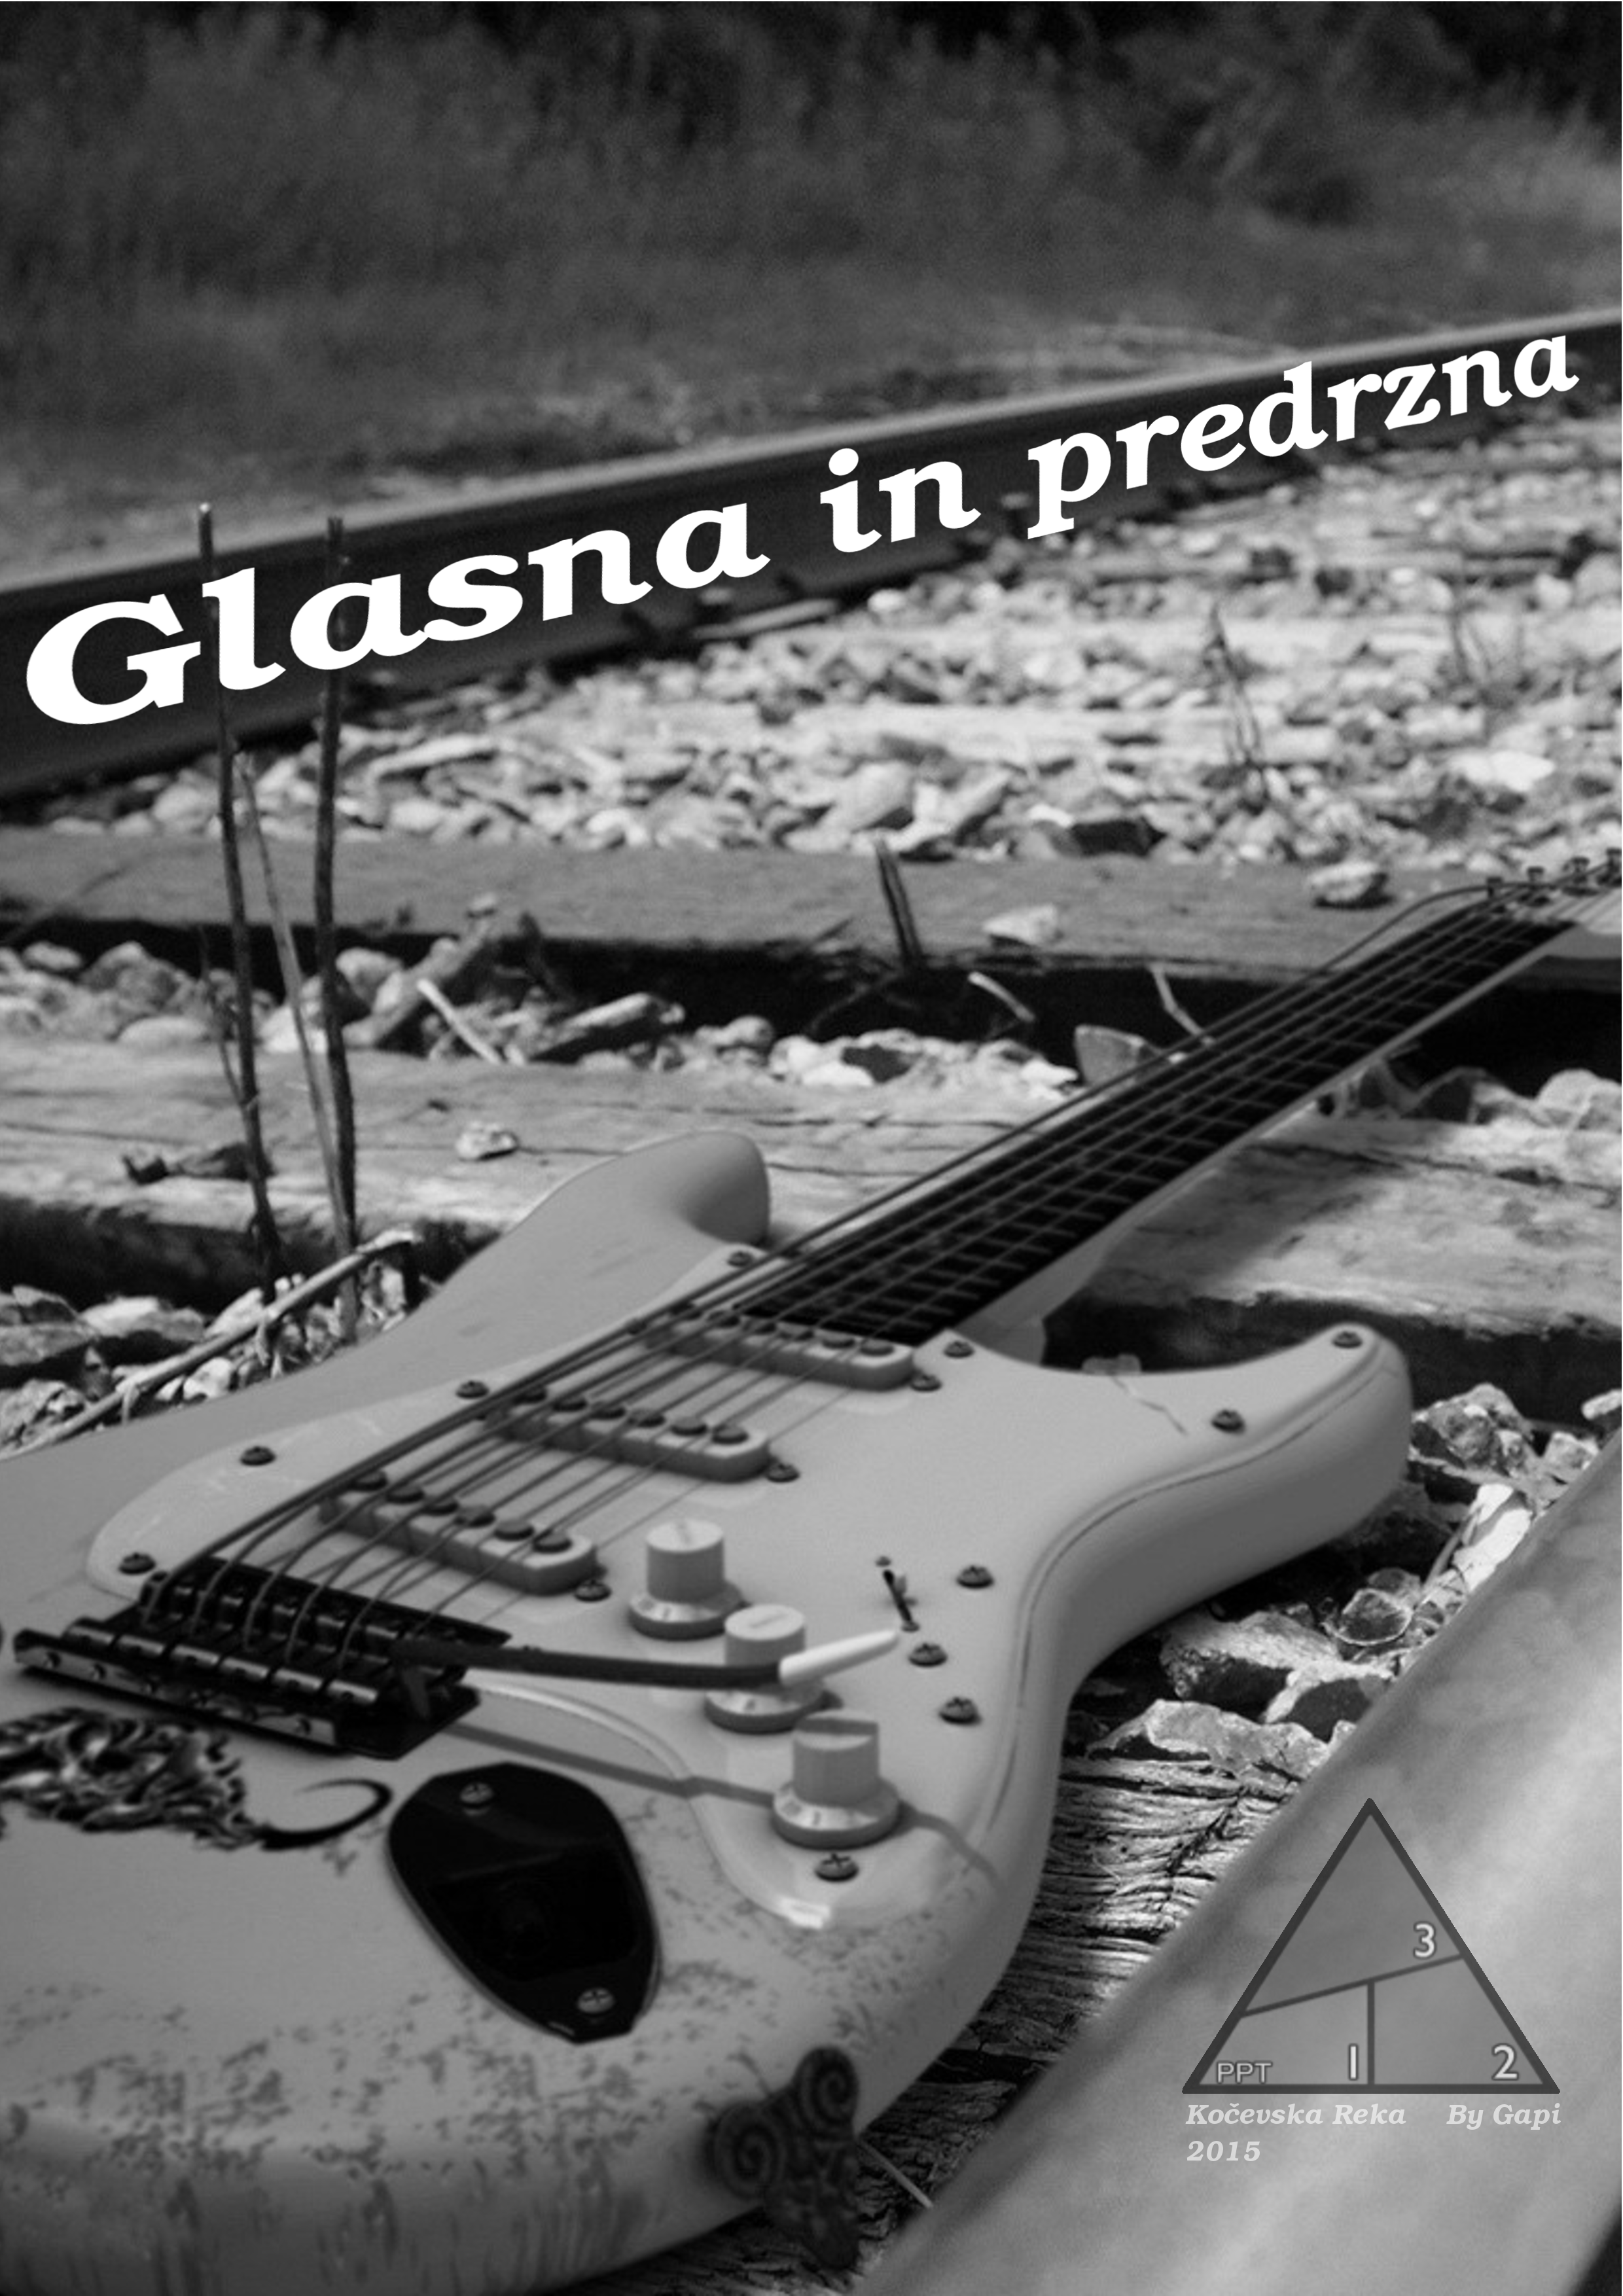
\includegraphics[width=\paperwidth]{img/tpage.png}
\end{textblock*} \
\end{titlepage}
\setlength{\columnseprule}{0.5pt}
\begin{multicols}{2}
\tableofcontents
\end{multicols}
\pagebreak

\setlength{\columnseprule}{0.5pt}
\begin{multicols}{2}
\pagenumbering{arabic}
\section{Akordi}
\begin{guitar}
[A - X02220  Am - X02210]

[B - X13331  Bm - X13321]

[C - X32010  Cm - X35543]  

[D - XX0232  Dm - XX0231] 

[E - 022100  Em - 022000] 

[F - 133211  Fm - 133111]

[G - 320003  Gm - 355333]

[H - X24442  Hm - X24432]


[A7 - X02020  B7 - X13131]

[C7 - X32310  D7 - XX0212]

[E7 - 020100  F7 - 131211]

[G7 - 320001  H7 - X21202]


[Am7 - X02010  Bm7 - X13121]

[Cm7 - X35343  Dm7 - XX0211]

[Em7 - 022030  Fm7 - 131111]

[Gm7 - 353333  Hm7 - X24232]


[C# - X46664  D# - 779997]

[F# - 244322  G# - 466544]


[C#m - X46654  D#m - 779987]

[F#m - 133111  G#m - 466444]


[A6 - X02222  C6 - X055555]

[D6 - X077777 E6 - X099999]


[ASUS2 - X02200]

[ASUS4 - X02230]

[DSUS2 - XX0320] 

[DSUS4 - XX0233]

[ESUS4 - 022200]

[CMAJ7 - X32000]

[FMAJ7 - 103210]

[GMAJ7 - 3X0032]

[DADD4/ADD2 - 554030]

\end{guitar}
\subsection*{Barre akordi}
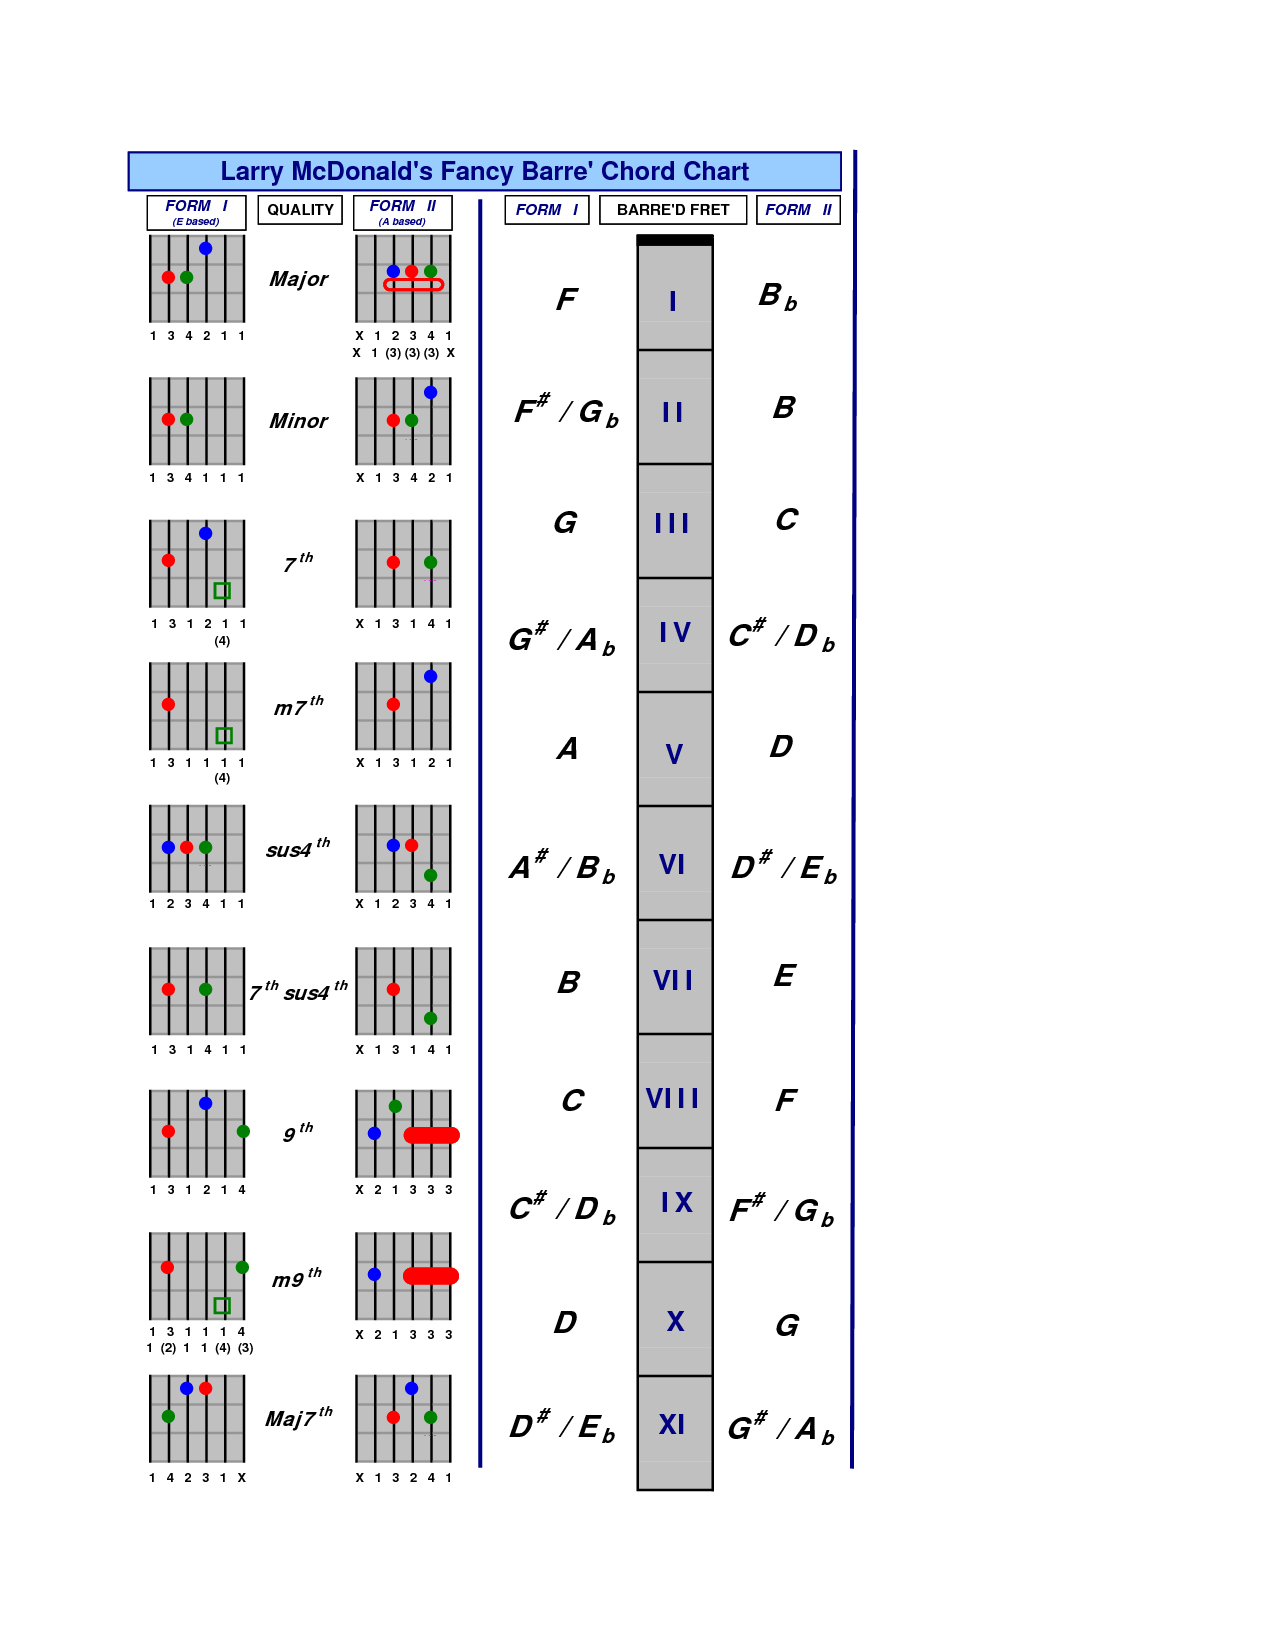
\includegraphics[width=140mm]{img/barre.png}
\clearpage
\section{2 dinara druže}
\subsection*{Riblja Čorba}
\begin{guitar}
[Am Am9 Am10/C Am9 Am]

[Am]Dečurliji [C]našoj smišljamo [Am]imena,
[Am]voleh je sve [C]više svaki božji [Am]dan,  
[C]ubedih se [G]najzad to je prava [Am]zena,      
[C]zajedno smo [G]stedeli za [F]stan.
Štedili za [Am]stan.


Sedeo sam tako sam za našim stolom,
sve što iole vredi, palo je u vodu,
opet me je žensko napravilo volom,
igrao samo epizodu.


[G]Htedoh da zaurlam strčao sam dole,
[Am]nisam mog'o [C]da izdrzim [Am]duže,
[G]socijalni slučaj pred vratima WC-a,
[F]rekao je: "Dva dinara druže! 
Dva dinara [Am]druže!"


[G]Mala nužda jedan, a velika dva.
[Am]pogledom ga sasekoh k'o [C]mačem,
[G]Izvinite molim, pitao sam ja,
[F]kol'ko košta kad unutra plačem? 
Kad unutra [Am]plačem?
\end{guitar}
\section{20 ljubic}
\subsection*{Adi Smolar}
\begin{guitar}
[Am]V ognju mam železja dost, 
ker nočem sam os[E]tat.
In zato kar 20 ljubic jest mam naen[Am]krat.
Vendar moti se, kdor misli, da lepo mi [Dm]je,
me vsaka le ob [Am]pamet spravlja [E]in mi živce [Am]zre.


Ena ljubica bi rada spremenila spol,
je druga splezala na poštarja in noče dol.
Tretja tolk je shujšala, da je nikjer več ni,
četrta je v arestu, peta pa v norišn'ci.


Hej! 
Jojmene, jojmene, jejhataja...


Šesta tolk zaudarja, da b' najraj jo pokopal,
sedma nora je ko noč, a hoče zmer' met prav.
Osma pravi: "Dnar mi daj, 
če hočeš z mano spat!",
deveta tolk teži, da bi najraj zavil ji vrat.


Hej! 
Jojmene, jojmene, jejhataja...


Moram vam priznat, deseta se kar gnusi mi,
"Najprej zdravje, pol kultura" pravi 
in ga kar spusti.
Sumim, da enajsta garje in uši ima,
na kup masti in žolce me spominja dvanajsta.


Hej! 
Jojmene, jojmene, jejhataja...


S trinajsto ah tko al' tko nikol ni sreče blo,
štirinajsto vse boli in zmer' ji je slabo.
Bi rada petnajsta postala nuna, 
nič nimam od nje,
šestnajsto pa nosi luna, hodi kdove kje.


Hej! 
Jojmene, jojmene, jejataja...


Sedemnajsto bi najraje v dom za starce dal,
osemnajsta tepe me odkar sem jo spoznal.
Za devetnajsto smisel žiljenja je prepir,
dvajseta nenehno vliva vase rum in pir.


Hej! 
Jojmene, jojmene, jejhataja...


V ognju mam železja dost, 
ker nočem sam ostat.
In zato kar 20 ljubic jest mam naenkrat.
Vendar fantiteta sinonim za srečo ni,
pameten le eno kvalitetno si dobi.
Pameten le eno kvalitetno si dobi.
\end{guitar}
\section{442 do Beograda}
\subsection*{Bajaga}
\begin{guitar}
[F A# 	F  Gm Gm F 2x]

[F]Ja imam krvotok od bencina,
pred mojim [A#]očima ravan [F]put,
ovo je žestoka ma[Gm]sina,
nebo mastilo, mesec [F]zut.

Nisam blesav, da brojim zvezde,
brojim znake i linije,
psi laju na karavane,
a karavane prolaze.

Kao tanak snar šušti prašina,
442 do Beograda,
gume škripe blues kilometara,
442 do Beograda.

solo

mozak radi na kiseonik,
ljubav okreče točkove,
motor svetli ko svetionik,
brzina skida okove.

Nisam blesav...

Kao tanak snar...

solo

Ja imam krvotok od...

Nisam blesav...

Kao tanak snar... 
\end{guitar}
\section{Adijo knapi}
\subsection*{Orleki}
\begin{guitar}
[F Am B F]

[F]Samo nekaj let je [Am]se ostalo,
in [B]gverk se bo za[F]prl,
za njim ostal bo spome[Am]nik na trgu
in ob [B]njem zarustan [F]hunt,
donferca ne [Am]bo vozila,
[B]kolma na šta[F]cjon,
ampak bo utruje[Am]na krasila
[B]nov ajzen[F]pon.


[Dm]Dvesto let je [Am]rod za rodom [B]grizel v to zem[F]ljo,
[Dm]Dvesto let je [Am]rod za rodom 
[B]preklinjal pod [F]zemljo.


Pesem krampov bo zamrla
in kamerati se bojo razšli,
nekam v kot v muzej se bo zadigal
v štil popljuvan herc.
Kdo odslej bo štrajke delal
in kdo frdinste klel
kdo odslej bo fano nosil
ko kak hajer bo umrl.


Dvesto let je rod za rodom grizel v to zemljo,
dvesto let je rod za rodom 
preklinjal pod zemljo.


Dvesto let...


Skozi vašhav bo le vahtar hodil,
skoz gezenke bo vleku prepih,
nihče ne bo več huntov rajdal
in nihče po hofu klel,
pesem krampov bo zamrla
in kamerati se bojo razšli
in ko se zadnji zajbrovc bo na britof znajdu
z njim umrl bo še spomin.


Dvesto let..
\end{guitar}
\section{Alojz valček}
\subsection*{Marko Brecelj}
\begin{guitar}
[C]Alojz Kod[Am]re mojster za [C]vse
Mojster za [G7]mafijo [C]mafijo
Alojz [Am]Kodre kriv si za [C]vse
Venem brez [G7]radosti [C]radosti
Toèka in [Am]pol človek in [C]pol
Človek brez [G7]milosti [C]milosti



Fleten kvar[E]tir preste in [Am]pir
Pesem in [E]smeh sanje [Am]so le
Mlade [E]oči dolge n[Am]oči
Kratek po[E]ljub kratka mla[Am]do[G]st



Šel bom na pot daleč od tod
Daleč od mafije mafije
Alojz brez vas v prostor in čas
V leta brez žalosti žalosti
Štempelj in pol služba in pol
Osem ur brez skrbi brez skrbi



Zrase mi sin zrase mi hčer
Leta prevesijo se v večer
Takrat za hip za bežen utrip
Vrne mi čas to pesem za vas



Alojz Kodre mojster za vse .....

\end{guitar}
\section{Balada}
\subsection*{Tantadruj}
\begin{guitar}
Ko pade [C]mrak, 
in siva [F]zvezda [G]se [C]utrne, [F G]'
[C]takrat odidem k l[F]ajdri vaso[G]vat. 

 
Ko sine z[C]ora, 
v meni s[F]e žel[G]odec [C]obrne. [F G]'
[C]Pijan sem bil in [F]nor, da [G]bi me [C]vrag! 


[G]Ne nisem [Am]Dante, ne Petrarka, 
tiho t[Em]one moja barka. 
še lju[F]bezen zvezd sem [C]pahnil na šta[G]cjon. 


Je reku [Am]Mičo, moj prjatu, 
ki se [Em]je s hudičem zbratu, 
da v ne[F]besih Bog ne [C]ve, kaj je par[G]don. 


Le pridi smrt, 
ki s svojo koso rada opletaš. 
Le brž, ker vlak za Had ne gre vsak dan! 


A bolje to, 
da si od mene nič ne obetaš. 
Pijan sem bil in od oblakov zapeljan. 


Ne nisem Dante...


Nazadnje še 
poduk za vas preroki s ceste. 
Za vas ki bojda kozmos vam je znan. 


Življenje šteje 
le za pir in slane preste. 
Kdor modruje je ob čas in ob denar. 

Ne nisem Dante...

\end{guitar}
\section{Balon}
\subsection*{Nude}
\begin{guitar}
[A]Ti si tok popularna,
[E]tvoje roke so zlatarna.
[A]In ko hodiš po mestu,
[D]vsak se za tabo ozre.  2X


[A]Lačna si ljubezni,
[E]jaz bom tvoj ulov.
[A]Dovolj si že stara,
[D]da se z mano igraš.

                   
In jaz te dam na ba[A]lon.
Pa tud če tvoja mama [Cis]me sovraži,
ker noče, da še kdo se s [D]tabo važi,
če boš [Hm]ti hotela kar ta[E]koj.


In jaz te dam na ba[A]lon.
Če slučajn bo te[Cis]zil tvoj stari,
dej povej mu, nej mi [D]ne sitnari,
ker to [Hm]stvar obvladam, se že [E]leta ubadam.


Jaz te dam na ba[A]lon.


Ti si tok popularna.
Vožnja je z balonom varna.
Če še vedno bojiš se,
glej jst mam velik balon.


Pokaž mi svojo sobo,
ker nočem več domov,
maš super rolete,
izklop si telefon.


In jaz te dam na balon...

\end{guitar}
\section{Beli prah}
\subsection*{Niet}
\begin{guitar}
[G C G C]

[Em]Preplašene [C]ptice brezglavo [D]so 
zbežale v ne[G]bo.
[Em]Se bolj brez[C]glavo 
[D]si begala [G]ti.


Toda nisi imela kril
in nisi vedela kam,
in sonce je umrlo
v tvojih očeh.


[G]Lep nasmeh včasih mi še poda[C]riš
za [D]beli prah,
[G]beli prah zdaj poljublja ti te[C]lo
[D]nič več jaz.


Lep nasmeh...


[G C G C]

V praznem pogledu tvojih oči, 
mrtvih oči,
iščem čas ki je minil.


Ko poslušaš šumenje dežja
in smeh noči
se spomni na naju nekoč.


Lep nasmeh... (2x)


V praznem pogledu tvojih oči,
mrtvih oči,
se spomni naju nekoč.

\end{guitar}
\section{Bolje biti pijan nego star}
\subsection*{Plavi orkestar}
\begin{guitar}
[Am]Kad po[E]mislim [Am]nate
stara ljuba[C]vi
[Dm]Zao mi je što smo [Am]bili
[C]samo dobri [E]drugo[Am]vi.


Al vrijeme leti, leti
mladost krača je
sve če jednom da se vrati
samo ona ostaje.


[Am]Bolje biti [E]pijan nego [Am]star
[Am]bolje biti [G]pijan nego [Am]star
[Dm]vino ne zna [Am]da smo nekad 
[E]bili sretan [Am]par
[Am]bolje biti [E]pijan nego [Am]star.


A kad dodje zima i prve pahulje
cekacu te moja buco kraj 1. gimnazije
neces,neces doci ja to dobro znam
mozda je i tako bolje
naviko sam biti sam.

\end{guitar}
\section{Bor do bora}
\subsection*{Taborniška}
\begin{guitar}
[C]Bor do bora, jelka z [G]jelko,
kakor gora, kakor [C]jeklo.
[C]Rod do roda, vsi v dru[F]zini,
smo v svo[C]bodni [G]dom[C]ovini.


[F]Sile močne, [C]sile, sile čvrste,   
[G]strnjene so v [C]naše vrste.
[F]Sile močne, [C]sile, sile čvrste
[G]naše vrste [C]so.


Šotor dom, narava mati,
oče grom, gozdovi brati.
Od sestra planin na morje,
širi, širi se obzorje.

          
Sile močne....


Glas severa, juga pesem 
tisočera v svet ponese
taborno nam geslo pravo:
Hej taborniki v naravo!

         
Sile močne....

\end{guitar}
\section{Bratovščina Sinjega Galeba}
\subsection*{Taborniška}
\begin{guitar}
[C]Pesem v vodah izgu[G]bljeno
plima prinaša na d[C]an.
[C]Trka na srca, da [F]gremo
pos[Dm]lušat jo noč in [G]dan.


[F]Morje se zgodaj pre[C]buja,
[F]preden rodi se [C]svit,
[Dm]ribice zlate ponuja,
[G]pojdi jih srečnež lovit.

 
[C]Mi vstajamo, jadramo,
kakor galebi na [G]pot.    
[G]V dalji ostajajo
pusti otoki [C]zmot.    
   

Mos[C]tove postavljamo,
družno od brega na [F]breg.
V pesmi, ki vsi jo [Am]sanjamo
[G]plove naš sinji ga[C]leb.

\end{guitar}
\section{Breakfast at Tiffany's}
\subsection*{Deep blue something}
\begin{guitar}
[D G A]  


You [D]say that [G]we've got [A]nothing in [D]common 
No [G]common [A]ground to [D]start from 
And [G]we're fal[A]ling a[D]part [G A]


You'll [D]say the [G]world has [A]come be[D]tween us 
Our [G]lives have [A]come be[D]tween us 
But [G]I know [A]you just don't [D]care [G A]


And [D]I said what about [A]breakfast at [G]Tiffany's? 
She [D]said, I think I re[A]member the [G]film,                 
And as [D]I recall, I think, 
we [A]both kinda [G]liked it.  
And [D]I said, Well, that's [A]one thing we've [G]got. 

 
I see you - the only one who knew me 
And now your eyes see through me 
I guess I was wrong 


So what now?  It's plain to see we're over, 
And I hate when things are over 
When so much is left undone 

\end{guitar}
\section{Budi moja voda}
\subsection*{Laufer}
\begin{guitar}
[C G F Em Am]


[C]Ostao sam [G]sasvim sam da [F]le[Em]zim na [Am]suncu
[C]Ja zvao sam te da [G]dodješ iz snova 
i [F]pru[Em]ziš mi [Am]ruku
[C]Ja molio sam da se [G]napune moja [F]mo[Em]ra i [Am]rijeke
[C]U njima još [G]jednom da osjetim 
novu [F]lju[Em]bav da [Am]teče


I pjevam...

[C]Budi moja vod[G]a, ja sam sada vatra
[F]iz[Em]gorjet [Am]cu
[C]Prolij se po me[G]ni, budi sve šta želim
[F]ja [Em]zivjet [Am]cu


Ostao sam sasvim sam da ležim na suncu
Ja zvao sam te da dodješ iz snova
i pružiš mi ruku
Ja znao sam da češ doći, doći i donijeti kišu
Ja čekao sam kao suha zemlja 
kad čeka svoju vodu


I pjevam...

Budi moja voda, ja sam sada vatra
izgorjet ču...


I kažem

Prolij se po meni, budi sve šta želim
ja živjet ču...

\end{guitar}
\section{Candy}
\subsection*{Iggy Pop}
\begin{guitar}
[G  C  Em]

It's a rainy afternoon 
In 1990
The big city geez it's been 20 years-
Candy-you were so fine


[G]Beautiful beautiful
[C]Girl from the n[Em]orth
[G]You burned my heart
With a [C]flickering [D]torch
I had a [Hm]dream that [C]no one else could see
You gave me [A7]love for [D]free [C D C]


[D]Candy Candy Candy
I can't [C]let you go [G] [A G]

All my life you're haunting me
I loved you so

Candy Candy Candy 
I can't let you go

[Em]Life is crazy [C]
[Em]Candy baby [C]


Yeah, well it hurt me real bad when you left
I'm glad you got out
But I miss you


I've had a hole in my heart
For so long
I've learned to fake it 
Just smile along
	    
    
Down on the street
Those men are all the same
I need a love
Not games, not games


Candy, Candy....

\end{guitar}
\section{Cotton fields}
\subsection*{CCR}
\begin{guitar}
[A]When I was a little itty bitty baby
my momma would [D]rock me in the [A]cradle
in them old cotton fields back [E]home
it was [A]down in louisi[A7]ana
just about a [D]mile from texar[A]kana
in them old [E]cotton fields back [A]home.

	
[A]When them [D]cotton balls get rotten
you can't [A]pick very much cotton
in them old cotton fields back [E]home
it was [A]down in louisi[A7]ana
just about a [D]mile from texar[A]kana
in them old [E]cotton fields back [A]home.


[A A D D A E7 A]

\end{guitar}
\section{Crazy game of poker}
\subsection*{OAR}
\begin{guitar}
Ohh myyyy

     
[C]20 throw [G]down in [Am9]my best [F]bridge
and the [C]man to my [G]left has folded [Am9]down [F]

well [C]Johnny doubled [G]up with a [Am9]royal fl[F]ush
I had [C]three jacks [G]and a pair of [Am9]nines [F]

my [C]mind is turning - [G]just two shots [Am9]more
there's [F]not much left to [C]play [G Am9 F]


Then dude walks in Black hat on top, 
what a mop
I'm lucky it wasn't a county cop
'Cause I'm just running out of time


Who's up for game two
what to do
my wallet's gettin thin
and I just lost my watch last night
well I gotta problem
just one answer
gotta throw it all down
and kiss it goodbye
Yeah!


That was a crazy game of poker
(That was a crazy game of poker)
I lost it all
(I lost it all)
but someday I'll be back again
And I, never to fall.
(never to fall)


Who's up for game three
I can barely see the bourbon 
drowning next to me
And I just lost it all
well there's a man sittin next to me
Red with smiling eyes
It's funny
I don't have no money tonight
yeaaaaaaaahhhhhhh


That was a crazy game of poker
(That was a crazy game of poker)
I lost it all
(I lost it all)
but someday I'll be back again
And I, never to fall.
(never to fall)


Bop bop bop...
I say now skittleedat dat,
Well how bout that?
I'm coming out the front 
never coming out the back


And I walked into the bar yesterday
Cause I had something to do, 
something to say
And Johnny walked in right behind me 
and I didn't turn around
Til I heard the sound of his feet 
falling on the ground
I looked over my shoulder and I saw a clown
And I said what'cha doin' in the bar tonight.


So I said Johnny whatcha doing tonight?
He looked at me with a face full of fright
And I said, how bout a revolution?
And he said right.
I say of, you say a
I say revolution, and you say jah
I say of, you say a
I say revolution, and you say jah jah jah
Jahova!


And I said, what'cha looking at?
He hit me across the face with a bat
I grabbed my .45 and I said let's get out and go
So he opened the door and said 
do what you're here for
I said I'm wandering round the road four to four
And I said 
I been walking for about a thousand years.


And my feet are growing tired
My eyes a little wired
Don't know what to do unless I retire
And he just said let's play some crazy poker


So I said Johnny whatcha doing tonight?
He looked at me with a face full of fright
And I said, how bout a revolution?
And he said right.
I say of, you say a
I say revolution, and you say die
I say of, you say a
I say revolution, and you say die dah dah
Day day oh!


I said that, was the craziest game of poker 
that I ever saw (2x)
But I'm not gonna quit and I'm not gonna stop
Don't give a shit cause I got the drop
Johnny just got two eyes just like mine
And I'm feeling kinda funky, kinda fine


And I drank a bottle of whiskey, 'fore I came
Came to the bar to see what's the same
I saw my man named Johnny 
sittin' across the table from me


And to my left was a man, he had no chin
Didn't really think about starting to sin
The man to my right wasn't feeling kinda nice
He looked kinda mad and I felt bad
Beacuse I took his money 
last night it's kinda funny
But now I'm just struggling--
I need a honey-bunny.
I don't know what to say anymore
So I'm just gonna go out, anywho...


So I said Johnny whatcha doing tonight?
He looked at me with a face full of fright
And I said, how bout a revolution?
And he said right.
I say of, you say a
I say revolution, and you say jah (3x)
I say of, you say a
I say revolution, and you say jah jah jah jahova
javhova, is watching over me...
Day day oh!  	

\end{guitar}
\section{Crazy little thing called love}
\subsection*{Queen}
\begin{guitar}
This [D]thing, called love, 
I [G]just [C]cant handle [G]it,
This [D]thing, called love, 
I [G]must [C]get round to [G]it,
[D]I aint ready, 
[Hb]Crazy little [C]thing called [D]love.


                   
This thing (This Thing) 
called love (Called Love)
It cries (Like a baby) In a cradle all night
It swings (Woo Woo) It jives (Woo Woo)
It shakes all over like a jelly fish,
I kinda like it
Crazy little thing called love 



There goes my [G]baby, 
she [C]knows how to rock and [G]roll.
She drives me [Hb]crazy, 
she gives me [E]hot and cold [A]fever,
then she [F]leaves me in a cool,cool sweat


[E E E E E E A]


I gotta be cool relax, get hip 
Get on my track's 
Take a back seat, hitch-hike 
And take a long ride on my motor bike 
Until I'm ready 
Crazy little thing called love 


I gotta be cool relax, get hip 
Get on my track's 
Take a back seat, hitch-hike 
And take a long ride on my motor bike 
Until I'm ready (Ready Freddie) 
Crazy little thing called love 


This thing called love I just can't handle it 
this thing called love I must get round to it 
I ain't ready 
Crazy little thing called love   8x

\end{guitar}
\section{Creep}
\subsection*{Radiohead}
\begin{guitar}
[G B C Cm]

When you were here be[G]fore
couldn't look you in the [B]eye
you're just like an [C]angel
your skin makes me [Cm]cry


You float like a feather
In a beautiful world
I wish I was special
You're so very special 


But I'm a creep
I'm a Weirdo
What the hell am I doing here?
I don't belong here


I don't care if it hurts
I want to have control
I want a perfect body
I want a perfect soul


I want you to notice 
when I'm not around
You're so very special
I wish I was special


But I'm a creep
I'm a weirdo
What the hell am I doing here?
I don't belong here.


She's running out again
She's running out
She runs runs runs runs runs


Whatever makes you happy
Whatever you want
You're so very special
i wish i was special


but i'm a creep
I'm a weirdo
What the hell am I doing here?
I don't belong here.

\end{guitar}
\section{Čakaj me}
\subsection*{Zoran Predin}
\begin{guitar}
[Hm  A  G]


[Hm]Mojih pet mi[A]nut je danes.
[F#7]Brez kravate in ve[Hm]zalk.
[Hm]In če mi še sto[A]pinje vzameš,
[F#7]bom kot plesalec brez ple[Hm]salk.



Mojih pet minut je danes.
Stražarji puškam pojejo.
Ko sonce jutru zarjo vname,
jim bodo pesmi vračale.


[Hm]Mislim samo [C]tiste misli,
[G]ki jih seveda ne bi [F#7]smel.
[Hm]In ko se vrnem, bom še [C]vedno tisti[G],
ki na postaji prosi [Hm] ča[A]kaj [G]me!


Danes se mi zdijo zvezde...
Na prste stopim in so tu.
Polne žepe jih prinesem!
Verjame sreča vitezu?


Mislim samo tiste misli...


[Hm]Potem bom samo tvoj heroj 
za večne skupne čase.
[A]Predpražnik, senca tvojega psa.
[G]Potem bom obešalnik, kahla za otroke,
[F#7]kava v postelji, ljubimec za oba.


Čakaj me...

\end{guitar}
\section{Čakal sem te kot kreten}
\subsection*{MI2}
\begin{guitar}
[C9 D C9 D]

[Am]Cakal sem te celo [C]jutro, 
celo [G]noč, večer in dan pred [G/Em]tem
[Am]od nikoder [C]ni bilo korakov, 
mobi[G]tel zaspal je gluh in [G/Em]nem
[Am]Je blo res vse tak na[C]robe, 
[G]da je treba blo kon[G/Em]cat
[Am]Kdo bo zdaj pre[C]našal moje fore,
 [G]kdo smejal se mi od [G/Em]vrat


[C9 D C9 D]


Zbrani v vrsti pod zastavo 
smo verjeli v neke boljše dni
gazili bi, jedli travo, 
brez besed prelili svojo mlado kri
za boga, za domovino, 
da bi zrušili oblast
za šteko čikov, liter vina, 
pa da malo vbijemo dolgčas


[D]Cakal sem te kot kre[C]ten
čakal neke [D]boljše čase
[H7]preveč butast, preveč [C9]len
[D]da bi mogo [G]mislit nase


Tam prek, čisto na začetku,
ko je svet še zadnjič bil iskren
V zavetju materninih prsi, 
dokler uka žeja bi me gnala ven.
Se podvizat da bi zrasel, 
se naučil, da bi razumel.
Da čimprej bi znal počet vse tisto,
kar kdo drug je mislo da bi htel.


Čakal sem te kot kreten... (2x)


In sem rilil kot kreten,
rinil v neke boljše čase, 
preveč butast, preveč len, 
da bi mogo mislt nase.


Vse življenje kot kreten,
sanjam neke boljše čase,
s tem da je ves vic v tem
kar daš podse, kar daš nase...

\end{guitar}
\section{Čez Šuštarski most}
\subsection*{Majda Sepe}
\begin{guitar}
[Dm G7 C Am Dm G C] 


[C]V Ljubljani, za Lj[E7]ubljanico,
tam [Am]najde vsak vse [C7]kar želi.
Tam [F]skrije med cve[C]tlice te [D7]Julija [G7]bar.
če s[C]i zaljubljen, [E7]ce si mlad.
[Am]a čez leto [C7]in čez dan
pri[F]sel boš tja z [C]nevesto, [G7]na Magi[C]strat.


[C]Cez [E7]Suštarski [Am]most[C7],
[F]Cez [C]Suštarski [D7]most.[G7]

[C]Levo na [E7]Mestni trg, [Am]desno na [C7]Stari trg.
[F]Po spomine [C]po mladost čez [G7]Suštarski [C]most.


V Ljubljani, za Ljubljanico, 
najde vsak kar išče.
Tam za večerjo Vitez kopuna ti da.
in Maček cvička rdečega
in če z mačkom greš  od tam,
lahko potunkaš  glavo v Robbov vodnjak.

Čez Šuštarski most...


[Dm]la la [G7]la  l[C]a la[Am] la[Dm]  [G]   [C]

[Dm]la la [G7]la  l[C]a la[Am] la[Dm]  [G]aa[C]aaa-ha 


V Ljubljani, za Ljubljanico, 
tam najde vsak kar išče-
fant sulico, mož cviček in luna balkon.
največjo knjigo učenjak, minikrilo deklica,
še tole svojo pesem, našla sem tam.


Čez Šuštarski most...


La la la la la la.........

\end{guitar}
\section{Da te vidim golu}
\subsection*{Babe}
\begin{guitar}
Ako me [G]voliš, dokaži to [C]i ne uzimaj za zlo
Što sam brz [G]bio, [F]kratko te [C]ljubi[G]o.
U tvome oku ne vidim sjaj, slutim i na skori kraj.
Baš mi se ne da, djavo me ujeda.

	     
[G]Da te vidim golu  ( daj da te vidim golu ) 
[C]na severnom polu ( na severnom polu ) 
[G]Da te vidim golu, [F]to sam po[C]zele[G]o.

Ti si za mene svetinja, ustvari si avetinja.
Ne budi takva veštica opaka.
U noči punog meseca, strah mi dušu preseča.
Srce mi kalnu na tebe brutalnu.

Da te vidim golu ( daj da te vidim golu ) 
na severnom polu ( na severnom polu )
Da te vidim golu, to sam poželeo.

\end{guitar}
\section{Dan ljubezni}
\subsection*{Pepel in kri}
\begin{guitar}
[A]Pusti tisoč dni in tisoč no[Hm]ci, ki jih več [D]ni,
če [E]sploh ne veš, da so kdaj bi[A]li. [E]


[A]Vzemi le en dan,
ki skril si ga [Hm]tja na srčno st[D]ran,
poz[E]abil ga ni[E7]koli več ne b[A]oš.[A7]


[D]To je bil tvoj dan ljubezni,
najlepši dan, ki ne [A]mine nik[A7]dar.
[D]Svet živi za dan ljubezni,
dan, ki da ti vse in vse ti v[A]zame,
tega nikdar ne v[E]eš.


[D]Kdaj [E]pri[A]sel bo zate [D]spet ta [E]dan,
[D]naj te [E]u-[D]pa-[A]nje ne zapusti.
[D]Le [E]za[A]spi, ko jutro [D]te zbu[E]di,
[D]to [E]bo ljubezni [A]dan.


To je bil tvoj dan ljubezni,...
Kdaj prišel bo zate spet ta dan,... 2x

\end{guitar}
\section{Danes bo srečen dan}
\subsection*{Tomaž Domicelj}
\begin{guitar}
[C]Vem da danes bo srečen dan, 
[G]to sem začutil že [C]zjutraj,              
[C]zagotovo danes bo srečen dan, 
[G]tudi to se zgo[C]di.


[G]Kaj če ladja bo re[C]sila brodolomca
in [F]dež bo padal kjer [C]suša že [F]traja vrsto [G]let.


Vem da danes bo srečen dan...


Morda se genij bo res nekje rodil 
in vojna se bo končala tam, kjer si vsi žele. 


Vem da danes bo srečen dan, 
to sem začutil že zjutraj,
upam pa da bo srečen dan, 
prav za vse ljudi. 2x

\end{guitar}
\section{Dekle moje pojdi z menoj}
\subsection*{Vlado Kreslin}
\begin{guitar}
[E]Dekle moje pojdi z me[D]noj,
[A]dekle moje pojdi z me[E]noj,
dol ob reki v tisti [D]beli obleki,
[A]dekle moje pojdi z me[E]noj.



A se zvezda tam na vodi blešči,
zvezda tam na vodi blešči,
ne to je venec, gizdavi na tvoji glavi,
to ni zvezda, ki se v vodi blešči.



Dekle moje pojdi z menoj,
dekle moje pojdi z menoj,
dol ob reki v tisti beli obleki,
dekle moje pojdi z menoj.



Je to mesec, ki tam z roso leži,
Mesec, ki z roso leži,
ne to sta najini postavi,
v mehki rosni travi,
to ni mesec, ki z roso leži.

\end{guitar}
\section{Dobra vila}
\subsection*{Tabu}
\begin{guitar}
[G]Včasih ko slo[H]nim ob oknu, [Em]gledam dol lj[C]udi.
[G]Zaskrbljene, [H]zamorjene, [Em]glave sklonje[C]ne.


Ona tiho solze skriva, on je ves na tleh.
Vse bi dala da zanetim iskrico v očeh.


A dala bi če bi postala, vila za en dan.
Njemu srečo, njej ljubezen, komu le nasmeh?


Tara ta ta......


Nihče več ne objokuje, nič več ni skrbi.
Nasmejano sonce sije na vse ljudi.


A naj udari, naj se sliši, glasno iz neba.
Naj prepeva naj odmeva pesem čudežna.


Tara ta ta... 2x


Skozi okno dobra vila gleda dol ljudi.
Pomagala Če bi znala najti ključ za vse skrbi.

\end{guitar}
\section{Dobro jutro}
\subsection*{Bajaga}
\begin{guitar}
[D]Dobro [G]jutro, [D]ovo iznad [A]nas je nebo
[D]Zna da [G]bude [D]kad je sunčan [A]dan
[D]Svetlo [G]plavo, [D]bistro dubo[A]ko i vedro
[D]Suncu [G]staza [D]a zvezdama [A]stan


Dobrodošli ova pesma to su ptice
Zatrepere kad je mesec pun
Lete nebom i pevaju kada sviče
Perje, krila, kap, duše i kljun


Dobrodošli pozdravlja vas divlje cveče
Sladak miris ima svaki cvet
Strast i ljubav, zuje pčele opijene
To je ono što pokreče svet

\end{guitar}
\section{Dobro jutro}
\subsection*{Riblja Čorba}
\begin{guitar}
[C]Svanulo je iznad [F]crkve [D7]svetog [G]Marka
[C]Cistaci u žutom [F]uli[D7]ce su [G]prali
[C]Kući su se vukli [F]paro[C7]vi iz [G]parka
[C]Sta smo mogli, mi smo [F]jedno [D7]drugom [G]dali


[G]Dobro [C]jutro. [F7 G C]


Otresaš sa suknje lisce i prašinu
Stružem s pantalona ostatke od blata
Polako i sigurno bežiš u tišinu
Čekaju te dole taksisti kod JAT-a


Dobro jutro.


[F]Cele noči [G]ti si forsirala [Am]konjak
[F]Jutro kvari [G]sinoč započete [Am]veze
[F]Zorom si me [G]sutnula ko poslednji [Am]dronjak
[F]Ja sam ti uz [G]piče dosao ko [Am]meze.


Dok veselo cvrkuču ptičice sa grana
Sakrivaš rukama razmazano lice
U ustima vučem trulez od duvana
U daljini laju đukci i lutalice


Dobro jutro.


Cele noči...

\end{guitar}
\section{Don't cry}
\subsection*{Guns N' Roses}
\begin{guitar}
[Am]Talk to me [Dm]softly
[G]There's something in your [C]eyes 
[Am]Don't hang your [Dm]head in sorrow
[G]And please don't [C]cry 
[Am]I know how you feel [Dm]inside, i've, 
[G]I've been there bef[C]ore
[Am]Somethin's [Dm]changin' inside you
[G]And don't you [C]know


[F]Don't you [G]cry [Am]tonight, I still love you baby.
[F]Don't you [G]cry [Am]tonight.                   
[F]Don't you [G]cry [C]tonight,                  
there's a heaven [Am]above you baby. 
[F]And don't you [G]cry [Am]tonight.

Give me a whisper. And give me a sigh. 
Give me a kiss before you tell me goodbye.
Don't you take it so hard now. 
And please don't take it so bad. 
I'll still be thinkin' of you.
And the times we had...baby.

Don't you cry tonight...

And please remember that I never lied. 
And please remember 
how I felt inside now honey. 
You gotta make it your own way. 
But you'll be alright now sugar. 
You'll feel better tomorrow. 
Come the morning light now baby.

\end{guitar}
\section{Đurđevdan}
\subsection*{Bijelo Dugme}
\begin{guitar}
[Am]Prole[G]ce na moje [C]rame sleće 
[Dm]Durđevak [Am]zeleni 
[Dm]Durđevak [Am]zeleni
[F]Svima [G]osim [Am]meni


Drumovi odoše, a ja ostah, 
nema zvijezde danice
Nema zvijezde danice, 
moje saputnice.


E i kome sada moja draga 
na đurđevak miriše
na đurđevak miriše, 
meni nikad više.


[C]Eee ee [Dm]eee 

[Am]Evo zore, [Dm]evo zore, [Am]bogu da se [Dm]pomolim 
[Am]Evo zore, [Dm]evo zore, [F]ej Đuđevdan je 
[Dm]A ja nisam [F]s onom [G]koju [Am]volim   


E i kome sada moja draga 
na djurdjevak miriše
na djurdjevak miriše, 
meni nikad više.


Njeno ime neka se spominje 
svakog drugog dana
Svakog drugog dana 
osim đurđevdana.

         
Eee-ee-eee...

\end{guitar}
\section{Ekološki manifest}
\subsection*{Slon in Sadež}
\begin{guitar}
[D G D G Em G A] 


[D]Kaj nam bo e[G]lektrika, 
[D]znanost, ari[G]tmetika, 
[Em]kaj nam bo vse s[G]vetsko znanje, 
[A]ce je od njega samo sranje. 


Zakaj kitare ružit na glas, 
gremo raje v tišino na vas. 
Ob tihem potoku meditirat 
je bolje kot se prepirat. 
   
   
Kaj nam bo tehnologija,      
če te od nje v črevesju zvija. 
Na svetu je vedno več bolezni, 
a ni bolš umret od ljubezni. 


[D]Dajmo vse ele[G]ktrarne izk[A]lopit 
[D]in vse to[G]varne poto[Em]pit. 
[A]V strugi reke, ki mogočna [D]tečee[Hm]ee, 
nov [G]svet poskusi[A]mo nar[D]dit. 


Da bo vsak otrok na tem svetu sit, 
dajmo še kapitaliste pobit. 
Zakaj bi morali vse plačevat?
A ni dovolj, da imaš prijatelja rad?  


Namest, da najstnik po netu srfa,     
bo srfal po valovih otoka Krfa. 
In vse bo prav in zrihtano tko, 
k da bi le pravljica bilo. 


Refren 2x

\end{guitar}
\section{Eks za eks ljubico}
\subsection*{Adi Smolar}
\begin{guitar}
[Hm]Danes nabral si bom že[D]lodec poln omame
[A]In čakal, čakal, [Em]da objame me!
[Hm]Odšla je ženska [D]in za njo zalujem!
[A]Namesto solza [Em]tolažbo potrebujem!


Potikam se iz oštarije v oštarijo,
jih tolk je, da od hoje noge me bolijo!
Pa kaj, če bom zapil kar celo plačo?
Kaj mi bo dnar? Jaz rabim dans pijačo!


[Hm]En liter, [D]dva litra, [A]trije litri, [Hm]pir in žganje.
Eks za ex ljubi[D]co! Za lju[A]bezen!
In za s[Hm]tare sanje!


In pijem, pijem, vse kar imajo,
zlijem vase, karkol mi dajo!
Pametn pravi: Hej pazi malo!
Srce pa: Pij ga, četud te bo pobralo!


En liter...


Ves svet vrti, vrti se kot za stavo,
srce nabija mi alkohol v glavo!
A čutim, da v meni raste sila!
Ne na žalost, ne boš me danes zvila!


En liter...


Popolni temi se približujem,
Le kje je ona, pijano se sprašujem.
Morda na Dunaju, morda v Parizu?
Oj delirij moj, vsaj ti si blizu!


En liter...


Ko sem pijan, ne žalujem! Ne!
Ko sem pijan žensk ne potrebujem! Ne, ne!
Utopim v želodcu svojo rano, 
mi je vseeno, vseeno kaj bo z mano!


En liter...

\end{guitar}
\section{Every rose has it's thorn}
\subsection*{Poison}
\begin{guitar}
We [G]both lie silently still, 
in the [C]dead of the night.
Although we [G]both lie close together, 
we feel [C]miles apart inside.
Was it [G]something I said, or [C]something I did,
did my [G]words not come out [C]right?
Though I [D]tried not to hurt you, 
though I [C]tried, 
but I guess that's why they say


[G]Every rose has its [C]thorn.
Just like [G]every night has its [C]dawn.
Just like [G]every [D]cowboy sings a [C]sad, sad song.
[G]Every rose has its [C]thorn.


Listen to our favorite song,
playing on the radio.
Well the DJ says loves a game of 
easy come and easy go.
But I wonder, does he know,
has he ever felt like this.
Well I know that you'd be here right now 
if I
coulda let you know somehow, I guess


Every rose...


[Em]Though it's been [D]a while now, 
I can [C]still feel so much [G]pain.
[Em]Like a knife that [D]cuts you
the wound [C]heals, 
but the scar, that scar [G]remains


I know I coulda saved our love 
that night if I'd known what to say.
Instead of making love 
we both made our separate ways.
And now I hear you've found somebody new, 
and that I never meant that much to you.


To [D]hear that tears me up inside 
and to [C]see you cuts me like a knife, I guess


Every rose...

\end{guitar}
\section{Fight for yourself}
\subsection*{Melissa Lara Clissold}
\begin{guitar}
[Am      G      Am]

[G]So I'm dictat[Am]ed by this drive, y[G]eah,
to play [Am]music every ni[G]ght.
I want to [Am]share the love in[G]side me,
my heart and [Am]soul they want to f[G]ight,
for what's right.


Ba-pa ta-ra-ta pa-ra-ra-ra-ra
pa-pa pa-ra-ra...


Now you can try and change the system,
from the inside or the out.
But remember what's important,
Is not to question your doubt,
about the change we need,
from the hands that bleed,
from the inactivity
and the hipocrisy that surrounds us.


The change we need,
from the hands that bleed,
from the inactivity
and the hipocrisy that surrounds us.


Now you may label me a hippie,
but I really don't give a damn.
It's easy to judge somebody,
when you don't know yourself deep down.


Ba-pa ta-ra-ta pa-ra-ra-ra-ra
pa-pa pa-ra-ra...


Now you can try and change the system...


Fight, fight, fight...!
Fight for yourself

\end{guitar}
\section{Frida}
\subsection*{Psihomodo pop}
\begin{guitar}
[C]Frida [E]je bila moja [F]kraljica
[C]Frida [G]je bila moja [Am]kraljica
[C]Frida [E]je bila moja [F]kraljica
ali [Am]nitko nije [F]bio [G]njezin [C]kralj [G]


Ja sam radio a ona je čekala 
Ona je čekala da padne mrak 
Ona se čudila sto ne znam uživati 
Ja sam joj rekao:'Hey honey nije to sam tak'
 

Pod nama su pucali kreveti 
Mi smo se pucali dok ne pukne dan 
Ja sam je gađao al nisam pogodio 
Taji metak nije dovoljan

 
Frida ja ti nisam dida 
Imas dobre uši slusaj kroz njih 
Ti si bila moja jedina pračka     
A ja sam bio samo sprih

\end{guitar}
\section{Gorska roža}
\subsection*{Andrej Šifrer}
\begin{guitar}
[D]Odšel bom tja kjer je daljši dan,
kjer se [G]mestni svet kon[D]ca.
[D]Kjer namesto asfaltnih cest
[A7]vodi le steza. [D]


Hiše razpršene so
kot jata plahih jerebic.
Čas utripa drugače če živiš
v eni od gorskih vasic.


Tisti večer sem žganje pil,
kot ga pije gospodar.
Bog mi v jezik je dal moči
in takrat sem jo spoznal.


Soseda mlada prisedla je
srečal njene sem oči.
Ko smo peli sem jo gledal,
kako se mi smeji. [D7]

  
[G]Gorska roža [D]caka me,
[A7]gorska roža, da [D]vrnem se,
[G]moji Špeli [D]iz planin,
[A7]pod srcem pustil [D]sem spomin.


Brez staršev je, a fantov ni,
ki bi ženili se v gore.
Zjutraj gre v tovarno
saj z majhno kmetijo pač ne gre.


Vzela me je čeprav sem bil
zanjo skoraj še otrok.
Naučila me je piti med,
a jaz sem dal ji svojih 18 let.


Gorska roža...


Od takrat sem pri njej živel,          
na gruntu ob koncu vasi.
Čez dan kitaro sem igral 
in ljubil Špelo vse noči.


Bil opran sem in vedno sit,
jedel kruh sem iz njene peči.
Vstajala je zgodaj, na delavski
avtobus se vedno mudi.


Gorska roža...


Ko zadnja košnja v kozolcu je,
čutiš hladen že objem.
Postajal sem nemiren, 
saj začutil sem jesen. 


Ki pravi:


O dreja poglej okrog,
zdaj postal si del planin.
O dreja jaz se bojim, 
da nekoč te ne izgubim.

\end{guitar}
\section{Greva pod objem gora}
\subsection*{Uroš Kuzman}
\begin{guitar}
[C]Ko lesk rosnih kapel zjutraj z [F]mestom [G]se zbu[C]di
[C]si zadnji zaspanci še [F]odgrinja[G]jo o[C]ci. 
[C]Kot cvet gorske rože vse [F]počasi [G]zacve[C]ti. 
[C]vsi obračajo glave, a mene [F]dolgo [G]ze več [C]ni. 


Ker to je [F]dan, [G]ko po[C]zabim na vse, 
to je da[F]n, [G]ko mi [C]moje srce 
bije l[F]e, [G]za ta [C]svet brez meja 
in tu za [F]hip dotakneš [G]se neb[C]a.


Oblaki sanjavi, svež je vonj cvetočih polj, 
kot pesem v glavi, meni nikdar ni dovolj. 
Kjer seže pogled mi se obzorje ne konča, 
neskončne so sanje, tu prostora je za dva. 


Ker to je dan... 


Daj, še [F]ti se pri[G]druži, stopi z [C]mano v korak, 
le src[F]e, smeh in [G]volja, [C]to zmore vsak,[Am] 

kje se [F]sanje prič[G]nejo, to [C]vema oba, 
pridi [F]greva pod o[G]bjem go[C]ra. 


Ker to je dan... 


Daj, še ti se pridruži... 

\end{guitar}
\section{Hajde, da ludujemo}
\subsection*{Tajči}
\begin{guitar}
[C]Ne moraš biti [F]bogat i lijep.
[C]samo budi dobar i po[G]kloni mi cvijet. 
[C]ne moraš biti [F]snažan i grub.
[G]da budeš za moj [C]svijet.

 
Ti si momak za pobijede 
dvije prave riječi biče dovoljne
plava zvijezda na nebu sja 
ti si onaj koji tajnu zna.


[G]Hajde da ludujemo [C]ove noči
[F]hajde za[G]ljubi se u [C]moje oči  
[F]tvoje su [G]usne kao [C]cokolada[F]

to mi se[G] dop[C]ada.

\end{guitar}
\section{Hej brigade}
\subsection*{Partizanska}
\begin{guitar}
[A]Hej brigade hitite, razpodite, zatrite
Poži[E]galce slo[E7]venskih do[A]mov.
Hej, ma[D]sinca zagodi, naj od[A]meva pov[E]sodi,
Naš poz[A]drav iz slovenskih goz[E]dov.
Hej, ma[D]sinca zagodi, naj od[A]meva pov[E]sodi,
Naš poz[A]drav iz slo[E]venskih goz[A]dov.

Kje so meje, pregrade, za slovenske brigade?
Ne, za nas ni pregrad in ne mej.
Po slemenih oblačnih in po grapah temačnih,
Vse od zmage do zmage naprej!

Čez poljane požgane tja do bele Ljubljane
Naša vojska prodre kot vihar.
Dokler tu so brigade, kdo nam zemljo ukrade,
Na slovenskem smo mi gospodar.

\end{guitar}
\section{Huda mravljica}
\subsection*{Romana Kranjčan}
\begin{guitar}

Bi[C]la je huda mravljica, 
[C]sest črnih nog je imela.
Je [F]migala, je [C]vohala, je [G]cisto pon[C]orela.


Bil[C]a je huda mravljica, po trgu je hodila,
lon[F]carju je čez [C]piskre šla,
pa [G]vse mu je po[C]bila.


In [F]kamorkoli je prišla,
so vsi pred njo be[C]zali,
je [F]pokalo, je stokalo, pod [G]njenimi stopali.


Oj, mravljica požrešnica, le kaj je naredila!
Še bika je pohrustala, samo roge pustila.
Seveda to je čisto res, le kaj se bik šopiri,
šest črnih nog 'ma mravljica, 
a bik ima le štiri.


Če slišiš hudo mravljico po svetu godrnjati,
obrni se in zbeži proč, kar zmorejo podplati.

\end{guitar}
\section{Hvala}
\subsection*{Rattlesnake}
\begin{guitar}
[Am Am7 F Am Am7 F#m]

[Am]Zadnji [E]zarek [Am]zaneti [E]prvo zvezdo,
[F]morje po[G]ljubi ne[C]bo[G].
[Am]klif strun[E]janski [Am]odene [E]se v temo,
[F]sliši se [G]pesem va[C]lov.


[C]Zvok kitare [F]in nes[G]končni ve[C]ceri,
vonj njenih [F]las mi [G]boža o[C]braz.
Vse kar kdaj sem [F]ljubil je [G]tik ob [C]meni,
ko jutranji [F]ogenj pre[G]lije se v [Am]dan.
     
            
Hladen veter zapiha na obalo,
meni je toplo.
Kot pomlad ki prežene zimo,
njeno mehko telo.

Zvok kitare...

Zvok kitare...

Vse kar kdaj sem ljubil je tik ob meni.
Vse kar sem želel je utrinek iz sanj.
Hvala ti za jutro po dolgi temi,
hvala za objem pod svodom neba.

\end{guitar}
\section{Hvala za vijolice}
\subsection*{Bilbi}
\begin{guitar}
[E]Ta tvoja žena mi je [Am]ze pri[E]jatelj' [Am]ca 
ne vem, če [E]ne bi ji kar [Am]vse po[E]veda[Am]la 
da skupaj [E]smirava od[Dm]kar tvoj [C]mali [G]Jan 
v [Dm]vrtcu [C]je vsak [G]dan. 


Ko prvič prišel si skoz’ vrata nasmejan, 
prevzel me je občutek – »vse lahko ti dam«, 
zdelo se mi je, da pač tak’ si strašno sam, 
da rabiš nežno dlan. 


[Am]Hvala  za  vijolice,
[Dm]torbe, čevlje, vrtnice,
[G]vse parfume, ogrlice.
Kaj pa [C]tvoje srce?
Kaj pa [E7]tvoje ime?  [Am Dm G C E7 ]


Hvala za počitnice 
in prekratke vikende, 
verze mal’ pocukrane. 
Kaj pa tvoje srce? 
Kaj pa tvoje ime? 


Postala sem čisto ta prava ljubica, 
kar dolgo časa nisem se zavedala, 
potem obljubljal si mi, da boš jo pustil, 
da boš se preselil. 


Ne upam ti pokazat, da mi je hudo, 
ker vse, kar primeš, ljubi, pade ti iz rok, 
ker zadnje čase nič več nisi nasmejan, 
z menoj si zadržan. 


Hvala za vijolice...

\end{guitar}
\section{I see fire}
\subsection*{Ed Sheeran}
\begin{guitar}
Oh, misty eye of the mountain below
Keep careful watch of my brothers' souls
And should the sky be filled 
with fire and smoke
Keep watching over Durin's [Em]son



If this is to [Em]end in [G]fire
Then we shall [D]all burn [C]together
Watch the [Em]flames climb [G]high [D]into the [Am7]night
Calling [Em]out fa[G]ther, [D]stand by and [C]we will
Watch the [Am7]flames burn 
[Hm]auburn on the [C]mountain side



And if we should die tonight
Then we should all die together
Raise a glass of wine for the last time
Calling out father, prepare as we will
Watch the flames burn 
auburn on the mountain side
Deso[Am7]lation [Hm]comes upon the [C]sky



Now I see [Em]fire[C],  [D]inside the [Em]mountain
I see [Em]fire[C],  [D]burning the [Em]trees 
And I see [Em]fire[C],  [D]hollowing [Em]souls
I see [Em]fire[C],  [D]blood in the [Am7]breeze
And I hope that you'll remember me



Oh, should my people fall
Then surely I'll do the same
Confined in mountain halls
We got too close to the flame  
Calling out father hold fast and we will
Watch the flames burn 
auburn on the mountain side
Desolation comes upon the sky


   
Now I see fire...



And if the [Em]night is [G]burning
I will [D]cover my [C]eyes
For if the [Em]dark re[G]turns then
My [D]brothers will [Am7]die
And as the [Em]sky's falling [G]down
It crashed [D]into this lonely [C]town
And with that [Am7]shadow upon the ground
I [Hm]hear my [C]people screaming [D]out

        

Now I see fire...



I see [Em]fire, 
oh you [C]know I saw a city [D]burning ([Em]fire)
I see [Em]fire, 
feel [C]the heat upon my [D]skin ([Em]fire)
And I see [Em]fire, 
[C]oooooo [D](fi[Em]re)
And I see [Em]fire burn 
[C]auburn on the [D]mountain [Em]side

\end{guitar}
\section{I shot the sheriff}
\subsection*{Bob Marley}
\begin{guitar}
[Em]I shot the sheriff
[Am]But I [Bm]didn't shoot 
no [Em]deputy, oh no! Oh!
[Em]I shot the sheriff
[Em]But I [Bm]didn't shoot 
no [Em]deputy, ooh, ooh, oo-ooh.


[C]All a[Bm]round in my [Em]home town,
They're [C]tryin' to [Bm]track me [Em]down;
They [C]say they want to [Bm]bring me in [Em]guilty
For the [C]killing of a [Bm]depu[Em]ty,
For the [C]life of a [Bm]dep[Em]uty.


But I say:
I shot the sheriff
But I swear it was in self-defence. 
I say: I shot the sheriff - Oh, Lord! -
And they say it is a capital offence. Yeah!


Sheriff John Brown always hated me,
For what, I don't know:
 Every time I plant a seed, 
He said kill it be-fore it grow
He said kill them be-fore it grow 


And so:
I shot the sheriff
But I swear it was in self-defence.
I shot the sheriff
But I swear it was in self-defence. 


Freedom came my way one day
And I started out of town, yeah!
All of a sudden I saw sheriff John Brown
Aiming to shoot me down,
So I shot - I shot - I shot him down and I say:


I shot the sheriff
But I didn't shoot no deputy, oh no! Oh!
I shot the sheriff
But I didn't shoot no deputy, ooh, ooh, oo-ooh.)


Reflexes had got the better of me
And what is to be must be:
Every day the bucket a-go a well,
One day the bottom a-go drop out,
One day the bottom a-go drop out.


I - I - I - I shot the sheriff.
Lord, I didn't shot the deputy. Yeah!
I - I (shot the sheriff)
But I didn't shoot no deputy, yeah! No, yeah!

\end{guitar}
\section{Imagine}
\subsection*{Beatles}
\begin{guitar}
[C]Imagine there's no [F]heaven.
[C]It's easy if you [F]try.
[C]No hell be[F]low us.
[C]Above us only [F]sky.
[F]Imagine [Am]all the peo[D7]ple [G]living for today.
[G7]A-ha-aaa


Imagine there's no countries
It isn't hard to do.
Nothnig to kill or die for 
And no religion too.
Imagine all the people living  life in peace 
Yu-hu-uuu


[F]You may [G]say  i'm a [C]dreamer. [E E7]

[F]But i'm [G]not the only [C]one. [E  E7]

[F]I hope some[G]day you'll [C]join us [E  E]

[F]And the [G]world will [C]be as one.


Imagine no posessions.
I wonder if you can.
No needs for greed or hunger 
A brother hood of man.
Imagine all the people sharing all the world.
Yu-hu-uuu.


You may say  i'm a dreamer.
But i'm not the only one.
I hope someday you'll join us 
And the world will live as one.

\end{guitar}
\section{Inštruktorska balada}
\subsection*{Beatles}
\begin{guitar}
[C]Vso noč ko tabor spi, [C7]sanjarim o njej,
ki rada ima lepe [F]reči.
[Dm]To se [G]zgodi [C]vsakemu, ki [C7]ljubi.
Lah[F]ko se zgo[G]di vsake[C]mu.
 

Ko noč zagrne travo, tišina zažari,
me misel nate greje, saj vem, da blizu si.
Topot zadrg šotorov me plaši,
da nisi potegnila tudi ti.

 
Ne vleci dol zadrge šotora svojega,
noč, ki je pred nama, bo sreča za oba.
Vodstvo sestankuje, ostali so odšli,
jaz pa sam prepevam, prepevam [C7]si.	
 

Inštr[F]uktorka [G]moja in [C]jaz inštruktor [C7]tvoj
in [F]Gozdna šola [Dm]z nama, 
[G]zdaj gremo vsi v [G7]boj - ooooj.
 

Spomin na tiste dni, na zvezdnate noči
prikliče melodijo mladostnih nežnosti.
Glej jo čarovnijo, spet veter šelesti.
Spet mi v mislih pesem oživi.


Ne vleci dol...

\end{guitar}
\section{Internat / Vsi ljudje hitijo}
\subsection*{Neca Falk}
\begin{guitar}
Skoraj [C]teden je že
odkar sem odšla iz
[F]naše vasi sem [C]dol.
[C]Sola začela se je zares,
[D]vstajam ob šestih in [G]pol.


Inter[C]nat je že star in
v sobi še s [F]tremi dekleti ži[C]vim,
Marta in Jana, obe sta iz morja,
a [G]Spela iz Gorenjskih pla[C]nin.


Mama tako je, kot rekla si mi,
da v začetku morda bo hudo,
saj prvič odšla si tak daleč od doma,
saj prej sploh ni časa bilo.


Pogrešam kmetijo, očeta in tebe
in malega Lukca vse bolj,
veš tu ni nič njiv in našega sonca,
tu je le sivi beton.


Na[F]mesto ptic zbudi me motor,
namesto [C]jutra srečam m[G]eglo
in [F]ves ta hrup, škripanje zavor,
kaj ti[D]sina je, tu sploh ne [G]vedo.


[C]Vsi ljudje hitijo, [F G]

[C]v panje, kjer živijo [F G]

z obrazi [C]obrnjenimi v [G]tla
nihče nikogar ne [C]pozna. [G]


Kako je doma, je Liska že strila,
nanjo mislim vsak dan,
v štali bo to zdaj prva sprememba
odkar bika prodali smo lan'.


In Florjanov Joža mi je dejal,
ko odhajala sem na to pot,
naj pošljem naslov mu,
češ da bo prišel v eni od prostih sobot.


Namesto ptic ...


Pozno je že, pismo končujem,
počasi odpravim se spat.
Že zdavnaj zaspal je s slikami doma
v solzah naš internat.

\end{guitar}
\section{JA!}
\subsection*{B. Terpinc, M. Koren, M. Stergar, D. Novak}
\begin{guitar}
[C]Kako je lepa, [G]kako diši
[Am]Zjutraj v glavi se [F]mi zvrti
[C]Iz šotorov slišim [G]godrnjanje,
[Am]vsi podaljšali bi [F]svoje sanje.


[C]Na Kolpi je ful [G]dobr – [Am]JA
[C]Ce nisi tle ni [G]dobr – [Am]ja
[C]Plaža in ma[G]saža – [Am]JA
[C]U kuhni pa sta[G]laža - [Am]ja


Globoko v senci kjer sonca ni
nova misel se rodi.
Ti ob meni, utrip srca,
prisluhni gozdu in šumu voda.


Ref.


Tam ob ognju njene oči.
V srcu čutim da si me želi.
Ne, ne, ne, ne, ne bom več oprezen.
V akcijo da rodi se ljubezen.


Ref.

\end{guitar}
\section{Jabolko}
\subsection*{Tantadruj}
\begin{guitar}
[G]Ne vem, za[C]kaj mi o[D]braz za[G]stiraš,
od daleč [C]jaz že te [D]prepo[G]znam.
Mojih p[C]oti tudi [D]več ne obira[G]s,
[C]zalostna si iz [D]dneva v [G]dan.


Kot jabolko, ki ga črv gloda,
ljubezen najina postala je.
Kot ena mlačna postana voda,
ki v sosednji luži je.


Da b' se takrat, ko bo red na sveti,
midva zopet srečala.
Če treba blo bi pa prej umreti,
vsak si druzga najdeva.

\end{guitar}
\section{Jagode in čokolada}
\subsection*{Rok'n' band}
\begin{guitar}
[C]Spominjam se [G]julijskih no[Am]ci,   [F]

[C]bili smo sami [G]morje, jaz in [Am]ti,   [F]

[C]bila si moja pesem, bi[G]la si moj edini [Am]zaklad, [F]

[G]nikoli nisem bil srečen kot sem bil ta[F]krat,
Neumen in ml[G]ad.


[C]jagode in [G]cokolada [Am]ne razmišljaj [G]ko si mlad[F]a,
[F]Srce naj te [C]vodi,
[Dm]in nič se ne [G]boj.


[C]jagode in [G]cokolada, [Am]naj spomine [G]ti pričara,
[F]Kadar boš z [C]drugim,
[Dm]ali z [G]menoj.


Spomnim se septembra prvega,
spet sva se v šoli srečala,
a hitro sem spoznal, da za vedno ti si odšla,
tam na šolskem vrtu
z drugim se poljubljala, ostal sem sam.


Jagode in čokolada…


[C]Jaz ljubim [E]jaz ljubim j[Am]o,
in naj vsaj [Dm]ona spi, č[G]e ne m[F]orem j[G]az


Jagode in čokolada…

\end{guitar}
\section{Jeans generacija}
\subsection*{Neki to vole vruće}
\begin{guitar}
[E]Kažu da je s one strane sad noć,
u toj zemlji, kažu, ponoć će proć'
i da je Johnny skinuo svoj stari [A]jeans.
A ovdje budi se [E]dan.


Oblačim na sebe isti taj jeans
i za Johnnya dižem ruku u vis,
spavaj Johnny, neka te ne plaši [A]mrak.
Mi isti dišemo [E]zrak.



[F#m]Nikada se [D]nismo susreli [F#m]mi,
kilometri [D]su nas dijeli[F#m]li.
Al' smo uvijek [D]isto mislili [E]mi, mi, mi!

Da, mi smo svi [A]jeans generaci[F#m]ja,
i mi smo sad [D]najjača naci[E]ja,
i mi smo i [A]istok i zapad i [F#m]jug,
mi smo to[D]variš, mister i [E]drug.


[E]Oblačim na sebe stari blue jeans
i za tebe dižem ruku u vis,
spavaj mirno, neka te ne plaši [A]mrak.
Mi isti dišemo [E]zrak.


\end{guitar}
\section{Jesen u meni}
\subsection*{Parni valjak}
\begin{guitar}
Ma što da [Am]zelim, sve je tako [E]daleko
I sad mi [Am]zao, sve bih opet [E]ponovo
[Dm]Najljepšu [G]pjesmu [C]tebi bih [E]pjevao
[Dm]Hej kamo [G]srece da sam [F]pjevat moga[E]o


Ptice u bijegu, tisina gradi zidove
Zvoni zbogom, rijeci kazne bozije
Te tvoje usne, opojne
Jos uvijek sanjam kako su me ljubile 


[Dm]Jesen u meni tuguje, zasto [G]sanjam [G7]cempre[C]se
Moje [Dm]ceste ne vo[E]de [Am]niku[A]da (bez tebe)
[Dm]Jesen u meni caruje, [G]a u [G7]tebi prolje[C]ce
Ni sunce [Dm]ne moze, [F]ne moze kroz obla[E]ke
Rano moja, [Am]hej ...


... s kime sada [E]putujes

Ma sto da bilo, nemoj da mi tugujes
Najljepsu pjesmu tebi bih pjevao
Hej kamo srece da sam pjevat mogao

\end{guitar}
\section{Jugoslavijo}
\subsection*{Narodna}
\begin{guitar}
[C]Od Vardara pa do Trigla[Dm]va,
[G]od Đerdapa [G7]pa do Jadra[C]na.
[C]Kao niska [D7]sjajnog đerda[G]na.
Svjetlim suncem [F]obasjana
[C]ponosito [D7]sred balka[G]na.
[C]Jugoslavijo, [G7]Jugoslavi[C]jo!



Širok svijeta put me vodio
za sudbom sam svojom hodio.
U srcu sam tebe nosio.
Uvijek si mi draga bila,
domovino moja mila.
Jugoslavijo, Jugoslavijo!



Volim tvoje rijeke i gore,
tvoje šume, polja i more.
Volim tvoje ljude ponosne.
I ratara i pastira
u frulicu kad zasvira.
Jugoslavijo, Jugoslavijo!



Krv se mnoga za te prolila,
borba te je naša rodila.
Radničaka te ruka vodila.
Živi sretna u slobodi,
ljubav naša nek' te vodi.
Jugoslavijo, Jugoslavijo!

\end{guitar}
\section{Jungle drum}
\subsection*{Emiliana Torrini}
\begin{guitar}
       
[Em]Hey, I'm in love,
My [G]fingers keep on [A]clicking to the 
[Em]beating of my heart.
[Em]Hey, I can't stop my feet,
Ebo[G]ny and [A]ivory and [Em]dancing in the street.

[Em]Hey, [F#]it's [G]because of you,
The world is in a [A]crazy, hazy [B]hue.


[C]My heart is beating like a [G]jungle [D]drum. (x2)
[C]My heart is beating like a [G]jun[F#]gle d[Em]rum.


Man, you got me burning,
I'm the moment between the 
striking and the fire.

Hey, read my lips,
Cause all they say is 
kiss, kiss, kiss, kiss, kiss.


No, it'll never stop,
My hands are in the air, yes I'm in love.


My heart is beating like a jungle drum. (x3)
My heart is beating like a jungle drum.


[D#]My heart is beating like a [A#]jungle [E#]drum. (x3)
[D#]My heart is beating like a [A#]jungle [G#]drum.


\end{guitar}
\section{Jutr}
\subsection*{Carpe diem}
\begin{guitar}
[H]Gledam TV, nikoli me ne mine,
[F#]ura je pol dve, v popku mam drobtine,
[E]cimer je lačen, teži kot zmeri,
[F#]ker ne najde pice od učeri.


[H]Vsak dan isto dolgočasim se doma,
[F#]na faks je beda, na pir se mi ne da,
[E]ničesar v življenju se več ne veselim,
[G]cas je da nekaj [F#]spremenim...


Za začetek se bom obriu in stuširu,
ne bom se več brezveze sekiral,
odnesu bom semti, šel v trgovino,
ker rabimo WC papir in čokolino.


Tamalo Tejo iz zgornjega štuka,
ki nabija po steni vedno ko ruka,
pelu bom na eno kavo,
začel bom laufat ker je zdravo!


Jutr jutr to bom naredu,
vjutr zjutri vse bo vredu,
vem da mi ne bo vseen,
ko zbudu se bom prerojen.


Jutr jutr to bom naredu,
jutr zjutri vse bo vredu,
spet si bom naredu plan,
vse skrbi bom vrgu stran.


Prjavu se bom na plesni tečaj,
vrnu knjige v knjižnico nazaj,
pospravu svinjarija za omaro,
dal bom nove strune na kitaro.


S frendi se ga šel bom nasekat,
s tastarimi se bom nehal prerekat,
ne bom več sedu cel dan doma,
in končno bom začel poslušat SKA.

\end{guitar}
\section{Kad sam bio mlad}
\subsection*{Riblja čorba}
\begin{guitar}
[Am]Sa trinaest sam popusio [G]prvu pljugu.
[Am]A posle prve [G]odmah i drugu.
Jer [G]tad... Tad sam bio [Am]mlad.



S četrne'st sam popio prvo pivo,
a posle piva sam pio sve živo,
Jer tad, tad sam bio mlad!



[G]Kad dobijem batine
[Am]nisam kukao
[G]bio sam tucen
[Am]i ja sam tukao
jer [G]tad...  Tad sam bio [Am]mlad.



Ja samo petnaest, ona ofucana
pala je ali bila je tucana
jer tad, tad sam bio mlad.



Sa sesnaest sam prvi put ponavljao,
pobeg'o od kuce i nisam se javljao
jer tad, tad sam bio mlad.



Malo sam lagao bio sam nagao.
Nikome racun nisam polagao.
Jer tad... Tad sam bio mlad.



\end{guitar}
\section{Kada padne noč}
\subsection*{Riblja čorba}
\begin{guitar}
[Am]ja zivim na slepom koloseku
prosli su svi moji vozovi
[F]cito sam danasnje novine
[Am]nisu izvuceni moji lozovi


sunce izlazi i zalazi
sve je kao i obicno
kada o tebi ne razmisljam
stvarno se osecam odlicno


[Dm]a kada padne [C]noc
ja [Gm]zovem u po[F]moc
jer [C]tebe nema [B]tu uuuu [Dm]'


[C]svaki novi dan
ko [Gm]smrt je dosa[F]dan
jer [C]tebe nema [B]tu uuuu [Dm]'


nisam dripac ni probisvet
i ni zbog ceg nije me stid
imam svoj mali svet
i oko njega kineski zid


sunce izlazi i zalazi
sve je kao i obicno
kada o tebi ne razmisljam
stvarno se osecam odlicno


a kada padne noc...

\end{guitar}
\section{Katjuša}
\subsection*{Partizanska}
\begin{guitar}
[Am]Zacvetele jablane in [E]hruške
[E]vstale so meglice iznad [Am]rek
[C]prišla [G]je na [F]strmi breg K[Am]atjuša,
[Dm]prišla [Am]na vi[E]soki strmi [Am]breg.


In zapela pesem čez poljano
o sokolu s širnih je planjav
in o njem, ki ljubi ga vdano,
ki ji pismo drobno je poslal!


Ti letiš od drugih ptic hitreje,
mojo pesem nesi v daljni kraj.
Partizanu, ki nam brani meje,
lep pozdrav Katjušin mu predaj!


Misli naj na ljubici edino,
ki mu pesem poje čez gore.
Naj ohrani našo domovino,
jaz ohranim svoje mu srce.

------------------------------------

Rastsvetali iabloni i grushi,
Poplyli tumany nad rekoj.
Vykhodila na bereg Katyusha,
Na vysokij bereg na krutoj.


Vykhodila, pesniu zavodila
Pro stepnogo, sizogo orla
Pro togo, kotorogo liubila,
Pro togo, chi pisma beregla.


Oj ty, pesnia, pesenka devichia,
Ty leti za iasnym solntsem vsled.
I bojtsu na dalnem pograniche
Ot Katyushi peredaj privet.


Pust on vspomnit devushku prostuiu,
Pust uslyshit, kak ona poet,
Pust on zemliu berezhet rodnuiu,
A liubov Katyusha sberezhet.

\end{guitar}
\section{Ker te nima rad}
\subsection*{Tomaž Domicelj}
\begin{guitar}
[D]Ko ponoči te drugi objema,
[A]zelim srečo obema,
[G]a kaj, ko te nima [D]rad.


Ko pomislim, da drugi te boža
poka mi koža,
saj te nima rad.


Če se spomnim, da drugi vate gre
trga se mi srce,
ker te nima rad.


[D]Je to moj poraz, ali [A]usoda?
Zakaj bi bi[G]la zvesta do [D]groba?
Te pesmi ne [G]pojem zato
da bi zopet privabil ti [D]solze v oči;
le zate me skr[A]bi, [G]ker te nima [D]rad.


Ne velja obljuba nobena,
si postala tistemu žena,
ki te nima, ki te nima rad.


Si gradove v oblakih gradila,
kar si imela si izgubila,
saj te nima, saj te nima rad.


Če imela z njim boš otroka,
te vseeno čaka moja roka,
ker te nima, ker te nima rad.


Je to moj poraz, ali usoda?
Zakaj bi bila zvesta do groba...

\end{guitar}
\section{Kiše jesenje}
\subsection*{Prljavo kazalište}
\begin{guitar}
[A]Nočas mladi mjesec [D]sja,
dobro veče dame [E]sve,
spustam se u baro[A]ve. 
 


Neki klinac,  
nasu pjesmu svira,  
i to me strasno zivcira, 



[E]Ej curo šećeru, 
[A]Nemam ja za veceru,
[E]Za malu votku raki[A]ju. 
[E]Hej curo šećeru, 
[A]ja sam ptica nebeska
[E]I to je moja sudbi[A]na.



[D]Kroz moje [E]prazne dže[A]pove 
vjetrovi mi [D]prolaze
A kroz c[E]ipel[A]e 
kiše j[D]esen[E]je

\end{guitar}
\section{Klub ljudi z resnimi težavami}
\subsection*{Zmelkoow}
\begin{guitar}
Če ti zj[C]utraj ko je kriza avto ne vžge 
[Am7]in ti med dopustom vedno ribica umre 
[Dm]stalno živiš v krizi identitete 
ne [G]znaš raztrgat perforirane serviete 


če ti obup redno skače pred oči
smrt te voha in po šunki ji dišiš 
v boljšo prihodnost ceste ni nobene 
rad bi bil zver a si le malo ščene 


[C]Pridi pogledat v nas novi klub
sami [Am7]težki pacijenti vrženi na kup 
[Dm]vsakega muči vsaj ena težava 
[G]vsak bo prisegu da njegova je prava 
[C]mali Karlo je že kot otrok 
[Am7]skužu kaj je to kvalitativni preskok 
[Dm]samo iz mase ljudi z velikimi problemi 
lahko [G]pridejo ven tako dobri refreni; [Am]


[Am]Problemi s[F]o problemi [G]bojo 
in kurc jih [C]gleda 
[Am]problemi s[F]o problemi [G]bojo 
in klinc jih [C]gleda seveda 
[Am]problemi s[F]o problemi [G]bojo 
in klinc jih [C]gleda 
[Am]problemi s[F]o problemi [G]bojo al pa [C]ne
vsako [F]tolko tudi [G]kakšen od njih umr[C]e 
vsako [F]tolko [G]


Če se ti dojenčki smejejo v obraz 
ko se smejiš ti vedno škripa glas 
ostaneš trezen še po dvajseti pivi 
gledaš v kamne in misliš da so živi 


Ob dobri priliki hitro zamižiš 
ko je šla mimo greš za njo in jo loviš 
čim mine panika postane dolgočasno 
kar imajo drugi je zmeraj najbolj krasno


Pridi pogledat...

\end{guitar}
\section{Ko so lipe cvetele}
\subsection*{Orlek}
\begin{guitar}
[G]      

Prijetno popoldne in [D]hladen vetric
pod [C]krošnjami [D]starih dre[G]ves
klopca v gaju, brs[D]tenje v maju
po[C]slušava [D]ptice žgo[G]let.


Najprej malo malce, sprošceni klepet
kako lepo je živet
gradiva nacrte tvoje oči so zazrte
v serijo mojih besed.


Pa sva [Em]sanjala vikend na [C]mor[D]ju
gra[Em]dila bajto v za[C]gor[D]ju
tako le[Em]po je sanjati v [C]dvo[D]je
da ni [D]res (da ni res) 
to ni [D]res (to ni res).
 

Ko so [G]lipe cvetele in [D]bil je lep maj
sva [C]sla na sprehod v [G]gaj 
ko so lipe cvetele [D]in je bil maj 
sem na [C]klopci obljubil ti [G]raj.


Mobi v tvoji torbi kar naprej je brencal
najraje bi ga v grmovje zagnal
postala si živcna kasneje še izbircna
pocasi izgubljam te.


Pa sva sanjala vikend na morju
gradila bajto v zagorju
nato pripeljal se on je z BMWjem
in si šla (in si šla) 
si odšla (si odšla).


Ko so lipe cvetele in bil je lep maj
sva šla na sprehod v gaj
ko so lipe cvetele in je bil maj
sem na klopci obljubil ti raj.


Ko so lipe cvetele...


Os[C]tal je spo[D]min na [G]maj
os[C]tal je sp[Hm]omin na [G]maj.

\end{guitar}
\section{Ko-Po}
\subsection*{Zmelkoow}
\begin{guitar}
[Em G C D Em]

Ko po[G]gledam to ne[C]bo 
[D]bi te najrajši ugriznu v koleno. 
[Em]In ko [G]voham to [C]travo 
[D]tam na vrtu nepokošeno.


Mi je [C]zal da nisem bol [Em]nor. 
Bi se [G]vlegel na njo in se [D]drl ko žival. 
Mi je [Em]zal da nisem bol v[C]trgan. 
Bi do [G]konca življenja dol na [D]hrbtu ležal.


Ko zagledam te oči 
me valovi potunkajo v sanje.
In pod vodo se mi zdi,
da je cel svet tu samo zame.


Bi ga ujel in gledal v luno 
in tulu v njo kot najbolj zmešani psi.
In potem bi hladno zaspal 
tako trdno kot lahko le truplo zaspi.

\end{guitar}
\section{Krokodilčki}
\subsection*{Čuki}
\begin{guitar}
[D]Modna pista [G]to je [A]prava [D]stvar, [G A]'
[D]lepe punce - [G]te so božji [A]dar, [G A]'
[D]glej jo, glej jo, [G]ta bo [A]miss sve[D]ta, [G A]'
še [D]spat ne morem, [A]ker želim si [D]da:


Njene dolge no[G]ge z mano v [A]stric bi h[D]odile,
le poglej njen nas[G]meh, kroko[A]dilčke v o[D]ceh.
Modna pista ods[G]lej bo po [A]mojih ko[D]lenih,
sam bom čuval nas[G]meh, kroko[A]dilčke v o[D]ceh,
[A]v o[D]ceh!


Sam se zdaj potikam naokrog.
Daleč stran od njenih dolgih nog.
Daleč stran od modnega sveta,
vendar si želim še vedno da:


Njene dolge noge...   

\end{guitar}
\section{Lahko bi zletela}
\subsection*{Vlado Kreslin}
\begin{guitar}
[prehod: C H G F#]

[Em]Hej, pa [C]to sem že [Am]videl,
[Em]To sem [C]ze doži[Am]vel, 
[Em]Stal pod [C]tvojim ok[Am]nom,
[Em]Ljubo[C]sumje [Am]grel.



Kdo je s kom in [Em]koga, [C Am] \
Kdo vse bil je z [Em]njo, [C Am] \
Sami znani ob [Em]razi, [C Am] \
Sami predol[Em]go. [D]



Lahko bi zle[G]tela
[C]In u[Am]jela [D]svoje [G]sanje, [C Am] \
Lah[D]ko bi se [G]dvigni[C]la
Na [Am]njih vse [D]do ne[G]ba. [C Am] \


Lah[D]ko bi zle[G]tela
[C]In u[Am]jela [D]svoje [G]sanje, [C Am] \
[D]Lahko bi se [G]dvigni[C]la
Na [Am]njih vse [D]do ne[G]ba. [C D] \



Vse te stare zamere
Merijo do srca,
Zatemnjeni pogledi
Nam ne dajo sna.
Kdo je s kom in koga,
Komu je mar za to,
Stokrat že premleto
življenje je kratko.
Lahko bi zletela
In ujela svoje sanje,
Lahko bi se dvignila
Na njih vse do neba.

\end{guitar}
\section{Latrina}
\subsection*{RSK}
\begin{guitar}
[C]V gozdu majhna jama,
nad jamo majhna bajta,
do bajte ozka stezica drži.
To [F]naša je latrina,
nam druga domovina,
ki vedno daleč naokrog smrdi.
Ooo-[G]ooo, kaj bi brez [C]nje.


[C]Ce preveč si se [G]napil in mačka i[C]maš.
Na latrino [G]stopiš in se poko[C]zlaš.
Če te trebuh bo[G]li, močno tiš[C]ci,
s palomo na se[G]kretu se vse ure[C]di.


Lalalalalala-laj....


Vsak dan ob vsaki uri
odpirajo se duri
in vrsta spet pomakne se naprej.
Preklinja in vzdihuje in nikdar ne miruje,
da luknja bi bila spet čimprej frej.
Ooo-ooo, kaj bi brez nje.


Če preveč si se napil...


Tam Romči galopira, 
si durco že odpira,
hiti, da bi oddal kar je odveč.
A glej ga šmenta, vraga,
tam drugi že odlaga
in kaže da ne misli nič več preč.
Ooo-ooo, ubogi Roman.


Saj tisti, ki je not sploh noče ven, 
saj se uresničil mu davni je sen.
Skoz špranje se reži, glasno prdi,
da z latrine daleč okrog vse smrdi.


Lalalalalala-laj...

\end{guitar}
\section{Leaving on a jetplane}
\subsection*{John Denver}
\begin{guitar}
[D7]

All my [G]bags are packed, I'm [C]ready to go,
I'm [G]standing here out[C]side the door
I [G]hate to wake you [C]up to say good[D7]bye.
But the [G]dawn is breakin', it's [C]early morn',
The [G]Taxi's waitin', he's [C]blowin' his horn.
Al[G]ready I'm so [C]lonesome I could [D7]die.


So [G]kiss me and [C]smile for me,
[G]Tell me that you'll [C]wait for me,
[G]Hold me like you [Am]never let me [D7]go.
'Cause I'm [G]leaving [C]on a jet plane,
[G]Don't know when [C]I'll be back again[G].
Oh [C]babe, I hate to [D]go.


There's so many times I've let you down, 
so many times I've played around.
I tell you now they don't mean a thing.
Every place I go I'll think of you, 
Every song I sing I sing for you.
When I come back I'll bring 
your wedding ring.


So kiss me ...


Now the time has come to leave you, 
one more time let me kiss you,
Then close your eyes, I'll be on my way.
Dream about the days to come,  
When I won't have to leave alone,
About the times I won't have to say.

\end{guitar}
\section{Lemon tree}
\subsection*{Fool's garden}
\begin{guitar}
[Em Hm Em Hm Am Hm Em]

[Em]I'm Sitting Here In A [Hm]Boring Room
[Em]It's Just Another Rainy Sunday [Hm]Afternoon
[Em]I'm Wasting My Time I Got [Hm]Nothing To Do
[Em]I'm Hanging Around I'm [Hm]Waiting For You
But [Am]Nothing Ever Happens [Hm]

And I [Em]Wonder


I'm Driving Around In My Car
I'm Driving Too Fast I'm Driving Too Far
I'd Like To Change My Point Of View
I Feel So Lonely I'm Waiting For You
But Nothing Ever Happens - And I Wonder


[G]I Wonder How I [D]Wonder Why
[Em]Yesterday You Told Me 'bout The [Hm]Blue Blue Sky
And [C]All That I Can [D]See 
Is Just A YeLlow [G]Lemon-tree [D]


I'm [G]Turning My Head [D]Up And Down
[Em]I'm Turning Turning Turning Turning
[Hm]Turning Around
And [C]All That I Can [A]See
Is Just A Yellow [D]Lemon-tree.


[Em Bm Em Bm Am Bm Em]


I'm Sitting Here I Miss The Power
I'd Like To Go Out Taking A Shower
But There's A Heavy Cloud Inside My Head
I Feel So Tired Put Myself Into Bed
Where Nothing Ever Happens - And I Wonder


[H]Isolation - [Em]Is Not Good For Me.
[D]Isolation - [G]I Don't Want To
[H]Sit On A Lemon-tree.


I'm Steppin' Around In A Desert Of Joy.
baby anyhow i'll get another toy.
And Everything Will Happen - And You'll Wonder


I Wonder How I Wonder Why...

\end{guitar}
\section{Lepa janja}
\subsection*{Bajaga}
\begin{guitar}
[D]Maslina je oliva [A]mene sunce poliva
[Hm]procvale su kajsije [F#m]rumene
[G]pa se vidi jasnije
[D]pa se čuje glasnije
[A]na celom svetu od sto milja.


Mene sunce nervira
zrake loše servira
pa te dobro ne vidim ovaj put
onda vidim jebote 
nigde takve lepote
na celom svetu od sto milja.


[G]Ni[A]ko [Hm]lepsi nego [F#m]ti
[G]lepa Janja, [D]ribareva [A]kci.
Na celom [Hm]sve[F#m]tu le[Hm]pote takve [F#m]ni
[G]samo lepa [D]ribareva [A]kči.


Maslina je oliva mene sunce poliva
procvale su kajsije rumene
pa se vidi jasnije
pa se čuje glasnije
na celom svetu od sto milja.


Mene sunce nervira
Zrake loše servira
Istopi ti maskaru svaki put
Pa se ljutiš na mene
Pa mi tražiš zamene
Na celom svetu od sto milja.
      

Niko lepsi...


Onda pesme drugi deo
da promenim ja bih hteo
jer ne volim depresivne krajeve
zato želim ribarima puno sreče s vetrovima
i pune mreže ribe sveže.


Niko lepši nego ti
lepa Janja ribareva kči
na celom svetu lepote takve ni
samo lepa ribareva kči.
Na celom svetu niko kao ti
lepa Janja ribareva kči. 

\end{guitar}
\section{Let her go}
\subsection*{Passenger}
\begin{guitar}

[F    G   Am   G (3x)]

[F      G      Am]

Ref.:                                               
Well you only need the [F]light 
when its burning [C]low
Only miss the [G]sun 
when its starts to sn[Am]ow
Only know you [F]love her 
when you let her go [C   G]'
Only know you’ve been [F]high 
when youre feeling low [C]'
Only hate the [G]road 
when youre missin hom[Am]e
Only know you [F]love her 
when youve let her go [C   G]'

And you let her go




[Am     F     G     Em]

[Am    F     G]




[Am]Staring at the bottom of your [F]glass
Hoping one [G]day you will make a dream [Em]last
The dreams come [Am]slow and goes so [F]fast [G]'
You [Am]see her when you close your [F]eyes
Maybe one [G]day you will understand [Em]why
Everything you [Am]touch all it [F]dies [G]'



Ref.



Staring at the ceiling in the dark
Same ol empty feeling in your heart
Love comes slow and it goes so fast
Well you see her when you fall asleep
But to never to touch and never to keep
Because you loved her too much
And you dive too deep



Ref.



Ooooo ooo[F]oo ooo[G]ooo
And you let her go[Am]'
Ooooooo ooo[F]oo ooo[G]oo
And you let her go[Am]'



[F    G]

[Am    F    G]



Ref.

\end{guitar}
\section{Ljubljanske ceste}
\subsection*{Aleksander Mežek}
\begin{guitar}
[D]Si že videl s[A]tarca 
[Hm]tam na bližnjem [D]trgu,
[G]v raztrgani o[D]bleki 
pro[A]daja časopis? 
[D]Iz oči ne s[A]ije mu prev[Hm]zetnost 
ne sovr[D]aštvo,
[G]vse kar on i[D]ma,
je k[A]ošček pločni[D]ka. 


Ka[G]ko moreš [D]reči, da [A]sam si [Hm]ti
[A]in sonca zate da več [A7]ni.
[D]Naj te primem [A]pod roko     
in [Hm]peljem po lju[D]bljanskih cestah,
[G]videl boš stva[D]ri, ki [A]te [A7]spreme[D]ne. 


Si že kdaj opazil 
ostarelo ti dekle na cesti? 
Kar na njej visi, 
zamazano je vse. 
Nima časa za klepet, 
kar naprej po mestu blodi, 
njen dom in svet 
je v majhnem kovčku ujet. 


Kako moreš reči... 


In ko mesto ugaša 
v ulični kavarni, 
sam ob črni kavi 
star možak sedi. 
Opazuje svet, 
ki se giblje mimo njega, 
dokler ga natakar 
grobo ne odslovi. 


Kako moreš reči...

\end{guitar}
\section{Lovro}
\subsection*{Big foot mama}
\begin{guitar}
[C Am Em G] 

[C]Caku je Lovro, [Am]caku vsak dan.
[Em]Caku je nevesto, [G]sovražu je bit sam.
[C]Zeleu si je vsaj enkrat ji [Am]modrček odpet,
[Em]saj mu brez nje tko [G]več ni blo za žvet.


In zvezde so sijale, gor na njen balkon,
a on je kr naenkrat zavrtu telefon.


[F]Rad bi biu s tabo [G]in bi se smeju spet,
[Am]ne da se mi več tok trpet,
[Am]ne da se mi več tok trpet.
[F]Rad bi biu s tabo [G]in bi se smeju spet,
[C]hočem te za sebe met,
[C]O hočem te za sebe met.

[C Am Em G] 

Že naslednjo noč ni preživu sam, 
predala sta se strasti,
nobenga ni blo sram.


A sreča ni bla dolga, pismo je pršlo,
bila je zaročena, nesla ga je okrog.


In nč mu ni blo jasn, 
le blo mu je hudo, 
za to noč bil je dobr, 
za več pa bl težko.


Rad bi bil s tabo...
 
[C Am Em G C Am]

Čaku je spet Lovro, čaku vsak dan.
Dočaku ni neveste, niti beli dan.
Napisu je le pismo in še njen naslov,
na vrtzu se je obesu, v smrt se je pognou. 

                         
[F]Ceprov bi rajš bil s tabo 
[G]in bi se smeju spet.
[C]Nism mogu več trpet,
O nism mogu več trpet.


Rajš bi bil s tabo... (2x)

\end{guitar}
\section{LSD}
\subsection*{}
\begin{guitar}
[Am]Spoznala sva se v šoli, sedela poleg mene si
za[G]ljubil sem se vate že ob [Am]prvem srečanju.
[Am]Po šoli sem počakal te, povabil te na LSD
in [G]prvič poklonila si nasmeh mi svoj sladak.


[Am]Aaa-a-[C]aaa-aa-[Am]aaa-aa-aaa
aaa-aa-[G]aaa-aa-[Am]aaa.


Po parku se sprehajala, v reki sva se kopala
in kadila travo tam ob našem jezeru
In naše geslo je bilo ne hodite po travi tej, 
rajši jo kadite in uživajte ob njej.


Aaa...


Življenje pa gre svojo pot, to pot ki naju loči
saj ti si mrtva draga in jaz ostal sem sam.
A to bile so sanje le, v šoli zdaj jaz sam sedim
bilo te ni ležala si v svoji sobici.


Aaa...

\end{guitar}
\section{Maček Muri}
\subsection*{Neca Falk}
\begin{guitar}
[A]Ko zapoje zvonček v uri,
prebudi se maček [Hm]Muri
[D]s taco [C#]si oči pom[E]ane,
Dvigne [D]rep in hitro [G]vstane, hitro [E]vstane.
Na na [A]naj naj naj [Hm]naj naj naj
[D]na na [C#]na na naj n[E]aj  n[D]a na na n[A]aj naj.


Mačjo posteljo prezrači,
mačjo suknjo pokrtači
in na zajtrk se odpravi, 
v krčmo Pri Veseli Kravi.


Na na naj...


[D]Tam ga čaka stalna [Hm]miza in to[E]cajka [A]Liza,
[F#]ki prinese lonček mleka 
in še mačji kruh od [E] peka.

Ob jedači poglobi se Muri v mačje časopise,
vse prebere, brez razlike, tudi vejice in pike.


Na na naj...


Tam ga čaka stalna miza...


[A]Potlej plača in čez cesto, gre na
[Hm]sprehod v mačje mesto.


Na na naj... (2x)

\end{guitar}
\section{Maja z biseri}
\subsection*{Janez Bončina - Benč}
\begin{guitar}
[A]Ogrlico no[D]sila,
[A]je moja [D]vila.
Za[A]to so jo kli[D]cali vsi,
[G]Maja [A]z bise[D]ri.
[G]Maja [A]z bise[D]ri.


Obraz kot španske slike,
oči velike.
Nasmehi pa kot čudeži.
Maja z biseri.
Maja z biseri.


[F#m]Ljudje ki so jo [C#m7]kdaj poznali,
lju[D]bili so jo [Hm]slej kot prej.
Da [F#m]vsak je biser [C#m7]so dejali,
sim[D]bol lepote [Hm]skrite v [C#m]njej.


Živeti je začela,
in prekipela,
da v nič so se razblinjali,
njeni biseri.
Njeni biseri.


Srce je neugnano,
in razigrano.
Ko Maja v sladko noč beži,
skupaj z biseri.
Skupaj z biseri.


In bolj kot srečo vsem razdaja,
manj sreče Maja zase ima,
Da vedno krajši mir postaja,
prepozno kakor vsak spozna.
[Am]Vsak spo[E]zna.


Zdaj tisoč milj od raja,
v tančici Maja.
Vprašanj neskončnih se boji.
Kje so biseri.
Kje so biseri.


Ogrlico še eno,
ponarejeno,
je v žalosti kupila si.
Maja z biseri.
Maja z biseri.


A maja le ni srečna,
ne ne ni srečna.
Čeeprav spet kličejo jo vsi,
Maja z biseri.
Maja z biseri.


A kaj ko vsi smo skupaj.
Vsi smo kot Maja.
Vsaj enkrat smo v življenju vsi,
Maja z biseri.
Maja z biseri.
Maja z biseri.
Maja z biseri.

\end{guitar}
\section{Majski šlager}
\subsection*{Kajmak}
\begin{guitar}
[C]Kakor ko se [Am]sneg topi na [F]moji [G]vroči [C]dlani, 
[C]tako se mi to[Am]pi srce ko 
[F]vidim te s kom [G]drugim v Lju[C]bljani. 
[C]In kakor ko žer[Am]javica pade v 
[F]suho [G]travo in jo [C]zge, 
[C]tako me žgejo [Am]tvoje oči ko po 
[F]meni spre[G]hajajajo [C]se.


[F]In…	ne [G]vem zakaj ne [C]grem, 
(paararara pa pa ra ra ra) 
[F]ven saj je [G]maj, saj vendar [C]smem. 
[F]Vendar se mi [G]zdi kot da bi le [C]eni obljubil [Am]se: 
[F]druga ven po[G]vabit me ne [C]sme. 


Daj povej mi: si še sama, 
še kaj misliš name? 
A ti je ostal še del srca, 
ki si ga shranila zame? 
Ali že kdo drug pobral je vse, 
kar nekoč bilo je moje?
Ali ti je pustil vsaj stvari, 
ki jaz sem pustil, da so le tvoje? 


In, nevem zakaj... 


[F]Uuu uuu [G]uuuu ne, ne [C]vem... 
[F]Uuu uuu [G]uuuu zakaj ne [C]grem... 
[F]Uuu uuu [G]uuuu [C]ven, saj je vendar [Am]maj... 
[F]Uuu uuu [G]uuuu mesec, ko se [C]sme... 

\end{guitar}
\section{Makedonija}
\subsection*{Topić Dado}
\begin{guitar}
[C#m H A 2x]


[C#m]tamo [E]gdje [H]vječno sunce [C#m]sja,
tamo [E]je M[H]akedoni[A]ja,
[C#m]narod i [E]zemlja [H]koju volim [A]ja.


[C#m E H C#m A H C#m H A]


[C#m]Dok Vardar [E]grli [H]polja zrelog [C#m]zita,
ponosna i [E]gorda [H]kao gorska [A]ptica.
pjesmom je [C#m]svojm zemlja [H]ta [A]očarala srca [E]sva
i [D]vino sa izvora [C#m]njenih [H]sad pijem [A]ja.



[C#m]Besmrtna k'o [E]srce sto [H]vijekovima [C#m]bije,
tudjinska [E]nikad [H]ona bila [A]nije,
[C#m]zastava [E]njena [H]nek se vjecno [C#m]vije.


Kad si [C#m]sam, kad je [H]sve tuzno [A]ti se sjeti [E]nje,
Maked[D]onija ti [A]pruza ljubav i [E]sve. [H]\
Kad si [C#m]sam, kad je [H]sve tuzno [A]ti se sjeti [E]nje,
Maked[D]onija ti [A]pruza ljubav i [E]sve. [H]\
Kad si [C#m]sam, kad je [H]sve tuzno [A]ti se sjeti [H]nje,
Maked[C#m]onija ti [H]pruza [A]ljubav.


[C#m F#m, H E, A, C#m H C#m. C#m F#m, H E, A, C#m A]\
[(C#m H A E, D A E H) 3x, C#m H A H, C#m H A,]\
[C#m F#m, H E, A, C#m H C#m. C#m F#m, H E, A, C#m A C#m]\



Tamo gdje...

Kad si sam...



[(C#m E H E, C#m E H C#m)3x, C#m E H C#m]


\end{guitar}
\section{Mala terasa / Na vrhu nrbotičnika}
\subsection*{Bele Vrane}
\begin{guitar}
[C]Mala terasa in 
[F]spodaj Ljubljana, p[C]omanjšana,
da odnesla [G]bi od tu,
bele hiši[C]ce v predpasni[G]ku.

 
Tukaj s te male terase 
sredi Ljubljane ta hip lahko
bi dosegel Krim z roko.


Sva šla na [D#]malo teraso 
nad [G#]sirno Ljubljano,
da [D#]najina vsa Ljubljana [B]bi bila.


Na nebot[F#]ičnik sva odš[C#]la,
Bliže [D#m]sonca in modreg[G#]a neba, [C#]'
poza[F#]biva, da prem[C#]ajhna za dv[E]a 
in [H]zalostna [F#]sobic[G#]a je n[C#]ajina. [F#]'

\end{guitar}
\section{Metulj}
\subsection*{Šank rock}
\begin{guitar}
[F]Mrak je
v ti[C]sini sem n[G]em
s t[Dm]abo v z[Am]vezde str[G]mim
[F]roka b[C]oža [G]roko
[Dm]s tabo le[Am]teti že[G]lim.


Tu sva
priklenjena k tlom
le srca pobegnila sta
poljubim te na oči
duši zlili sta se.


[F]Vem da ne [Dm]morem
a dvignil bi [C]se [Am] u-u[G]-u-[C]u
[F]svoboden kot [Dm]ptica
s tabo v ne[C]bo [Am] u-u[G]-u-[C]u
[F]le s tabo le[G]tel bi le[C]tel. [G]


[Am]Rad bi [G]bil me[C]tulj
da bi le[F]tel s teboj
le[C]tel s te[G]boj
[Am]rad bi [G]bil me[C]tulj
da bi le[F]tel s teboj
le[C]tel s te[G]boj.


Želim si
postati metulj
s tabo bi zvezde lovil
krila bi pisana imel
kot ti iz svile si vsa.


Rad bi bil metulj... (3x)

\end{guitar}
\section{Mlinar na Muri}
\subsection*{Chateau}
\begin{guitar}
[Gm]Rad bi živel kot mlinar na Muri
da [F]dolg bi bil dan, da [D]spet bil bi sam.
[Gm]Rad bi živel kot mlinar na Muri
da [F]nič več se jokal ne [Gm]bom.

Čas ustavim ko mislim na reko,
ko nosi me val, tam so spomini.
Želim si živeti kot mlinar na Muri,
da nit več se jokal ne bom.


Ko [F]zdaj hočem nazaj, kjer [D]voda pomeni
še [G]več kot življenje in [C]smrt
[Cm]vidim cesto, ki [Gm]vodi le tja,
kjer iz[A]gubil se bom med lju[D]dmi.

\end{guitar}
\section{Moja Liza}
\subsection*{Zablujena generacija}
\begin{guitar}
[C]Tam na vo[Am]galu uli[F]ce,
tam, kjer sva [G]se spoznala,
[C]na steno [Am]sem napisal
[F]jaz te rabim [G]moja mala.

[C F G]

Nosila dolge si lase,
s pogledom si objela me
in rekla sama sem doma
[F]v šoku [G]padel sem na [C]tla


[Am]in om[G]amljen oblež[C]al,
[Am]se spraše[G]val ali bom [F]znal


[C]spomnim se, bilo mi [F]prvič je le[G]po,
[C]roke božale so [F]tvoje te[G]lo.
[C]Danes vem, da moja [F]mala je de[G]kle,
ki [C]vedno čaka na vo[F]galu uli[G]ce.


[C]Ona je dala mi vs[F]e.
Ona je misli [G]brala.
[C]Ona je dala mi vs[F]e.
Ona je moja m[G]ala.


Rada si se smejala
sploh nisi govorila,
raje mojo toplo roko
si na sebe položila.


Takrat zaprla sva oči
in pobegnila od ljudi.


Spomnim se...


[C]Vse, kar sem iskal je m[Am]ala,
mi pokaz[F]ala, misli preb[C]ra[G]la.
[C]Vse, kar sem iskal, je [Am]mala
mi pokaz[F]ala, sanje pro[C]dal[G]a.

Spomnim se...

\end{guitar}
\section{Motno rdeče oči}
\subsection*{Posodi mi jürja}
\begin{guitar}
[Em]Lep pozdrav od [D]naših [C]ljudi,
[Em]lep pozdrav če tudi [D]se vam ne [C]zdi,
da še pred mejo, kot da [D]vsi še ne vejo
Nekaj [Em]nas živi! [D C]


[G]S tistega kraja je najl[D]epši razg[C]led,
[G]pravijo letos dobro v[D]ino bo sp[C]et.
S tistih krajev lju[D]dje se gledajo v o[Em]ci.


S [G]tistega konca vedno g[D]re se do konca
in k[G]onec koncev se pono[C]ci ne spi.
Se še sp[G]omniš od lani, ne še i[D]ti ostani,
m[Em]otno rdeče [C]oči!

 Tam pri nas se poje na glas,
Tam pri nas se redko gleda na čas,
Tam pri nas so za vse odprte kleti.

V tiste kraje vsak se vrne spet,
Včasih tja pride tudi bog sedet,
V tistih krajih so sumljivo dolge noči.

S tistega konca... (2x)

\end{guitar}
\section{Moving on}
\subsection*{Melissa Lara Clissold}
\begin{guitar}
[G D Am D G]

[G]Fell in love, fell for [D]you
[Am]Didn't quite work out
[D]The way I had it [G]planned

Took my chances yeah I tried
Wore my heart on my sleeve
Just like every other time

Now I've crashed and I've burned,
Burning is a thing
I've learnt to do quite well

And I've set myself on fire
It's the only thing
That makes me feel alive

[G]Moving [D]on.... [Am D]
[G]Moving [D]on...  [Am D]
[D]On my feet a[G]gain
\end{guitar}
\section{Mravljinčarji in čeladarji}
\subsection*{Lačni Franz}
\begin{guitar}
[Am]Naj marjetice povejo, naše bele rožice,
[Dm]koga rajši bi imele, [Am]skritega pod [E]postel[Am]jo. 


Mravljinčarji so nežne duše, 
v rilec skriti pesniki,
ne poznajo prave suše, 
samo morje, luno, par kitar.


No čeladar to je druga sorta,
maraton odprtih vrat,
brez ogrevanja napada,
ker obvlada nizki štart. 


Naj marjetice povejo... 


Mravljinčar hoj ja hoj mravljinčarji!
Čeladar hej ja hej čeladarji!
Hoj ja hoj mravljinčarji!
Hej ja hej čeladarji!
Mravljinčar hoj ja hoj mravljinčarji!
Čeladar hej ja hej čeladarji! 


Dva junaka dva heroja, 
kdo je boljši kdo je pravi,
s prirojeno luknjo v glavi,
s prirojeno luknjo v glavi. 


Mravljinčar hoj…


Je pa res da vsak mravljinčar,
se na koncu prelevi,
vsak mravljinčar je čeladar,
neusmiljen brez kosti. 


Mravljinčar hoj…

\end{guitar}
\section{Na Kum}
\subsection*{Orleki}
\begin{guitar}
[D]Zjutraj zgodaj sem vstal
stvari v [Em7]rukzak zmetal
in jo [G]mahnil direktno na [D]Kum.


Mim' Cementarne je šlo,
megla me bode v oko,
prečkam Savo, zaženem se v hrib.


V prve rajde sopiham,
si rokave zaviham,
le počasi jo rijem navzgor.


Nikjer ni konca teh rajd,
za vsako nov je ovin'k,
na koncu gozda zagledam Dobovc.

Skoz' vas prešerno grem,
se naokrog ozrem,
ponoči nekdo je škarfo razbil.


Se je preveč veselil,
malo s poti zavil,
sicer pa glavno ostal je živ.


Vonj sena me omamlja in
vsak pes me oblaja,
jaz jo pa maham veselo naprej.


Čez pot so srne skočile,
se v hosti zgubile,
na Lontovžu sem drugič počil.


Le mal' poti je ostalo,
telo je vodo oddalo,
mogočne smreke štrlijo v nebo.


Še zadnji pukl prehodim,
gob nikdar ne pohodim,
tako prispel sem končno na Kum.


Takrat pogled se razlije,
oster veter zavije,
nad mano odpre se modro nebo.


Sam na vrhu stojim in
v dolino strmim,
z rešpetlinom iščem svoj dom.

\end{guitar}
\section{Na soncu}
\subsection*{Siddharta}
\begin{guitar}
[A E Hm F#m]


[A]Jaz ne morem več v [E]temi živeti,
[Hm]jaz bi hodu na soncu,
[F#m]jaz bi hotu tebe imet.
[A]Zdaj ne rabim več [E]ostalih stvari,
[Hm]Sam še svoje sanje
[F#m]In človeka kot si ti.


Mislim da sem vidu že ogromn lepih slik
A podvomu sem vase
nehal trest mi je kosti.
Zdaj počivam na otoku
in si zidam gradove
[F#m]v njih srečo lovim. [E]


Ker ne [D5]verjamem v t[A5]elo,
Rad bi te [C#5]vidu v sr[F#5]ce.
Jaz ne [D5]verjamem v t[A5]elo,
Rad bi te [C#5]vidu v sr[F#5]ce.


Kt da bi vidu svojo dramo vnaprej
Iz nje sem brisu žalost
In dodajau svoj nasmeh.
Vsako dušo, ki me gleda v oči,
Sem povabu zraven,
Naj še ona to dožvi.


Preden svoj obraz v solze potopim,
Zlate solze sreče,
Preden dobr jest znorim,
Rad bi vidu, da še ti greš z nami,
Skupi bomo vidl,
[F#m]Kaj pomeni adrenalin. [E]


Ker ne verjamem...

\end{guitar}
\section{Namesto koga roža cveti}
\subsection*{Vlado Kreslin}
\begin{guitar}
[Am]Kakšno noč, ko pri [Dm]storkljah prespim[G], 
pod visečo me[C]glo.[E]..
[Am]Tiho sam med [Dm]njimi stojim, 
[E]le noge nad vo[Am]do


Ko pa žarek pregrize temo, 
prebudimo se iz sanj.
Močvirje novih želja 
bo odletelo v nebo.


[Am]Namesto koga [Dm]roža cveti?
[G]Namesto koga sem [C]jaz[E]?
[Am]Katera koža [Dm]najbolj diši?
[E]cigava pesem rabi moj glas? (2x)


[Am Dm E]Na na na na na...


če pa trava nad mojo zemljo 
bo pognala kak cvet, 
enim tiho kapljo v oko, 
drugim dal bom med.


Namesto koga...

\end{guitar}
\section{Nataša}
\subsection*{Poslednja igra leptira}
\begin{guitar}
[Am]Gledao sam belo j[F]utro d[G]ošlo je po[Am]lako
[Am]Oteralo nočne p[F]tice s[G]vanulo tek [Am]tako.
Al’ o[Dm]stao je ključ od s[Am]tana I [Dm]papir od čo[Am]kolade
[Dm]Zaboravljen upaljač, od s[Am]oka prazna flaša
[G]Sve je tu [E7]


A gde je [Am]Nata[F]sa mu[G]ci me [Am]to
A gde je [Am]Nata[F]sa jo[G]j joj joj j[Am]oj
A gde je [Am]Nata[F]sa mu[G]ci me [Am]to
A gde je [Am]Nata[F]sa jo[G]j joj joj j[Am]oj

[Am F G]

Pobego je žuti mesec otela ga zora
Nikom nije reko idem vratiti se mora    
Al’ ostao je ključ od stana I papir od čokolade
Zaboravljen upaljač, od soka prazna flaša
Sve je tu


A gde je Nataša muči me to
A gde je Nataša joj joj joj joj
A gde je Nataša muči me to
A gde je Nataša joj joj joj joj

\end{guitar}
\section{Ne spavaj mala moja}
\subsection*{Bijelo dugme}
\begin{guitar}
[A]Ne spavaj mala moja, muzika dok svira,
jer taj ludi ritam nikom neda mira.
[D]Mama je legla i odvano spava,
[A]niko neče znati, da si bila s nama.


[E]Cekat ču te još trenutak mala moja,
a onda odoh ples[A]at sam,
[E]a onda odoh ples[A]at sam.


Budi se, svi te zovu, muzika se čuje, 
zaigrajmo skupa, cijelo društvo tu je.

 
Cekat ču te još trenutak mala moja,
a onda odoh plesat sam,
a onda odoh plesat sam.


[A]Jer to je mala moja [E]rock n roll
[A]rock n roll, [E]rock n roll,
[A]rock n roll, [D]rock n roll. [E]

Mala to je [A]rock!

\end{guitar}
\section{Ne u tojimi stili}
\subsection*{Ana Pupedan}
\begin{guitar}
[G]Ma ne, nej u tuojmi stili
Pustet me umret na konci bar[D]jače
[C]Ne nej u tuojmi [G]stili.


[G]Ma ženska mene u [D]postlo ma [C]greha [G]ne
[G]Lubezen v rakah [D]unga ku [C]neč ne [G]cuti
[G]Jest sm ti dal lu[D]bezen sm [C]mislu na [G]tebe
[G]In kaj si ti meni [D]dala?
[C]Vinu [G]grenku, [C]Vinu [G]grenku


[G]Ko sm prvič srečal jo je mela krive [D]noge
[D]Ko sm drugič srečal jo so [C]ble ko[G]smate
[G]Maaaa je primem za [D]vime
[D]Ko ga [C]porinem vse [G]mine


Ma ne, Nej U Tuojmi Stili
Pustet me umret na konci barjače
Ne Nej U Tuojmi Stili.


Ma ženska mene u postlo ma greha ne
Lubezen rakahunga ku neč ne čuti
Jest sm ti dal lubezen sm mislu na tebe
In kaj si ti meni dala
Škof vode.


[G]Za vogalom počepnite, eno kilo ga spus[D]tite
In u papir si ga zavite in domov si ga nesite
Da vam bo [D]lepo [C]smr[G]delo

\end{guitar}
\section{Nedelja lep je dan}
\subsection*{Lintvern}
\begin{guitar}
[C G Dm F]

[C]Nedelja pride, ne [G]vem kaj bi počel,
[Dm]ne vem kam bi se dal, a [F]marsikaj bi rad.
[C]Grem v mesto da bi [G]srečal me nekdo,
[Dm]da bi kdo me spoznal in z mano [F]bil.


Ponavadi nikogar ni,
gledam izložbe zaprtih trgovin,
gledam obraze neznanih ljudi,
tako neznansko tuji so.

  
[F]Nedelja lep je [C]dan
[G]za srečne lju[Dm]di      
[F]a kdor je [C]sam       
[G]se še bolj osamljen [Dm]zdi [F]'   


Vreme je lepo, odpravim se tja
do mize kjer v miru pivo bom spil.
Do mize kjer bom kakno uro prebil
v svoje misli ujet.


In mislil bom na nedelje doma,
na zbrano družino in občutek praznika.
Takrat nedelje sem rad imel,
že dolgo ni tako.


Nedelja lep je dan         
za srečne ljudi,           
a kdor je sam              
se še bolj osamljen zdi.   


Večer ujame me na poti domov
do sobe, ki sem jo pred kratkim najel.
Do sobe kjer bom nekaj časa živel,
dokler predraga ne bo.


Prigem si radio, konzervo odprem,
na hitro zlikam kar sem zjutraj opral.
Jutri je služba, jutri zgodaj bom vstal,
vendar še dolgo zrem v noč.


Nedelja lep je dan         
za srečne ljudi,           
a kdor je sam              
se še bolj osamljen zdi.   

\end{guitar}
\section{Nekega jutra, ko se zdani}
\subsection*{Vlado Kreslin}
\begin{guitar}
Prvi ž[C]arek že d[F]viga se iz sna
gl[C]ej, nad vodo je sve[F]tloba vzšla!
Ko posle[C]dnjem[Em]u v tem[Am]i poi[F]dejo moč[Dm]i,
[C]nov[Em]ih stot[Am]ero se s[G]onca veseli.


Nekega ju[C]tra, ko [Em]se zdan[Am]i
in se gl[F]ave ohlad[Dm]ijo,
vsak od[C]ide s[Em]vojo pot[Am G].

Nekega ju[C]tra, ko [Em]se zdan[Am]i
in se s[F]olze posu[Dm]sijo, [F]

nekega j[G]utra, ko se zdan[F]i. [Em Dm C]


Tam pr[C]i peči stari, kot vč[F]asih tiste dni
s [C]klobuki na omari in t[F]oplimi dlanmi,
spomnim[C]o se p[Em]esmi st[Am]are, ki je bil[F]a še od vs[Dm]eh,
glasn[C]eje [Em]od viha[Am]rjev se sl[G]išal bo naš smeh.


Nekega jutra, ko se zdani... (2x)


\end{guitar}
\section{Nisem več s tabo}
\subsection*{Big Foot Mama}
\begin{guitar}
[C]Lohk' ti je žal za zvezde na nebu
[G]Lohk' ti je žal za nedolžne oči
[Am]Tud' rože na oknu kmal ovenijo
[C]Ce jim vzameš toploto in ugasneš luči. 


Nisem to'k nor, da bi kopu seb jamo
Nisem to'k star, da bi se mi kam mudil 
Vse, kar sem hotu in želu od tebe
Je, da se zjutri ob teb lohk' zbudim


[C]Ne, ne, nism več s tabo
[G]ne, ne, ne bo me več tle.
[Am]Se zdej mi ni jasn zakaj si ubila
[C]tist kar je nama pomenl vse.


Ne, ne, nism več s tabo,
ne , ne, ne bo me več tle.
Sam neki boš mogla vedet za zmerej:
Ostal ti bo sam moj srce!


Zate sem dihu, zate se kradu
Pazu zaklade, hijene zavaju
V temi sem gledu, v temi te branu
Vse tvoje želje sem soncu najavu


Z mano si cvetela, z mano bila si vse
Skupi sva čutila  potrebo po še
Plesala si na soncu, bla si brez sramu
Zdej pa tvoje sanje spijo na dežju


Ne, ne... 

\end{guitar}
\section{No woman no cry}
\subsection*{Bob Marley}
\begin{guitar}

[G  C  G  Am7  F  C  F  C  G]


[C]No [G]woman, no [Am]cry. [F]'
[C]No [F]woman, no [C]cry.  [G]'
[C]No [G]woman, no [Am]cry. [F]'
[C]No [F]woman, no [C]cry. [G]'


[G]Said, said,
[C]Said I re[G]member [Am]when we used to [F]sit
[C]In the govern[G]ment yard in [Am]Trenchtown.


[C]Oba, Ob[G]serving the [Am]hypocrites [F]'
[C]As they would [G]mingle
with the good people [Am]we meet, [F]'


[C]Good friends we [G]had oh 
[Am]good friends we've [F]lost
[C]al[G]ong the [Am]way. [F]'


[C]In this bright [G]future 
you [Am]can't forget your [F]past
[C]So dry your [G]tears I [Am]say And [F]'
  

[C]Ev'ry thing's gonna [G]be alright. 
[Am]Ev'ry thing's gonna [Fm]be al[G]right.
[C]Ev'ry thing's gonna [G]be alright.  
[Am]Ev'ry thing's gonna [Fm]be al[G]right.
[Am]Ev'ry thing's gonna [F]be alright 


No, [C]woman, no cry. [G  Am  F]'
No, no [C]woman, no [F]woman, no [C]cry. [G]'
[C]Oh, my little si[G]ster don't [Am]shed no [F]tears.
[C]No wo[F]man no cr[C]y. [G]


[C   G   Am   F   C   F   C   G]


[C]No [G]woman, no [Am]cry. [F]'
[C]No [F]woman, no [C]cry. [G]'
[C]Oh, my little [G]darlin', 
I say don't [Am]shed no [F]tears.


[C]No wo[F]man, no cr[C]y. [G]'
[C]Yeah little [G]darlin', 
don't [Am]shed no [F]tears.
[C]No [F]woman, no [C]cry. [G]'


And then Georgie would make a fire light
As it was log wood burnin' through the night.
Then we  would cook corn meal porridge
of which I'll share with you.


My feet is my only carriage,
So, I've got to push on through, 
but while I'm gone I mean...

\end{guitar}
\section{Od rođendana do rođendan}
\subsection*{Plavi orkestar}
\begin{guitar}
[A]Ponekad se p[E]robud[F#m]im, [D]'
[A]zelim da te [E]polju[F#m]bim.  [D]'
[Hm]U sobi bez ijedne [E]sjene,
[Hm]nikog, samo ja i v[E]rijeme.


[F#m]Sve se može sre[E]dit[D]i,
[Hm]ali tebe ništa [E]nemože zamijeni[A]ti. [D A D]


Kradem noci danima
s najboljim jaranima,
ponekad sam slabe volje,
prazno mi je, ali bolje.


Sve se može srediti,
ali tebe ništa nemože zamijeniti.


[A]Ja od [E]rođendana, [F#m]'
[D]pa do rođendana
[A]cekam [E]samo poziv [F#m]tvoj, [D]'
[A]makar [E]prazne rijeci [F#m]bit' ce
[D]dovoljan mi [Hm]znak [E]da još nije goto[A]vo.


Svaka nova godina
je slatka, nepredvidljiva,
u danima buducnosti,
hiljadu mogucnosti.


Sve ce se promijeniti,
ali šta ce tebe, šta ce mi zamijeniti.


Ja od rođendana...

\end{guitar}
\section{Od višine se zvrti}
\subsection*{Vlado Kreslin}
\begin{guitar}
[F]Nikdar v[Dm]eč o saj ne m[Am]ore biti res
[F]nikdar v[Dm]eč o saj ne m[Am]ore biti res
[F]krila s[Dm]o se mi sto[Am]pila od strahu
[F]nikoli ve[Dm]c ne pole[Am]tim na njih
in nikdar ne iz[B]vem, [C]da so samo papi[B]r
[C]zmaji, ki že to[B]liko let vi[C]sijo nad men[F]oj


Saj že mama govorila je
da z višine se ne vidi vse
da nikdar ne izveš, da so samo papir
smehljaji, ki že toliko let
smejijo se s teboj


[F]Od višine se zvr[B]ti, skrij me v sv[Gm]ojo dlan[F]

svojo m[B]ehko dlan, svojo top[C]lo dlan.
[F]Vzemi me na svojo s[B]tran, skrij me v s[Gm]vojo dla[F]n
lahko mi vr[Am]neš karto [Dm]se nocoj
hočem l[B]e, da me vidijo s te[F]boj.


Krila so se mi stopila od strahu
nikoli več ne poletim na njih
in nikdar ne izvem
da so samo papir
zmaji, ki že toliko let 
visijo nad menoj

\end{guitar}
\section{Odhajaš}
\subsection*{MI2}
\begin{guitar}
[D]Odhajaš, ne da mi do[H]tikala se [G]tal,
povej mi vsaj [D]razlog, da manj mi bo [A]zal.
Od[D]hajaš, pogled daleč [H]stran si [G]uprla,
nisi te [D]sorte, da bi se [A]ozrla.


Jaz pa [G]hrepe[A]nim t[D]ako zelo
po spre[G]ho[A]du čez [D]tvoje telo
In okrog [G]se[A]be raz[H]bijam [A]vsa ogle[G]dala,
v njih ni več [D]tega, kar bi ne[A]koč [A7]lahko prepo[D]znala.


Odhajaš, v grlu lomi se krik,
zaprta so vrata, za vratom je štrik.
Odhajaš in zdaj res vem, kaj je nemoč,
kaj je samota, kaj bolečina,
kaj dolga je noč.


Ker jaz hrepenim tako zelo
po sprehodu čez tvoje telo.
In sam sebi ostajam najboljši sovražnik,
ša-la-la-li, ša-la-la-la, življenje je praznik.

\end{guitar}
\section{Oj vrni se Smoky}
\subsection*{Marjan Možkar}
\begin{guitar}
[G]Glej sedem zim je že
odkar ne [D]vem,
kje potepaš [G]se.
Spomin na domači kraj,
na farmo [D]to te kliče na[G]zaj.



[G]Daj, vrni se [C]Smoky,
preljubi moj [G]vranec,
saj črni kan[D]joni še čakajo [G]te.



Zakaj se ne vrneš, vran,
na farmo to,
iz širnih planjav?
Večer tiho pada glej,
a jaz sem sam,
v preriji vsej.



Daj, vrni se Smoki...

\end{guitar}
\section{Oprosti mi Katrin}
\subsection*{Đorđe Balašević}
\begin{guitar}
	extit{Ekspresni vlak za Pariz: Pula, Trst, Milano,
Torino, Grenoble, Pariz, polazi sa četrnajstog
kolosjeka, drugi peron lijevo. 
Ponavljamo: ...}


Na stanici u P[Hm]uli pod vrelim suncem [Em]leta
Sam cekao aut[F#]obus i svirao gi[Hm]taru
Tad sela je kraj mene i pitala dal s[Em]meta
I znam li dobar h[F#]otel u Rovinju il Vrs[Hm]aru


[Hm]Oprosti mi Katr[A]in mozda nisam bio [G]fin
Mada si mi bila dr[Hm]aga
[Hm]Oprosti mi Katr[A]in sve je sada samo [G]dim
Nasoj ljubavi ni t[F#]raga


I rece da je stigla tog jutra iz Dijona
Odvedoh je u mali restoran s dobrom klopom
Uz sendvice i kafu, onako iz fazona
Predlozih joj da dalje krene 
sa mnom auto-stopom


Oprosti mi Katrin...
   

I sutra sve je bilo kao da se dugo znamo
Na plazi joj na poklon izronih morskog puza
I nije rekla nista, nasmesila se samo
I pruzila mi ruke kao sebe da mi pruza

  
Oprosti mi Katrin...

   
I mahala mi dugo sa prozora vagona
I pisala mi posle da pamti sunce juga
I zvala me u jesen da dođem do Dijona
Al tamo ne bi bila ista nego neka druga

   
Oprosti mi Katrin...

\end{guitar}
\section{Ostani z nami}
\subsection*{Andrej Šifrer, RSK}
\begin{guitar}
[G Em C]        
  
O[D]stani [G]z na[Em]mi,  [C]ostani z [D]nami do [G]jut[Em]ra,  [C]

o[D]stani [G]z na[Em]mi,  [C]vse do [D]belega [G]dne. [Em C D]


[D]Vem, da do[G]voli tvoja [Em]mama [C D]

[D]in je pri[G]kimal tudi [Em]ata, [C D]

[D]pa presl[G]išal stari [Em]deda, [C D]

[D]babica [G]rekla je se[Em]veda, [C D]

[D]ker se [G]strinja zbor [Em]tet, je do[C]volil hišni s[D]vet.[C] 


Ostani z nami... 


Odprli bomo nov sod, 
da bomo vidli kaj je not, 
točajke lepe mlade, 
v čase vlijejo razvade, 
primakni hitro svoj stol  in ne sili domov. 


Ostani z nami... 


Mi bomo pili, mi bomo pili in peli, 
mi bomo pili, dokler grla zdrže. 
    
    
In ko poidejo moči, ko večina obleži, 
v kozarcih se prikaze dno, 
preden petelini zapojo, 
takrat te primem za roko, šepnem ti na uho.


Ostani z mano...


Why don't you stay,
just a little bit longer.
Why don't you stay,
just a little bit more.


Djevojke u ljetnim haljinama volim.
Djevojke u ljetnim haljinama volim.
Volim ih u leđa.
Što mirišu na smolu.
Moj je grad veèeras dobio luku.


Big girls don't cry,
big girls don't cry.
big girls, they don't cry.
They don't cry.


My girl
Six feet high
six feet high
My girl, She doesn't cry.


I said hey, hey baby, U, A
I wanna know if youl'd be my girl. 2x

\end{guitar}
\section{Petindvajset}
\subsection*{DMP}
\begin{guitar}

[G]s prjatli smo se včerej [D]spet napil
[Em]bil je moj dan [C]petindvejseti
[G]zabaval smo se [D]pil in pel


[Em]Vsaj tko je zgledal ampak [C]dons res ne vem
[G]zavedal smo se vsi [D]iste stvari
[Em]odraščanje je sranje [C]sanje vzame ti


[G]ne morem [D]verjet
[Em]da nisem [C]več otrok
[G]kam gre ta [D]svet
[Em]najbrž bom jokal ko bo [C]cas za umret


[G]jaz hočem [D]met
[Em]do smrti [C]sestnajst let
[G]hočem ži[D]vet
[Em]s kitaro v rok dokler nau [C]cas za umret [D]


In če pomislm kot včerej se zdi
jokou sem ko so me prvič v vrtcu pustil
dopoldne sem bil že maturant
a na večer smo mojih 
petindvejset let praznoval
dons sem še mlad še ne dolg poročen
a že jutr bom s protezo grizu tenstan krompir


Ne morem verjet...

\end{guitar}
\section{Pornoromantika}
\subsection*{MI2}
\begin{guitar}
[Dsus2 E7 G D C9 G E]

[A]Gledam te skoz meglo, ki [D]vleče prek ravnin
[A]slišim te v jeziku [D]stepskih korenin
[Hm]kakor da bi jezik s [D]sabo nosil krik
[E]kakor da bi veter [D]grabil moj dotik


Kakor lačna psa, na begu pred ljudmi
objameva se tesno, začneva spuščat kri
Poljubljaš me tam, kjer poljub imam najraje
tisti, ki zna vzeti, tisti tudi daje


[D]Cetudi ne boš mati [E]mojih otrok
če[G]prav na stara leta ne bom [D]božal tvojih rok
[D]kar jutri utihne, naj [E]danes igra
[G]pornoromanti[D]ka [C9 G]'

\end{guitar}
\section{Praslovan}
\subsection*{Lačni Franz}
\begin{guitar}
[Am]Kdo je tebe [Dm]praslovan [G]plavati [C E Am]ucil,
[Am]da si preplaval [G]tisto rusko reko
in se v [C]mojih genih [E]nase[Am]lil?!


[Am]Horde slovanske krvi preko reke skozi dni,
[E]spredaj poglavarji in direktorji,
za njimi kurbe, mladci, upokojenci.
[Am]Spolno mocni, silno zdravi,
zakladi step iz pradavnine so pri[E]sli
po stotih generacijah sposobnih gospodinj
[Dm]in nam po vseh predpisih
[Am]zajebali vse, [E]kar se je zajebat' [Am]dalo.


Kdo je tebe Praslovan...


Usmerjeno izobrazeni, 
zjutraj v sluzbo skozi dni,
spredaj so grobovi in sirote,
za njimi mrtve ribe in crknjeni psi.
Brez pigmenta smo spoceti,
sodobna brozga iz betona
se mnozimo krizani, kastrirani, korakajoci,
da bomo vsi po vseh predpisih
zajebali vse, kar se bo zajebat' dalo.


Kdo je tebe praslovan...

\end{guitar}
\section{Pravljica o mavričnih ljudeh}
\subsection*{Šank rock}
\begin{guitar}
[Am G F G Am] 


[C]Pravljica [Em]o mavričnih ljudeh, 
[F]car teme, žalost [C]mrtvih je [G]greh.
[C]Pravljica za [Em]mavrične ljudi, 
[F]nemi krik, kot o[C]dmev nemo[G]ci, 
[Am]v srcu po[Em]raz, v s[F]enci o[C]braz preteklo[G]sti. 


[D]Odprta [Hm]kot knjiga [F#m]njihova je pot,
[G]zivi [D]zid iz vi[Em]harnih zab[A]lod.
[D]Umrle [Hm]so sanje ma[F#m]vričnih ljudi,
[G]ognja [D]zar pod [Em]pepelom še [A]tli,
[Hm]mavrica s[A]pet ga ro[G]di. 


Pravljica o mavričnih ljudeh, 
dih noči, v ogledalu posmeh, 
Pravljica za mavrične ljudi, 
kot spomin, ki počasi bledi, 
v srcu poraz, v senci obraz preteklosti. 


Odprta, kot knjiga...

\end{guitar}
\section{Preko Mure, preko Drave}
\subsection*{Vlado Kreslin}
\begin{guitar}

[C]Lahko bi bil[G]a ideal[Am]en par 
Z diplomam[F]i in otroki;
[C]Tudi to ima svoj [G]car, 
Komaj zdaj ve[Am]m – 
S krediti[F] in obroki. 


Zmeraj si bila večja kot vse, 
Kar nama je življenje dalo. 
Kakšen dan se mi zdi, 
Da dojenček sem, 
Ki ga še vedno štorklja nosi. 


[D]Preko Mure, [A]preko Drave,
[Hm]Prek' Save vse [G]do morja,
[D]Morda še prek' [A]oceana
[Hm]Od zibelke d[G]o neba. (2x) 


Lahko bi bila idealen par ,
Starčka na klopi v parku .
In Jumpin' Jack Flash, 
Ki si mi ga dala v dar, 
Še zdaj preskakuje v taktu.


Zadnji avgust, poletje je šlo, 
Siva te naredi še lepšo, 
Dosti mene je ti, 
Dosti tebe sem jaz, 
Dosti mene še zdaj leti. 


Preko Mure, preko Drave...

\end{guitar}
\section{Prisluhni školjki}
\subsection*{Black and white}
\begin{guitar}

[F]Poletni [C]dan, ki je [B]mogoče že min[F]il 
in [B]mogoče šele [F]pride, poletni [C]dan. 


Poletni dan, ki ga morda nikdar ne bo 
in morda prišel ne bo od sonca zlat. 


Poletni dan, ki v školjko je ujet, 
ki ujet je v srce, vanj zakopan. 


Prisluhni šk[Dm]oljki, [B]

vanjo uj[Dm]et je, [B]
           
prisluhni š[Dm]koljki, 
          
[B]v njej po[C]letje ti šumi. 


Na uho te vabi, 
prisluhni vanjo, 
kako igra ti, 
vabi te za sanjami. 


Poletni dan, ki v školjko je ujet, 
ki ujet je v srce, poletni dan. 


Prisluhni školjki, 
vanjo ujet je, 
prisluhni školjki, 
v njej poletje ti šumi. 


Na uho te vabi, 
prisluhni vanjo, 
kako igra ti, 
vabi te za sanjami. 


Prisluhni školjki... 


Na uho te vabi... 


Prisluhni školjki... 

\end{guitar}
\section{Prokleta nedelja}
\subsection*{Parni valjak}
\begin{guitar}
[C]Nedjelja, prokleta nedjelja,
nigdje nikog pustinja
U nasim sn[F]ovima, 
[G]jos samo [C]sjecanja


Cekamo mi samo cekamo,
balerina zar si zaspala
Zar stvarno ne vidis,
na kakvom tankom ledu plesemo
    

Dolazi [F]duga duga [G]noč, ali [C]ona mora [Am]proc
I kada [F]kise pada[G]ju,tvoje mi [C]usne treba[Am]ju
Da me [F]smire svojim [G]njeznim dodi[C]rom
    

Jer ljubav nije [C]nestala, [G]samo se [C]sakrila
Otvori oci [G]pogledaj sto je iza obla[C]ka
I kada [F]kise pada[G]ju tvoje mi [C]usne treba[Am]ju
Da me [F]smire tvojim [F]njeznim dodi[C]rom
    
    
Prolazi duga, duga noč...
    

Jer ljubav nije nestala...

\end{guitar}
\section{Prostitutka}
\subsection*{Adi Smolar}
\begin{guitar}
[G]

Spoznal sem [Em]jo pod [C]cestno luč[G]jo in
videl [D]sem, da je [C]mla[G]da, ko rekla [D]je,
da lju[C]bila bi [G]se še to [D]noč z mano [C]ra[G]da.


Peljala me je v sobico. V njej medlo
luč je gorela, in ne da rekla karkoli
bi, me močno je objela.


Prinsela je kozarca dva in skupaj
vino sva pila, nato pa sva se ob
glasbi plošč vso noč strastno ljubila.


Sem zjutraj se prebudil sam in nje
nikjer ni več bilo. Pogledal sem, če
še denarnico imam, tud denarnice
ni blo.


Mi vzela je srce in denar in to me
muči, me grize, ker ta denar ni bil
navaden denar, saj to bile so
devize.

\end{guitar}
\section{Proud Mary}
\subsection*{CCR}
\begin{guitar}

[C A C A C A G F G]


[D]Left a good job in the city, 
[D]Workin for the man every night and day 
[D]And I never lost one minute of sleepin', 
[D]Worryin' 'bout the way things might have been. 

      
[A]Big wheel keep on turnin'
Pr[Hm]oud Mary keep on burnin',
Ro[D]llin', rollin', rollin' on the river 


[C A C A C A G F G]

 
Cleaned a lot of plates in Memphis,  
Pumped a lot of pain down in New Orleans, 
But I never saw the good side of the city, 
Till I hitched a ride on a river boat queen. 


Big wheel keep on turning...


If you come down to the river, 
Bet you're gonna find some people who live, 
You don't have to worry, if you have no money, 
People on the river are happy to give. 


Big wheel keep on turning...

\end{guitar}
\section{Prva ljubav}
\subsection*{Đorđe Balašević}
\begin{guitar}
[D]Kad još nisam ništa znao i još nisam verovao
Da na svetu tuge [G]ima
[A]Jedino mi važno bilo da postanem levo krilo
Il' centarfor školskog [D]tima.


[D]Tad sam iznenada sreo najtoplijeg leta deo
To su njene oči [G]bile
[A]Imala je kose plave i u njima navrh glave
Belu mašnicu od [D]svile.


[Em]Prva je ljubav došla tiho, [D]nezvana, sama
[Em]Za sva vremena skrila se tu [A]negde, 
duboko u nama.[D]


Kad je prošlo dačko vreme, padeži i teoreme
I stihovi ispod klupe
Nije više bila klinka, počela je da se šminka
I da želi stvari skupe.


Tako mi je svakog dana bivala sve više strana
Slutio sam šta nas čeka
Pa sam prestao da brinem 
kako da joj zvezde skinem
Postala mi je daleka.

Prva je ljubav...

Danas je na sedmom nebu, 
kažu mi da čeka bebu
Našla je sigurnost, sreću, dom
Ima muža inžinjera, pred kojim je karijera
I mesto u društvu visokom.

Ja još kradem dane bogu, 
ja još umem, ja još mogu
Da sam sebi stvorim neki mir
Još sam sretan što postojim, 
pišem pesme, zvezde brojim
Još sam onaj isti vetropir.

Prva je ljubav...

\end{guitar}
\section{Punčke mamine}
\subsection*{Adi Smolar}
\begin{guitar}

[Em]Bila je pridna, napol frigidna,
[G]vedno v šoli ali pa doma.
[Em]Bili ponosni na njo so starši, 
[G]nobena je soseda ni opravljala.
[Em]Vzvišena nad sovrstniki, 
[G]ki po šoli kdaj pa kdaj so šli na pir,
[Em]nikol ni hotla bit v njihovi družbi, 
[D]je vedno pravla: Pustite me pr mir.


[G]Punčke mamine, [Em]punčke mamine,
[C]Pojma nimate, kaj življenje [G]je,
zato le pazite [D]se.


Je mislila, da ve, kaj prav je in kaj ni
je mislila, da ve, kako naj se živi,
verjela, da vse zna, odlična skoz je bla,
sta starša ji govorla: Punčka pametna.
Ni vedla, kaj je pomanjkanje, 
ni vedla, kaj je upanje.
Ni vedla, kaj so razočaranja 
in da usoda se s človekom poigra.


Punčke mamine...


Za njo vsak dan bil je lep,
sta starša čuvala jo kakor cvet.
Živela je v raju, ki ga ni, 
in verjela, da bo vedno brez skrbi.
Je vedla le kaj ji je rekla mama, 
nikoli ni razmišljala sama.
Ne vem, kaj čez nekaj let bo z njo,
lahko pa rečem, da bo še hudo.


Punčke mamine...

\end{guitar}
\section{Računajte na nas}
\subsection*{Đorđe Balašević}
\begin{guitar}

U i[Em]me svih nas iz pedeset i neke
Za z[G]akletvu Titu ja sp[D]evo sam stih
Ne sp[Am]ominjem prošlost ni bi[Em]tke daleke
Jer r[D]odjen sam [C]tek posle [B7]njih


Al život pred nama još bitaka skriva
I preti nam preti ko duboki vir
Ja znam da nas čeka još sto ofenziva
Jer moramo čuvati mir
Računajte na n[Em]as


[D]Sumnjaju [G]neki da nosi nas [D]pogrešan tok
Jer [Am]slušamo ploče i [Em]sviramo rock
[D]Al' [G]negde u nama je [D]bitaka plam
I [Am]kažem vam šta dobro [B7]znam
Računajte na [Em]nas


U ime svih nas iz pedeset i neke
Za zakletvu Titu sam spevala stih
Ne spominjem prošlost ni bitke daleke
Jer rodjena sam posle njih


U nama je sudbina budučih dana
I neki se možda i plaše za nju
Kroz vene nam protiče krv partizana
I znamo zašto smo tu
Računajte na nas


Sumnjaju neki...

\end{guitar}
\section{Rad te imam Ivanka}
\subsection*{Kit-art}
\begin{guitar}
A* - 055000
E* - 077000


[A*]Ulice [E*]so p[A*]raz[E*]ne,
[C6]hiše brez [D6]zivljenja, brez od[A]prt[G]ih [E]vrat,
[A*]usta [E*]brez [A*]nasme[E*]ha,
[C6]ljubezen se [D6]izgublja v meg[A]le[G]ni [E]dan.



[G]Pa čeprav danes [D]je še en[A] tu[G]roben [E]dan.
[G]Pa čeprav mene [D]deklica še ne pozna.
Rad te imam Ivanka.



Sanje brez uspeha,
ljubezen hoče vzeti tudi naju dva.
Vzemi mojo roko in zjutraj soncu reči
srečna sva.



Pa čeprav...

\end{guitar}
\section{Ramonika rap}
\subsection*{MI2}
\begin{guitar}

[C Am C Am]


Ni ga t[C]akega boga, ko bi lahko skapiral
kaj je m[Am]islo naš Jožek, ko je japko obiral
če je ht[Dm]el biti nagl, al se je dedi zvrtelo
naenkr[G]at je spod dreve tak ko strela zabelo.


Pajbje pr[Am]idite brž sn dobo strašno idejo
gremo zl[F]ožit ansambel pol pa z njim na turnejo!
malo s[Dm]e mi je smilo, revež, ko se je vdaro
sn reko: Vr[G]edi je Jožek, bom jes špilau kitaro.


Tudi Br[C]anko je vidal, da ni vse čisto vredi
je hital:J[Am]es bom na basi, za trobento pa Fredi.
Maher [Dm]Ivo se nekaj že spozna na harmonko
samo b[G]obnar še manjka, kdo bo drugi ko Zvonko.


Prve dn[Am]i smo se resda še no malo lovili
pa ni tr[F]ajalo dolgo že smo dure ftrofili
in zav[Dm]el je sanjavo, se razlil po dolini
lepi n[G]ežni ramonika rap.


Pa smo šp[C]ilali ves[F]eli, malo r[C]epali, malo p[Am]eli
[Dm]melodija nas je gn[F]ala svojo p[G]ot        
bli so t[C]isto lepi c[F]ajti, al na [C]odri al ob čv[Am]ajti
[F]radi so nas m[G]eli vsepovs[C]od.


Glas o nas se je širo, tak ko virusna gripa
bli smo smešni v oddajah, še bolj hecni na slikah
vabli so nas na špile od Žetal do Gorice 
na koncerte, proslave, žure in veselice


Marsikaj smo obredli, marsikoga spoznali
smo prečuli noči, ko so jih drugi prespali
sploh se nismo am vzeli, kak hitro leta bežijo
skozi nežni ramonika rap.


Pa smo špilali...


\end{guitar}
\section{Redemption song}
\subsection*{Bob Marley}
\begin{guitar}

Old [G]Pirates, yes, they rob [Em7]I.
Sold [C]I to the [G/B]merchant ships [Am]

[G]minutes after they took [Em]I 
[C]from the [G/B]bottomless [Am]pit.


But my [G]hand was made [Em7]strong
[C]By the hand [G/B]of the Almigh[Am]ty.
We fo[G]rward in this gener[Em]ation [C]triumphant[D]ly.


Won't you help to sing[G]   \

[C]thes[D]e songs of [G]freedom?
'Cause [C]all I [D]ever had[Em],    

[C]red[D]emption [G]songs,
[C]red[D]emption [G]songs. [C]
   
   
Emancipate yourselves from mental slavery,
None but ourselves can free our minds.
Have no fear for atomic energy,
'Cause none of them can stop the time.


How long shall they kill our prophets
While we stand aside and look?
Yes, some say it's just a part of it.
We've got to fulfill the book.

Won't you help to sing...

Emancipate yourselves from mental slavery,
None but ourselves can free our minds.
Have no fear for atomic energy,
'Cause none of them can stop the time.


How long shall they kill our prophets
While we stand aside and look?
Yes, some say it's just a part of it.
We've got to fulfill the book.


Won't you help to sing 
these songs of freedom?
'Cause all I ever had, redemption songs,
These songs of freedom, songs of freedom.



\end{guitar}
\section{Resničen svet}
\subsection*{Ana Pupedan}
\begin{guitar}
[G]Raje kot gledam te [D]crne oblake
[C]Raje odpravim se v [G]raj na sprehod.
[G]Kupim si liter [D]pravega žganja
In od[C]pravim se v predmestje ne[D]bes.


Opazujem ljudi poznane in tuje,
Ki zavračajo mi moj pogled.
Vzpostavljam tud stke z tistim početjem
Ki mi prej ni bilo všeč.


Panično iščem zavetje rešitev.
Rad našel bi kritje pred nevarnostjo.
Pulim lase si mencam si oči
Nekdo me gleda z radovednost.


Potujem od ene žrtve do druge
Pozorno pošlušam tegobe ljudi
Rad reši bi sebe rešil bi druge
A sploh ne vem če sm živ.


[G]Je to resničen svet ali [A]sanje 
ki jih preveč [D]dobro poznam?


Je to [G]sila peklenskega [A]zla 
ki odpira mi [D]vrata vsa?


Je to spo[G]min iz prejšnjega dela 
živ[A]ljenje ga [D]več ne pozna?


[C]Ali je to le živ[G]ljenje pijanca 
ki ga [D]noče nihče več poznat?


[C]Ali je to le živ[G]ljenje pijanca 
ki ga [D]noče nihče več poznat?


Počasi me spet žganje popušča
počasi se glava bistri
Počasi me spet strah spreletava
saj me kruta resničnost lovi.


Počasi spet vidim na pol manj ljudi
Kot sem videl jih užgan
Vidim tud nekaj ljudi s steklenico
Prazno pa žganju diši


Gledam te črne oblake na nebu
Še bolj so zdaj črni vsi.
Rad videl bi ptico na nebu
Ki ojlčno vejico v krempljih drži


Rad bi tudi da bi sonce me grelo
A tudi sonce zdaj več ne živi
Nimam denarja za še en liter žganja
In to me tudi najbolj skrbi


Je to resničen svet...

\end{guitar}
\section{Rolica papirja}
\subsection*{Adi Smolar}
\begin{guitar}

[G]Kupil sem si rolico, r[C]oli[G]co pap[D]irj[G]a. 
Skozi mesto šel sem z njo, z [C]rol[G]ico [D]papir[G]ja. 
[C]Jo odnesel bom domov, sem si [G]tiho [D]prav[G]il,
[C]na stranišcni jo pokrov, s[D]i jo bom [C]nas[G]tavi[Em]l, 
   
   
[C]pa mi bo [G]prav pr'šla [C]rolica pap[D]irj[G]a! 
pa mi bo prav pr'šla rolica papirja! 


A mimo mene je gospa kužka pripeljala 
in za njim na cesti sta kupcka dva ostala. 
To ni dobro, sem dejal, za sprehajališce! 
Hitro kupcka sem pobral, ju nesel na smetišce 


Sem naletel na klošarja, se z vincem je nalival. 
A, neroda štorasta, po bradi ga je zlival. 
Dal sem lističa mu dva, da se je obrisal 
pa še za čevlja švedrasta, da prah si je pobrisal 

   
V parku nekaj se otrok veselo je igralo. 
Tekali so naokrog, je iz noskov jim curljalo. 
Nemudoma sem tja zavil,do prvega fanticka, 
jim papircke razdelil za noske in za licka 

   
Je na klopci damica milo se jokala, 
ker ji druga deklica fanta je speljala. 
Dost'papirckov sem ji dal pa ji b'lo je laže 
Ce si solze brišeš prav, se šminka ne razmaže! 

   
In tako mi le še pet je lističev ostalo. 
Dovolj za tole pesmico, za sonet premalo. 
Kuli sem v roke vzel, na listice zapisal, 
kaj ta dan sem doživel. Na kratko sem orisal, 


A na koncu bi dodal še prošnjo za vse zbrane: 
naj vam vsak dan bo tistih žal, ki nimajo nič hrane 
Med njimi mnogo je otrok, prosim vas, da daste 
kak tolar, vsaj za en obrok, za te ritke zlate!

\end{guitar}
\section{Romanje}
\subsection*{Andrej Šifrer}
\begin{guitar}

[G]To je mesto, [Hm/F#]ki ne mara tujc[Em]ev
na c[G]estah s[Hm/F#]koraj da ni več ljudi.[Em]

Le f[C]antje s komun[Hm]ale so še b[Am7]udni
s ceste spr[H]ali bodo d[C]an in smet[G]i.
 

Ob desetih so zaprli vse lokale
v mestu je zavladal nočni mir.
Na železniško postajo se odpravim
tam edini točijo še nočni pir.


[G]Kot da tukaj m[Hm/F#]esto še ne sp[Em]i,
k[C]ot da tukaj m[Hm]esto še ž[Am7]ivi
romajo vs[C]i v barkah življenja
nosi jih v[D]eter alkoholnega vrenja
glej noč nam prin[C]aša novega gosta
nekaj boš sp[D]il in z nami odšel
na r[G]oo[Hm/F#]ooooooooooomanj[C]eeeee[D]eee,
r[Em]oooooo[D]oooooooomanj[C]e, [Am F#]

[Hm]na r[Em]ooooo[D]oooooomanj[C]e,
r[Am]oooooooooma[D]aaaaanj[Em]e.


Obraz izdaja, če noči so predolge,
roke izdajo, če težak bil je dan.
V oči upi pa govorijo drugo zgodbo
o vlaku, ki ga čakamo zaman.



\end{guitar}
\section{Ruski voz}
\subsection*{Bajaga}
\begin{guitar}
[Am  Fmaj7]

           
[Am]Voz, pospani [Fmaj7]voz za Harkov
[Am]Gomelj, Lenjin[Fmaj7]grad
[Am]Znam kako je [Fmaj7]nočas dalek [Am]

Beo[Fmaj7]grad



Neče [C]moči nika[G]da olov[Am]ka i harti[E]ja
i svi [C]ruski pošta[G]ri ne mo[Am]gu ti odne[E]ti
pismo [F]koje pišem [C]ja marka s [F]likom Lenji[C]na
i u [F]pismu jedi[C]na tuga [F]to me razbi[Am]ja.


Nije vodka rakija mada nocas udara
tuga mi je velika velika k'o Rusija
ja ne mogu poslati ljubav jer se ne salje
nit sam mogo poneti sobom tvoje poljupce.


Voz, u vozu izguzvana lica putnika.
Ti si tamo negde iza onih planina.


Da l' si mozda zaspala
Il' si budna kao ja
Da l' te muce nemiri
Il' te nista ne muci


Kada budes citala pismo koje pisem ja.
Tajna bice skrivena iza ovih redova.


Nije vodka rakija...

\end{guitar}
\section{Ružica si bila}
\subsection*{Bijelo dugme}
\begin{guitar}
[F]Ružica si [G]bila [E]jedna u mom sr[Am]cu.
[F]Ružica si [G]bila mo[C]ja.
Al [E]nije za te[Am]be [G]divlja kupi[F]na,
[E]ni čovjek kao [Am]ja 


[Dm]Bog [C]mi da[G]je,
[C]bo[G]g mi odno[Am]si. [G F] 

Ružica si [Dm]bila [E]sada više ni[Am]si. 

[Am]S vremena na [Dm]vrijeme, 
[F]kao da [G]cujem stope. 
[Am]Ko da ideš [Dm]preko [F]mog [G]praga. 
[Am]S vremena na [Dm]vrijeme, 
a [F]znam da [E]nemam prava.
Ti [Am]nisi više [Dm]moja [Am]draga. 
  

Letjele su nočas iznad moga krova.
Letjele su ptice selice. 
A ja sam sanjao tvoja koljena, 
i tvoje poljupce. 


Bog mi daje... 

\end{guitar}
\section{Sanje}
\subsection*{Vojko Marguč}
\begin{guitar}

[Em]Ze dolgo [C]vem [G]kaj mi [D]je
[Em]V svojih [C]sanjah iz[G]gubljam [D]se.
[Em]Ko kot vi[C]la iz [G]pravlji[D]ce,
[Em]ponoči [C]ona pri[G]krade [D]se.


[E]Spadam [C]tja, med [G]tiste lj[D]udi,
[E]ki hoče[C]jo, a ne [G]upajo [D]si.
[E]Za svojimi [C]sanjami [G]joka[D]jo,
[E]a zbu[C]diti se ne [G]upa[D]jo.


Ko zjutraj pogledam tja,
kjer prejšnjo noč je ona bila
Žalostno ozrem se le,
saj vem da so le sanje bile.


Spadam tja, med tiste ljudi...


Zdaj bi rad nehal sanjati
da me val sanj ne utopi.
Saj konec koncev je vedno tako,
da se sanje ne uresničijo.

\end{guitar}
\section{Senca}
\subsection*{Prizma}
\begin{guitar}
[G]Glej, na steni se[Am]nco, kaj [C]zeliš?[Am]

[G]Skrivaš se med vr[Am]ati,  kam [C]bežiš? [Am]

[G]Spoznal sem že tv[D]oje pot[Am]i     [C]

[G]V srecanjih   sre[D]di noci [F D]


[G]Spet se bližaš k [Am]meni, sama [C]si. [Am]

[G]Pridi  mi  na  pr[Am]si, vem kd[C]o si. [Am]

[G]Spoznal sem že tv[D]oje la[Am]zi     [C]

[G]in srecanja tvoji[D]h oc[F]i   [D]


[C]Vem, nocoj bom l[Em]uc prižgal

in s[Am]ama bova s[F]pet.

[C]Senca zgine med [Em]dlani,

zabr[Am]iše svojo [D]sled.

teme vec n[G]i,

senca zble[C]di. [D]


Glej, bila je senca, zdaj je ni.
Vrata so odprta, tu si ti.
Želim si že tvojih laži
in srecanja tvojih oci


Vem, nocoj bom luc prižgal ...

\end{guitar}
\section{Sentiš - navadni}
\subsection*{Zmelkoow}
\begin{guitar}

[C Gm Dm F] 

          
[C]Ko si dobra, [Gm]ko se poskušaš [Dm]upirat in upaš,
[F]da ti ne bom verjel,
[C]ko [Gm]skrbno skrivaš svoje misli[Dm],
[F]ne bom ti jih vzel.


Dosti prelepa, da bi b'la hudobna, kot hočeš bit,
mogoče sva si prepodobna, da te ne bi razumel. 


[Am C Gm Dm]


[Am]Ne   [C]skrivaj se, [Gm]ne morem v[Dm]eč,
[Am]ne   [C]beži mi, [Gm]rad bi probal [Dm]s tabo umret.
[Am]Ne   [C]dvomi zdaj, [Gm]nimam mo[Dm]ci, da bi lagal
[Am]ne   [C]umikaj se, [Gm]rad bi te [Dm]samo držal.

\end{guitar}
\section{Si še jezna name}
\subsection*{Bazar}
\begin{guitar}
[C]Si še jezna [C]name, 
saj sem čisto [Em]vse pozabil,
in bi rad te [F]spet povabil, 
če imaš kaj [G]casa zame.
Si še jezna [C]name, zdaj, 
ko je po[Em]letje mimo,
spomni se na [F]dolgo zimo, 
kdo te bo ob[G]jel čez rame?



[C]Ljudje govorijo, [Am]pamet delijo, pusti [Em]me, 
[C]lahko mi verjameš, [Am]ko me objameš, [Em]glej,
zunaj se [F]listje nabira, zunaj po [Am]snegu diši, 
burja že [F]polkna zapira, tebe pa [G]ni. 



Si še jezna name, 
zate sem doma pospravil,
jaz sem ti že šal pripravil, 
zdaj lahko zaupaš vame. 
Si še jezna name, 
jaz se ne bojim te zime,
veš, da mene zlahka prime, 
mnoge so še zmeraj same. 



Ljudje govorijo...

\end{guitar}
\section{Siddharta}
\subsection*{Siddharta}
\begin{guitar}
[Em C D Em C D Em]

[Em]Skrit v [C]morju,
potop[D]ljen v svet Da[Em]lantika,
je klan [C]malih ljudi
[D]sklenil svoja vero[Em]vanja,
koder [C]naj se vidi,
[D]naj se vidi [Em]smeh ujet
med uto[C]pije utrganih po[D]jav
in [C]ideje kvazi velikih lju[D]di.


Sliši se lepo:
druga duša, isti material,
vsaka roka, lice in telo,
vsaka pamet gre v nebo,
ko se nemir ovija,
ko se mir ubija vsem zaznamovanim,
in le pes na steni bo ostal,
nekaj let, ljudi zaznamoval.


Naj se vidi,
naj se vidi Svet ujet
med iluzije strganih pojav
in idejo Bog, v kar naj bi veroval,
naj se vidi,
naj se vidi v srcu „malih”,
ne na steni.


O hej, hej, hej, ti v črnem,
verjameš ali ne, ti boš strah popil.
In hej, hej, hej, ti zeleni,
s ponosom in srečo te bojo zbil.
In hej, hej, hej, ti v belem,
si sploh kdaj razumel, kar si drugim pel.
In hej, hej, hej, le do kam pelje tale cesta,
kje so meje?


Saj je dovolj že to, da mali nima pojma,
kje in kdaj nocoj bo spal,
in če bo jutri vstal; pa naj te paranoja davi,
paranoja davi in utopi,
zakaj ubijali so,
ubijali so le povabljene.

\end{guitar}
\section{Siva pot}
\subsection*{Aleksander Mežek}
\begin{guitar}
[G]Skoraj raj si, [Em]ti Gorenjska. 
[D]Sive gore i[C]n zelene r[G]eke. 
Tu življenje skr[Em]iva svoj zaklad. 
[D]Stara si kot sonce, m[C]lajša kot poml[G]ad. 


Siva p[G]ot, vodi [D]me, 
kamor h[Em]oče src[C]e. 
Na Gor[G]enjsko, kjer go[D]re so, 
vodi [C]me siva p[G]ot. 


Le spomini še živijo. 
Zemlja stara, trda neizprosna. 
Rdeča roža v tvojih je laseh, 
nežna mesečina, solza v očeh. 


Siva pot... 


[Em]Ko vstaja j[D]utro slišim p[G]tice iz daljave, 
[C]radio spo[G]minja me na d[D]om tam nekje. 
[Em]In ko se v[F]ozim po be[C]tonskih ma[G]gistralah,
mislim [D]nate le, nate [D7]le... 


Siva pot... 

\end{guitar}
\section{Sive ceste}
\subsection*{Panda}
\begin{guitar}
[Dm]Deževen dan, [Am]ves zaspan, [Gm]pogled brez sanj 
[Dm]zakaj sem [Am]tu in nisem [Gm]tam? 
[F]Mmm-[C]mmm, kjer [Gm]konec je sveta, 
[Dm]tam lepše [Am]jutro je [Gm]doma .

                       
[Dm]Sever-jug, [Am]vzhod-zahod, [Gm]spet moram tja 
[Dm]kjer dan z [Am]nočjo se ne [Gm]konča 

 
[F]Mmm-[C]mmm, [Gm]druge ni poti, 
[Dm]ki   [Am]vodijo v sončne d[Gm]ni 


Sive [F]ce[C]ste in skriv[Gm]nostne uli[Dm]ce
[F]Iz dneva v [Gm]dan vse več jih [C]je
Sive [F]ce[Am]ste, k avan[B]turam kliče[Gm]jo 
[B]Nove z[C]godbe [Dm]pišejo 


Ni mi mar, če svet živi le za denar 
potep je meni gospodar 
ceste, skrivnosti njihove, 
v razdalje so začarane 


Sive ceste...

\end{guitar}
\section{Sladka kot med}
\subsection*{MI2}
\begin{guitar}


Dobro [C]vem, da od spomi[G]nov bolj otož[Am]no se živi,
Da obra[F]bljene vse rime so na [G]maj,
A me vl[Em]eče, kakor druge, ki so bi[Am]vali kdaj tam,
Da odt[F]avam spet tja v tisti mali k[G]raj.


Pod goro, pod grad, v pekarno, 
z vonjem kruha zjutraj ob treh,
Vse do kina, kamor treba je čez most,
V gorco, pred oltar, v mali nočni bar,
Na topli jug, na sonce in mladost.


Bla je sla[F]dka kot med,
Bla je než[G]na kot cvet,
Bla je bolj[C]sa od dr[Em]ugih des[Am]et,
Jaz pa hot[F]u sm v svet,
Svojo zve[G]zdo ujet,
In jo pus[C]to p[Em]očasi [Am]venet.


Kakor takrat slišim zvoke,
vidim barve, tipam stvari,
Param sneg, sušim obraz pod mavrico,
In še čutim njen korak, ko odhajal sem na vlak,
Sramežljiv poljub na lica za slovo.


Bla je sladka kot med...


Dobro vem, da pri spominih 
se človeku v glavnem zdi,
Da za nazaj izgleda vedno vse bolj lepo,
A tupatam, priznam, prisežem, ni me sram,
Zalotim se, da mislim le na njo.


Bla je sladka kot med... (2x)

In jo pusto v Rogatci venet.


\end{guitar}
\section{Sreča na vrvici}
\subsection*{Marjeta Remšak}
\begin{guitar}

[G]Tjaramdadam zlat je ta dan, 
[Am]steci z menoj vanj! 
[D]Zmeraj z mano, 
[G]zmeraj moj boš, tjaradadadam. 
Ko dobiš, kar želis si, 
[C]nisi nič več sam. 


Tjarampadadi 
[G]nobenih skrbi 
[D]srečo imaš na vrvi[G]ci. 
Pri[C]jatelji vsi, tja[G]rampadadi 
[D]sreča na vrvi[G]ci. 


Tjaramdadam vsak naš 
načrt iz vetra je stkan. 
V sivi beton 
svet je vkovan, tjaradadadam 
stecimo kam, 
stecimo stran, 
stecimo v svet sanj. 
Za vse, prav za vse 
je prostor nekje, 
kjer trate se zelene. 


Tjarampadadi 
nobenih skrbi 
srečo imaš na vrvici. 
Prijatelji in ti, tjarampadadi 
sreča na vrvici. 

\end{guitar}
\section{Srečen z njo}
\subsection*{Botri}
\begin{guitar}
[D A]

[A]Kako pozab[D]im naj na zvez[A]dne  noci, [D]

[A]Kdo pogasi[Hm]l bo v meni og[F#m]enj  ki  tli, [Hm]

[F#m]Morda ne v[C]eš kako lahko bol[G]i,
Sedaj ko [A]tebe vec ni. [D A D]


Se ustavil mi bo cas kot takrat,
Bom lahko odkril še komu zaklad,
Bom še ljubil jo lahko tako,
Kot sem tebe samo.


Ko gledam jo, v nj[Hm]enih s[G]i oč[D]eh,
Še vedno cutim, v [Hm]njenih t[G]e  dlan[D]eh,
Bila si mi v[Hm]se, a pr[G]osim, p[D]usti  m[G]e, [Em]

Rad bi sr[A]ecen bil z njo[D]. [A D]

     
Kako pozabim naj vsa jutra besed,
In kdo zabrisal mi vecerov bo sled,
Lahko zaupam se še komu tako,
Da tega žal mi ne bo.


Kako pozabim naj na zvezdne noci,
Kdo pogasil bo v meni ogenj, ki tli,
Morda ne veš, kako lahko boli,
Sedaj ko tebe vec ni.


Ko gledam jo...

                
Ko gledam jo, v njenih si očeh,
Še vedno čutim, v njenih te dlaneh,
Bila si mi vse, a prosim, pusti me,
Rad bi s[A]rečen bil z nj[C]ooo     ...  o[G]oo, 
rad bi srecen bil z nj[D]o.
u[C]uuuuuuu ... uu[G]uuuuuuuu ... u[D]uuuuu ...


[Em  G  A]           

Kako pozabim naj na zvezdne noci,
Kdo pogasil mi bo ogenj, ki tli,
Morda ne veš, kako lahko boli,
Sedaj ko tebe vec ni.


Ko gledam jo... (2x)


Ko gledam jo, v njenih si oceh,
Še vedno cutim, v njenih te dlaneh,
Bila si mi vse, a prosim, pusti me,
Rad bi s[A]recen bil z nj[C]ooo  ...  o[G]oo, 
rad bi srecen bil z nj[D]o.


\end{guitar}
\section{Sunny road}
\subsection*{Emiliana Torrini}
\begin{guitar}
[C]Wrote you [Am]this
I [G]hope you got it [Am]safe
[C]It's been so [Am]long
I [G]don't know what to [C]say
[C]I've travelled [Am]'round
Through [G]deserts on my [Am]horse
[C]But jokes a[Am]side
I [G]wanna come back [C]home
[C]You know that [Am]night
I [G]said I had to [Am]go
[C]You said you'd [Am]meet me
[G]On the sunny [C]road



[Am]It's time, [C]meet me [G]on the sunny [Am]road
[C]it's time, [Am]meet me [G]on the sunny [C]road



I never married
Never had those kids
I loved too many
Now heaven's closed its gates.
I know I'm bad
To jump on you like this
Some things don't change
My middle name's still 'Risk'
I know that night
So long long time ago
Will you still meet me
On the sunny road



It's time, meet me on the sunny road
It's time, meet me on the sunny road



Well, this is it
I'm running out of space
Here is my address
And number just in case.
This time as one
We'll find which way to go
Now come and meet me
On the sunny road


\end{guitar}
\section{Sve još miriše na nju}
\subsection*{Parni valjak}
\begin{guitar}
[Am]Ne pitaj me [C]nočas ništa, 
[D]pusti me da [F]sutim
[Am]Ja [C]nočas trebam [E]mir
[Am]Stare rane [C]opet peku, 
[D]moje bitke dalje [F]teku
[Am]Dušo, ti [C]nemaš ništa s [E]tim


Sa tvojeg [F]izvo[C]ra moja se [Dm]duša napi[Am]la
[F]Zedna [C]tvojih godi[E]na
I sada [F]mamur[C]na pita [Dm]gdje je utje[Am]ha
[C]Gdje je [G]mladost nesta[Am]la

     
Idu dani, ja ih pratim, ponekad do tebe svratim
Dušo, tražim zaborav
Mamim sate da se vrate, tragovima njenim hodam
Tiho, kao da je tu


Sve jos miriše na [Am]nju, 
i [C]dan i [G]jutro sto če [F]doči
[Am]Nakon ove [C]noči, [D]noči bez [E]sna
I dvjesto [Am]godina 
[C]da ih brojim [D]u sa[C]moči
[Am]Otka[C]ko je otiš[E]la


U mojim venama još je njenog otrova
Još je doza prejaka
Al' tebe ljubim da ne poludim
Samo da zaboravim

\end{guitar}
\section{Sveta Margareta}
\subsection*{MI2}
\begin{guitar}
[C]Izgubljena iluzija                         
V čas zapisana skrivnost
[Am]Hormoni in telepatija
Trhel in nevaren most.
[C]Reka se duši pod ledom
Doma je mrzlo, tu še bolj
[Am]Kam zbežati pred pogledom
Ko ljubezen ni dovolj


[F]Tam kjer sveta [C]Margareta
[Dm]Skriva misli, [Am]steje leta
[F]Ura moje [Dm]Margarete
[F]Bije  [G]moje  [C]dni.


Besede so meso postale
Naj ne ločim, kar je zvezal Bog
Milovat te budu stale
Dekuju za krasny rok


Bilo je včeraj in bo jutri
Midva sva ostala vmes
Vsak na svojem bregu sreče
Z ustavljenim korakom čez.


Tam kjer sveta Margareta...

\end{guitar}
\section{Še je čas}
\subsection*{Martin Krpan}
\begin{guitar}

[C]Lesk v očeh [Em]zamenjal sem [F]za pes[G]ek 
[C]za opeko [Em]prodal sem svoj ob[F]raz [G]

[C]svojo senco za [Em]petsto kvadr[F]atov [E]

[F]in nabavil nekaj [G]psov, da krajšajo mi čas[C] 


[C]Zdaj ži[Em]vim v tej hiši [F G]

[C]svoji z[Em]lati hi[F]si, 
[Em]Vrata odpiram le še tistim 
[Am]ki prinaša[G]jo mi sveža [F#]jajca 
[F]in odnašajo sme[G]ti 


Še je č[C]as, da izvem [Dm]

kaj je b[F]olje: naj ost[G]anem ali [C]grem 
Še je č[Dm]as, da iz[F]vem 
kaj je p[G]rav in kaj ne [C]smem 
zdaj je ča[Dm]s, da iz[F]vem ,
[G]da ost[Am]anem ali [G]grem. 


Morda kdaj podrl bom ograjo 
morda kdaj pobegnil bom od tod 
v hišo naselil se bo nov obraz 
z novimi iskrivimi očmi 
isti ostanejo le psi 


Še je čas, da izvem 
kaj je bolje: naj ostanem ali grem 
Še je čas, da izvem 
kaj je prav in kaj ne smem 
a izd[Em]alo mi b[Am]o obla[Em]cno neb[F]o 

\end{guitar}
\section{Štajersko nebo}
\subsection*{MI2}
\begin{guitar}
[D9/F#]Utrujen od kr[Dm9/Fm]vavega sto[A/E]letja,
slep od žarometov, gluh od zvonjenja,
premražen od zastav, preplašen od grmenja,
prazen od idej in hripav od dretja.

Za sabo puščam črno noč,
a dež je zdaj na moji strani,
kot roka prednikov me brani,
odžeja in povrne moč.

[A]Stajersko nebo umiva [C#m]zora,
ži[F#m]vljenja kot ga s sabo [C#m]nosi reka,
ve[D]like zgodbe malega člo[E]veka.

Sončni vzhod, nič več nič manj,
še eno jutro izmed mnogih,
vseh bogatih in ubogih,
dovolj je le verjeti vanj.

Štajersko nebo umiva zora,
življenja kot ga s sabo nosi reka,
velike zgodbe malega človeka.

Topla postelja, na njej ljubezen,
kodrasti nasmeh in vonj po mleku,
trenutek sreče v prostem teku.

Topla postelja, na njej ljubezen,
kodrasti nasmeh in vonj po mleku,
trenutek sreče v prostem teku.

Štajersko nebo umiva zora,
življenja kot ga s sabo nosi reka,
velike zgodbe malega človeka.

\end{guitar}
\section{Tam ob ognju našem}
\subsection*{Radovan Gobec}
\begin{guitar}

[A]Tam ob ognju našem si seže[E]mo v roke,[E7]
   
Plamen neugašen nam je srce[A]. 

  
Vedno te bom ljubil, 
[A7]dih gozda, [D]sum voda,      
Tu je moj [A]dom in vedno bom, 
[E]tukaj rad [E7]ostal dom[A]a.     


Kakor lepe sanje spomin bo na te dni,
Ko se spomnim nanje, srce vzdrhti.
Saj mladost je naša, kot lepa majska noč,
Vsak dan bo lep spomin krasan, 
vedno lep in vedno vroč.

\end{guitar}
\section{Tamara}
\subsection*{Boris Novković}
\begin{guitar}

[E]očas sam ti opet [Am]sam, 
[F]da me barem nešto udar[G]i. [E]

Bit če rata kažu s[Am]vi, 
[F]a ja ču umrijeti od [G]ljubavi.[E] 



Ko mi tebe [F]uze, [G]Tamar[C]a, 
prodala si [F]suze [G]drugi[C]ma, 
nočima ja [F]sanjam tvoje [G]trago[C]ve, 
kuda idu [F]izgubljene [G]dje[E]voj[Am]ke. 

\end{guitar}
\section{Tamara}
\subsection*{Bajaga}
\begin{guitar}

Ispred teat[C]ra Baljš[G]oj,
ja sam te [Am]cekao [F]satima.
Tvoj beli [C]hrt Ber[G]zoj 
je [Am]lajao pred [F]vratima.


Na minus dvadeset i šest,
Moskva je tonula u san.
Ja sam se topio k'o sneg 
kada ga staviš na dlan.[F G]


[Am]Tamara,
[G]cekanje me strašno [Am]zamara,
[G]bele noči vetar [Am]samara,
[G]a tebe ne[F]ma.


Tamara,
nikad nije bilo tužnije,
da smo samo malo južnije,
negde dole južno.


A ja sam bio strešno kul 
i nisam padao na fore,
da li je tako bilo hladno 
i mornarima sa Aurore? 
Mada si bila lepša od Neve
i raskošnija od jermitaža 
ne bi te ček'o ni Žilber Beko,
to bi za njega bila blamaža.

\end{guitar}
\section{Terca na tišinu}
\subsection*{Silente}
\begin{guitar}
[C#m]Ne pustaj ni [A]glasa
ja cu na to slozit [E]tercu
prosit dok ne prista[G#]nes
ja cu pozvati [C#m]ljude
ti se pobrini o [A]vinu
prvi svat da nema [E]pjesme
samo terca na ti[G#]sinu
samo terca na ti[C#m]sinu



[C#m H E A G# 2x]



[C#m]Ti vladaj [H]zrakom
ja cu vladati [E]zemljom [A  G#]
[C#m]nadjemo se [H]negdje u sre[E]dini [A  G#]
[C#m]nadjemo se [H]gdje se nadju
[E]tvoje noci i [A]moje [G#]zore
[C#m]nadjemo se kako [H]kazu
[E]nije nebo, a [A]nije ni [G#]more



Ne puštaj mi glasa...


Ja svjetim kao mlad 
u meni istok počiva
priznajem kriv sam za nered u tvojim očima
u tvojim ruskim piscima trežiš meni dostojna
ma sve ti čitam u pjegama, pjegama
pjegama kao zvijezdama


Ne puštaj mi glasa...


Ti spavaj nebom ja ću divljati svijetom
nađemo se negdje u sredini
ma nađemo se gdje se nađu
tvoji oblaci i moje gore
nađemo se već si mašu
tvoje pjege i moje bore


Ne puštaj mi glasa... 2x

\end{guitar}
\section{The Whistleblowers}
\subsection*{Laibach}
\begin{guitar}
We [F]rise, we [Dm]grow.
We [F]walk and we stand [Am]tall,
we never [H]fall,
as [Gm]big as the sky,
as [H]high as the dawn.

We [F]walk and [C]we do not fall.

We sleep, we dream,
with no time in between.
We never stop,
listening our chant in the heat of the nights.

We see, the spirit is clean.

From north and south,
we come from east and west.
Breathing as one,
living in fame or dying in flame.

We love, our mission is blessed.

We fight for you,
for freedom and for sin.
Thinking as one,
rolling along to the beat of the drum,

We watch,
to red cross machine

We rise, we grow,
we walk and we stand tall.
We never fall,
as big as the sky, as strong as the dawn.

We walk and we never fall.

We stand alone,
but soon the day will come ,
When freedom reach,
we meet again and we take the lead.

And walk, once more as one.

\end{guitar}
\section{Tisoč let}
\subsection*{Vlado Kreslin}
\begin{guitar}

Tisto [Am]noč, ko sva š[C]la, 
dvigni[G]la si me z dna do[D]neba, 
dala [Am]moč, ki jo [C]da 
nekdo, [G]ki te upošteva, rad i[D]ma. 


Je to m[Am]alo ali [C]vse,
a zaht[D]evamo preveč ali pač [C]nee[D]ee?


[Em]Tudi čez [G]tisoč [D]let tu bom [C]stal, 
[Em]sonce bo [G]moje sr[D]ce, 
[Em]ena od [G]tisoč [D]zvezd mi bo [C]prav, 
[Em]nosil bom [G]njeno [D]ime! 


Rad bi [Am]pel in zve[C]nel, 
rad bi os[G]tal, času [D]vzel 
tisto m[Am]oč edine[C]ga 
gospo[G]darja in pravičn[D]ika. 


Knjigo, s[Am]ina in drev[C]o sem mu d[D]al, 
zdaj pa hoče še tel[C]o in [D]dušo. 


Tudi čez tisoč let...


[F]In že jutri spet bo [C]to, 
kar že včeraj je bi[G]lo. 
[F]In že jutri spet bo [C]to,
kar že včeraj je bi[D]lo. 


Tudi čez tisoč let...

\end{guitar}
\section{Tišina}
\subsection*{Bajaga}
\begin{guitar}
[Am]Mrak se skupio u [C]kap
Rano jutro kao [G]slap
Ulazi u sobu  [Am]


Dal' si ikad pitala
Tamne senke zidova
Ujutro gdje odu


Oci su ti sklopljene
Usne su ti umorne
Ne ljubi me njima


Nisu cvorci pjevali
Dok' je iznad krovova
Svirala tisina


Hajde Boze budi drug
Pa okreni jedan krug
Unazad planetu


Noc je kratko trajala
A nama je trebala
Najduza na svijetu


U mom oku samo hlad
U mom srcu samo stud
Inje i prasina


Nisu cvorci pevali
Dok je iznad krovova
Svirala tisina


Slusaj, gore pisti voz
Njime odlazim u Oz
Necu da se vratim


Sto god tebi napisem
Pocepam i obrisem
Al' ti moras znati


Nisi se probudela
Zato nisi videla
Igrale su sene


Nek' te dobri drugovi
i kraljevski orlovi
cuvaju od mene.

\end{guitar}
\section{Tujca}
\subsection*{Prizma}
\begin{guitar}

[C]Komaj sonce za[G]haja [F]v sobo se p[C]rikrade mrak. 
[C]Vse se stalno po[G]navlja 
s[F]pet sem s tabo z[C]adnji krat. 


[C]In ko pridejo j[G]utra [F]si želiva [C]spet noči, 
[C]kot da rada bi [G]cas nazaj vrnila 
[F]bova šla po s[C]vojih poteh. 

 
[F]In ko bo[G]m spet odše[C]l, rekla [Am]boš naj mi bo lepo 
[F]naj bom s[G]rečen za o[C]ba.[C7] 


[F]Vem za[G]prl bom o[C]ci, s[Am]anje pregnal 
[F]tujca b[G]ova brez [C]sveta. 


Vendar svet se obrača za nočmi prihaja dan. 
Spet se vračam z večerom 
spet gradiva svet neznan. 


In kako naj ti pojem, če o naju pesmi ni. 
Kod da najina noč ne bo končana, 
ko se novo jutro rodi. 

\end{guitar}
\section{Tvoje jutro}
\subsection*{Vlado Kreslin}
\begin{guitar}

[C]Nočne [G]sence se pos[F]lavljajo v d[G]an 
[Am]v megli nad [G]vodo s[F]tar ml[G]in, 
poslednje [C]sanje s[G]e um[F]ikajo str[G]an 
[Am]nazaj v [G]lepši spo[F]min. [G]


Prvi žvižg se zareže v zrak 
in žarek se 
nad strehe mesta, v glave, 
srce in kleti 
še en nov dan se budi. 
Novo ju[C G F]uuuutro[G], nov d[C G F G]aaaan!


Včasih, redkokdaj 
se fino ti zdi, 
da si živ, 
da te nič ne boli, 
da je najlepši žarek, 
ki tebe zbudi, 
ko si ga odgrneš z oči. 


To je tvoje jutro, tvoj dan! 

\end{guitar}
\section{Uspavanka za Evo}
\subsection*{Andrej Šifrer}
\begin{guitar}

Vsaka [G]zvezda na [Em]nebu [Am]zami[D]zi, 
teta [G]Luna pri[Em]kima, [Am]se zasme[D]ji. 
Poga[G]sili [Am]smo v[Hm]se luči, 
da naša [C]Eva lah[D]ko zas[G]pi. 


Vsaka zvezda na nebu zamiži, 
teta Luna prikima, se zasmeji. 
Pogasili smo vse luči, 
da naša Eva lahko zaspi. 


Pa naj z[Em]aspi, naj skrije svoje [D]trudne oči, 
pa naj za[Em]spi, da se malo sr[D]ce umiri 
in naj [G]sanja le o [Am]lepih stvareh. 
Ko [C]sonce zbudi jo, na ustih bo [D]smeh. 


Vsaka zvezda na nebu zamiži, 
Evin kužek zalaja, se poslovi. 
V kraljestvo škratov, sanj in vil 
jo nese sila nevidnih  kril. 


In že leti daleč proč od tega sveta, 
od tega kar ne razume in kar ne pozna, 
saj jo čaka svet drugačen od sanj. 
Kako naj svarim jo, kaj rečem ji v bran? 


[C]Boj se ljudi, ki ne [Am]znajo jokati, 
ne [G]gledajo v oči in ne [D]znajo stisnit’ dlan! 
[C]Boj se množic, ki [Am]mahajo s pestmi, 
šo[G]ferjev s klobuki, [D]nabitih na volan! 


Pa naj zaspi... 


Vsaka zvezda...

\end{guitar}
\section{Večer pod Rudekovo gorco}
\subsection*{MI2}
\begin{guitar}
[D D7 G Gm]

[D]Pod vecer, ko nebo pordi
in se s[Hm]apa pred menoj zgosti,
ko pod [D]noge priplazi se hlad,
da mi v[Hm]trpne moj zmatrani vrat.
Stopim [G]z litrom do klopce pred klet,
vsrkat [Gm]sladke ranine šepet,
brez be[D]sed...


Breg za bregom pocasi temni,
s teme vstajajo prve luci.
ko kresnice se vžigajo v noc
v dalji nemo migetajoc.
Pod lucmi 2 miljona ljudi
caka ure, da z njo odleti, 
zamiži...


Odhaja še en dan,
en vec, al eden manj.
Prevec sem jih preštel,
da bi jih bil še vesel
Prevec zaupal v njih,
pa saj tam ratali so, 
cisto gl[D]ih...
cisto gl[Asus]ih...   [A]

  
Be[D]zijo mimo nas, 
s [Hm]svincenimi ocmi,
nic [D]vec jih ne spoznam,
nic [Hm]vec jim ne sledim.
Z v[G]sakim dnem bolj sam
z v[Gm]sakim dnem 'no majckeno
bolj [D]hin [Asus    A]
 

[D D7 G Gm]

Zmer pogosteje takle sedim,
gledam v temo, študiram, kadim,
kam izginjajo dobre stvari,
kak je zmer'manj spodobnih ljudi.
Ko še znajo zavit gor pred klet
spit dva deci, se malo pogret, 
posedet...


Prevec se jim mudi
za drugimi skrbmi.
Zastopit, dohitet
ta krasni novi svet.
Še cimbolj fajn prodat,
pozabit sanje in
upogn't vr[D]at [Asus    A] 


Bežijo mimo nas, 
s svincenimi ocmi,
nic vec jih ne spoznam,
nic vec jim ne sledim.
Z vsakim dnem bolj sam
z vsakim dnem 'no majckeno 
bolj h[D]in, 
bolj h[Asus]in...   [A] 

bolj h[D]in... [D7   G   Gm   D] 


\end{guitar}
\section{Vedno zame}
\subsection*{Polona in Gušti}
\begin{guitar}
[Am]Znova sem prespala jutro, 
ga prestavim na večer. 
[G]Ko bi videl moje sanje 
ali čutis moj nemir? 


[Am]Zunaj vse diši po tebi,
ne obrišem mokrih las
[G]in da ne bi zamudila 
[Am]navlečem jeans brez 
spodnjih hlač. 


Tako počutim se svobodno,
[C]se ne menim za ljudi
[G]in v masi sem lahkotna, 
[Am]nevarno sekam vse poti. 


[F]Vem kaj misliš in kaj hočeš
[C]in ne čakaj ali smem. 
[E]Le poljub iz tvojih ustnic, 
meni to sploh ni problem. 


[Am]Začutim ko zadene pogled
in ko me gane ob[G]cutek, 
ki prevzame
in nas[Am]meh je vedno zame. 


Čutim ko zadane dotik 
in ko me gane,
skrito me vzame, 
se potrudi vedno zame. 


Ko se zlijeva v eno 
in ujameva svoj tok, 
me v sunku voziš k sebi, 
se oklepam tvojih rok. 


Kot v temi repatica
in želim si takih sto.
Prav potiho se odplaziš, 
vem da ni bilo slovo. 


Zopet bom prespala jutro,
ga prestavim na večer,
ti boš polnil moje sanje 
in boš trgal moj nemir. 


Vem kaj misliš in kaj hočeš...

\end{guitar}
\section{Vsaka rwža jma trn}
\subsection*{Ana Pupedan}
\begin{guitar}
[C]Uba sva bla sred Paljške gmajne, 
ku se [F]j dejlou dan
[C]Bla sva taku ukep, da [F]blo ni za vrjet
[C]Uuu [F]Uuu, ka[C]ku mraz je [F]blu
[G]Aaaaa, če se [F]spunm me še zdej randa


[C]Vsaka rwža jma [F]trn
[C]Vsaka nouč jma [F]jutru
[C]Vsak kau[G]bojc puje [Am]eno in [F]isto
[C]Vsaka rwža jma [F]trn


Poslušam radio 94, na katermi je resničen svet
DJ Krmpi se zavrti, vsak večjer u Tangoti
Uu Uu, na mwurš taku
Aaaaa, kašna bala


Vsaka rwža jma trn...


Nikul n bom pozabu dnjeva, 
ku smi przadjela hudo bolečino,
Kr ljudje smo u čevljeh 
in ti smi s pjeto stwupla na pauc


Uba sva bla sred Jurške gmajne, 
ku se j dejlou dan
Bla sva taku ukep, da tu nej za verjet
Uu Uu, kaku mraz je blu
Aaaaa, če se spunm me še zdej randa


Vsaka rwža jma trn...

\end{guitar}
\section{What's up?}
\subsection*{4 Non Blondes}
\begin{guitar}
[G]Twenty Five years and my life stood still
[Am]Trying to get up that 
great big hill of [C]hope
For a desti[G]nation


I realized quickly when I knew that I should
That the world was made of this 
brotherhood of man
For whatever that means

                                   
[G]And So I cry sometimes 
when I'm lying in bed
Just to [Am]get it all out
whats in my head and I, 
[C]I am feeling a little pe[G]culiar.

 
So I wake in the morning 
and I step outside
and I take a deep breath 
and I get real high and
I Scream at the top of my lungs 
WHATS GOIN ON?


[G]And I said Heyeyeyeyey 
[Am]Heyeyey
I said [C]Hey Whats going [G]on?
[G]And I said Heyeyeyeyey
[Am]Heyeyey
I said [C]Hey Whats going [G]on?


And I [G]try, oh my god do I [Am]try
I try all the [C]time, in this insti[G]tution
And I pray, oh my god do I pray
I pray every single day
For a revolution

               
And So I cry sometimes...


Twenty-five years and my life stood still
Trying to get up that great big hill of hope
For a destination...


\end{guitar}
\section{Wicked game}
\subsection*{Chris Isaac}
\begin{guitar}
[Bm]The world was on fire 
[A]No one could save me but [E]you.
[Bm]Strange what desire will 
[A]make foolish people [E]do
[Bm]I never dreamed that I'd 
[A]meet somebody like [E]you
And [Bm]I never dreamed that I'd 
[A]lose somebody like [E]you


N[Bm]o, I   [A]don't want to fall in [E]love
N[Bm]o, I   [A]don't want to fall in [E]love
With [Bm]you


What a wicked game you play
To make me feel this way
What a wicked thing to do
To let me dream of you
What a wicked thing to say
You never felt this way
What a wicked thing to do
To make me dream of you


And, I   don't want to fall in love
No, I   don't want to fall in love
With you

      
The world was on fire
No one could save me but you.
Strange what desire will make foolish people do
I never dreamed that I'd love somebody like you
And I never dreamed that I'd lose somebody like you


No, I   don't want to fall in love
No, I   don't want to fall in love
With you

No, I   don't want to fall in love
No, I   don't want to fall in love
With you


[Bm]Nobody [A]loves no [E]one


\end{guitar}
\section{Wind of change}
\subsection*{Scorpions}
\begin{guitar}

[C]I follow the Mosk[Dm]va
Down to Gorky P[C]ark
Listening to the w[Dm]ind of ch[Am]ange [G C]

[C]An August summer n[Dm]ight
Soldiers passing [C]by
Listening to the w[Dm]ind of ch[Am]ange [G C]


The world is closing in
Did you ever think
That we could be so close, like brothers


The future's in the air
I can feel it everywhere
Blowing with the wind of change


[C]Take [G]me to the [Dm]magic of the [G]moment
On a [C]glory [G]night
Where the [Dm]children of to[G]morrow dream a[Am]way
In the [F]wind of ch[G]ange


Walking down the street
Distant memories
Are buried in the past forever


I follow the Moskva
Down to Gorky Park
Listening to the wind of change


Ref.:

[C]Take [G]me to the [Dm]magic of the [G]moment
On a [C]glory [G]night
Where the [Dm]children of to[G]morrow 
share their d[Am]reams
With y[F]ou and [G]me


[C]Take [G]me to the [Dm]magic of the [G]moment
On a [C]glory [G]night
Where the [Dm]children of to[G]morrow dream a[Am]way
In the [F]wind of ch[G]ange


[Am]The wind of change blows s[G]traight
Into the face of ti[Am]me
Like a stormwind that will r[G]ing
The freedom bell for peace of m[Am]ind
Let your balalaika s[C]ing
What my guitar wants to s[Em]ay [E7]


Ref.

\end{guitar}
\section{Wonderful tonight}
\subsection*{Eric Clapton}
\begin{guitar}
[G  D/F#   C   D   G   D/F#   C   D]

[G]It's late in the [D/F#]evening
[C]She's wondering what cl[D]othes to wear
[G]She puts on her [D/F#]make up
[C]And brushes her l[D]ong blonde hair
[C]And then she [D]asks me
[G]Do I [Bm/F#]look allr[Em]ight
And I say y[C]es, 
you look w[D]onderful ton[G]ight [D/F#  C  D]


We go a party
And everyone turns to see
This beautiful lady
That's walking around with me
And then she asks me
Do you feel allright
And I say yes, I feel w[D]onderful ton[G]ight


I feel w[C]onderful
Bec[D]ause I see the l[G]ove light [Bm/F#]in your e[Em]yes
And the w[C]onder of it [D]all
Is that you j[C]ust don't real[D]ize
How much I l[G]ove you 


[D/F#  C  D  G  D/F#  C  D]


It's time to go home now
And I've got an aching head
So I give her the car keys
She helps me to bed
And then I tell her
As I turn out the light


I say my d[C]arling, 
you were w[D]onderful ton[G]ight 


[Bm/F#  Em Em/D]


Oh my d[C]arling, 
you were w[D]onderful ton[G]ight 

\end{guitar}
\section{Wonderwall}
\subsection*{Oasis}
\begin{guitar}

[Em7]Today is [G]gonna be the day 
That they're [Dsus4]gonna throw it back to [A7sus4]you, 
[Em7]By now you [G]should of somehow 
Rea[Dsus4]lised what you gotta [A7sus4]do. 
[Em7]I don't believe that [G]anybody 
[Dsus4]feels the way I [A7sus4]do 
About you [Cadd9]now. [Dsus A7sus4]


Back beat, the word is on the street 
That the fire in your heart is out, 
I'm sure you've heard it all before, 
But you never really had a doubt. 
I don't believe that anybody 
feels the way I do 
About you now. 


And [C]all the roads 
we [D]have to walk are [Em]winding, 
And [C]all the lights 
that [D]lead us there are [Em]blinding, 
[C]There are many [D]things that I 
would [G5]like to [G5/F#]say to [G5/E]you 
But I [G5]don't know [A7sus4]how. 


Because [Cadd9]maybe, [Em7  G]
 
You're [Em7]gonna be the one that [Cadd9]saves me, [Em7 G]

And [Em7]after [Cadd9]all,     [Em7 G]

You're my [Em7]wonder[Cadd9]wall.


[Em7 G Em7/B A7sus4 ]

Today was gonna be the day, 
But they'll never throw it back at you, 
By now you should have somehow 
Realised what you've gotta do. 
I don't believe that anybody 
feels the way I do 
About you now. 


And all the roads...

\end{guitar}
\section{Zadnja večerja}
\subsection*{Lačni Franz}
\begin{guitar}

Se sp[G]omniš ka[Hm]ko je lež[C]ati v dv[G]oje, 
na k[Am]upu sen[F]a v družbi l[Am]une in zv[D]ezd. 
Se sp[G]omniš čig[Hm]ave so b[C]'le tiste k[G]rave, 
zjut[Am]raj so t[F]ebi poj[Am]edle klob[D]uk. 

  
R[G]osa je umila vr[D]očo noč, 
cv[Em]etje je še z[Hm]ehalo,
d[C]an prišel je soncu n[G]a pomoč, 
ž[C]abam [Am]se je strgal[D]o. 

       
[G]Grom je ribniku izd[D]al srivnost, 
[Em]storklje so se muz[Hm]ale, 
[C]veter naju je pregn[G]al pod most, 
v[C]rbe [Am]so zajokal[D]e. 


Že veš, da je sonce luč iz vesolja, 
bog, ki postaja jezen na nas. 
Že veš, da je zima botra tišina, 
volk, ki je vetru posodil svoj glas. 


Kaj bo zraslo iz peskovnika, 
polnega prekratkih hlač, 
koga bo ubila zibelka, svet pokvarjenih igrač. 


Ni več Eve, ni več jablane, 
raj je vedno bolj strupen. 
Barve smeha so pozabljene, mesta nimajo imen

\end{guitar}
\section{Zarjavele trobente}
\subsection*{Zoran Predin}
\begin{guitar}

Nost[C]ičen nek je ve[G]cer 
Fran[F]c in Liz[C]a 
na trapezu sta plesa[G]la
v cirk[F]usu qualablada[C]la 


Fr[F]anc je pozabil Liz[G]o 
vi[C]soko nekje v zra[Am]ku 
za[F]gledal je njene o[G]ci 
na [C]parketu qual[Am]abladala 


Žele[F]l je, da sloni let[G]ijo 
in jo zbu[C]dijo, in jo zbud[Am]ijo 
zarja[F]vele trobente s svojo g[G]lasbo 
da jo zb[C]udijo. da jo zbu[Am]dijo 


Žirafe, opice in tigri 
žalostni so afriški levi 
Franc poslušal je trobente 
raztrgal cirkuške plakate 

\end{guitar}
\section{Zbudi me za 1. maj}
\subsection*{MI2}
\begin{guitar}
[A]Zbudi me za praznik, kot si me zbujala takrat,
ko prvi [D]maj je bil, v zelenju regratovih [A]trat.
[A]Bosa sva ležala, gola pozabila na mraz.
Al' se še [D]spomniš lučk, ujetih v kito tvojih [A]las?
[C#m]Uu, [D]preden vzel naju je [A]cas.


Saj te ne obsojam, seveda si ravnala prav,
si pač odšla za njim, ki ti bo lahko nekaj dal.
Čudovita žena v zavetju krasnega moža,
ki lahko kupi čas, ki zna, ki zmore, ki ima.
Uu, in ne opazi, ko te ni doma.


Zbudi [F#m]me [D]za prvi [A]maj.
Zbudi [F#m]me, [D]ko stal bo [E]mlaj.


Veš, jaz pa ostajam v brezskrbju svojega sveta,
vpet med gostilno, dom in hladna jutra delavska.
Brez velikih ciljev, brez lažnih upov in želja,
sanjam pretekle dni in čakam jutro praznika.
Uu, ki ga še vedno ljubim za oba.


Zbudi me...


Zbudi [F#m]me [D]za prvi [A]maj.
Zbudi [F#m]me, [D]ko stal bo [Hm]mlaj. [G A]


\end{guitar}
\section{Zenica blues}
\subsection*{Zabranjeno pušenje}
\begin{guitar}
[G7]U Zenicu [D7]kada podjem [G7]ja
[G7]Prati me [C7]pet-šest droto[G7]va [G A H]

[C]Okruzni sudija reko [Em]dvanaest [C]godina   
Dvanaest [G7]godina [D7]strogog zatvo[G7]ra      


Tužna je moja sudbina
Ženu mi krečo Hakija
Krečo Hakija presudila mu čakija
Ne razumijes ti to druže sudija


Zenico mrzim svaki kamen tvoj
Zbog tebe ja mrzim život svoj
Ko prezivi dvanaest godina 
u K.P. domu Zenica
Taj je pravi hadžija


Raduje me jedna istina
Iz K.P. doma vratit ču se ja
Ali Hakija nikad neče sa Bara
Sa Bara se niko ne vrača

\end{guitar}
\section{Zombie}
\subsection*{The Cranberries}
\begin{guitar}
[Em]Anot-her [C]heading slowly, 
[G]charging slowly, taking [D]ai--m
[Em]And the violence, [C]causes silence, 
[G]who are we mista-[D]ken       


May you [Em]see, it's not me, 
it's not [C]my family
In your h[G]ead
In your head
They are fight-[D]ing

	 
With their [Em]tanks and their bombs
And their b[C]ombs and their guns
In your h[G]ead
In your head
They are cry-[D]ing


Ref.:


In your [Em]hea--d
In your [C]hea-ead
Zombie[G] 

Zombie
Zom[D]bie-bie-bie-bie     


Oh
[Em]Du du du du            
[C]Du du du du            
[G]Du du du du            
[D]Du du du du            


A-nother mo-thers broken
heart's taking ov--er
And the violence, causes silence, 
we must be mista-ken
It's the same old thing, since 1916


In your head
In your head
They'r still figh-ting

               
With their tanks and their bombs
And their bombs and their guns
In your head
In your head
They are dy-ing


Ref. 

\end{guitar}
\end{multicols}
\clearpage
\clearpage
\null
\vfill
\center

\includegraphics[width=100px]{img/licence.png}

Pesmarica je zaščitena z licenco CC-BY-NC-SA. Vse pesmi so delo in last avtorjev. Morebitne napake in predloge sporočite na pesmarica.info@gmail.com 

Izvorna koda (LaTeX) ter PDF sta dostopna na https://github.com/gztproject/Pesmarica
\end{document}
